\newif\ifbeamer
\beamertrue
% \beamerfalse

\newif\ifintroduction
% \introductiontrue
\introductionfalse

\newif\ifattack
% \attacktrue
\attackfalse

\newif\ifattackphaseone
% \attackphaseonetrue
\attackphaseonefalse

\newif\ifattackphasetwo
% \attackphasetwotrue
% \attackphasetwofalse

\newif\ifcountermeasures
\countermeasurestrue
% \countermeasuresfalse

\newif\ifquestions
\questionstrue
% \questionsfalse

\newif\ifappendix
\appendixtrue
% \appendixfalse

\newif\ifliterature
\literaturetrue
% \literaturefalse

\ifbeamer
\documentclass[aspectratio=169, hyperref={colorlinks=true, allcolors=SecondaryColor}, c]{beamer}

%!Tex Root = ../main.tex

% ┌────────────┐
% │ Formatting │
% └────────────┘
\usepackage[english]{babel}
\usepackage[export]{adjustbox} % use c, l, r for images
\usepackage{csquotes}
\usepackage[parfill]{parskip}
% \usepackage[margin=2cm, headheight=12.5pt]{geometry}
% \usepackage{titlesec}
\usepackage{fix-cm}
\usepackage[usetoc]{titleref}
\usepackage[normalem]{ulem}

% ┌───────┐
% │ Links │
% └───────┘
% \usepackage[allbordercolors=PrimaryColor, pdfborder={0 0 .2}]{hyperref}
% \usepackage[hidelinks]{hyperref}

% ┌──────┐
% │ Math │
% └──────┘
\usepackage{amssymb} % for black triangleright, https://tex.stackexchange.com/questions/570303/use-blacktriangleright-as-itemize-label
\usepackage{amsmath}
\usepackage{mathtools} % for \mathclap and 
\usepackage{breqn}

% ┌────────┐
% │ Tables │
% └────────┘
\usepackage{tabularray}
 % \UseTblrLibrary{diagbox}

% ┌────────┐
% │ Images │
% └────────┘
\usepackage{graphicx}
\usepackage{float} % for the letter H
% \graphicspath{figures/}
\usepackage[labelfont={color=SecondaryColor, bf}, textfont={it}]{caption}
\usepackage{subcaption}

% ┌──────────┐
% │ Diagrams │
% └──────────┘
\usepackage{tikz}
\usetikzlibrary{mindmap, shadows, backgrounds} % , calc
\usetikzlibrary{arrows.meta, positioning}
\usepackage{tikzit}
\usepackage{tikz}
\usetikzlibrary{backgrounds}
\usetikzlibrary{arrows}
\usetikzlibrary{shapes,shapes.geometric,shapes.misc}

% this style is applied by default to any tikzpicture included via \tikzfig
\tikzstyle{tikzfig}=[baseline=-0.25em,scale=0.5]

% these are dummy properties used by TikZiT, but ignored by LaTex
\pgfkeys{/tikz/tikzit fill/.initial=0}
\pgfkeys{/tikz/tikzit draw/.initial=0}
\pgfkeys{/tikz/tikzit shape/.initial=0}
\pgfkeys{/tikz/tikzit category/.initial=0}

% standard layers used in .tikz files
\pgfdeclarelayer{edgelayer}
\pgfdeclarelayer{nodelayer}
\pgfsetlayers{background,edgelayer,nodelayer,main}

% style for blank nodes
\tikzstyle{none}=[inner sep=0mm]

% include a .tikz file
\newcommand{\tikzfig}[1]{%
{\tikzstyle{every picture}=[tikzfig]
\IfFileExists{#1.tikz}
  {\input{#1.tikz}}
  {%
    \IfFileExists{./figures/#1.tikz}
      {\input{./figures/#1.tikz}}
      {\tikz[baseline=-0.5em]{\node[draw=red,font=\color{red},fill=red!10!white] {\textit{#1}};}}%
  }}%
}

% the same as \tikzfig, but in a {center} environment
\newcommand{\ctikzfig}[1]{%
\begin{center}\rm
  \tikzfig{#1}
\end{center}}

% fix strange self-loops, which are PGF/TikZ default
\tikzstyle{every loop}=[]

% \usetikzlibrary{external}
% \tikzexternalize[prefix=figures/external/]

% ┌────────┐
% │ Citing │
% └────────┘
\usepackage[style=numeric]{biblatex}
\addbibresource{My Library.bib}
% \DeclareBibliographyCategory{myarticles}
% \addtocategory{myarticles}{fruhwirthNewMethodsHard2005}
% \addtocategory{myarticles}{fruhwirth2005new}
%
% \addtocategory{myarticles}{liskov2011tweakable}
% \addtocategory{myarticles}{cryptoeprint:2011/541}
%
% \addtocategory{myarticles}{rogawayEfficientInstantiationsTweakable2004a}
%
% \DeclareBibliographyCategory{myimages}
% \addtocategory{myimages}{standard-enc}
%
% \addtocategory{myarticles}{daemenLimitationsEvenMansourConstruction1993}

% ┌─────────┐
% │ Itemize │
% └─────────┘
% \usepackage{enumitem}
\usepackage{enumitem}

% ┌────────────────────┐
% │ Code hightligthing │
% └────────────────────┘
% \usepackage{minted}

% ┌───────────────────┐
% │ Header and Footer │
% └───────────────────┘
\usepackage{fancyhdr}

% ┌────────────────────────┐
% │ Latex Programming Help │
% └────────────────────────┘
\usepackage{etoolbox}
\usepackage{xparse}
\usepackage{xargs}
% https://tex.stackexchange.com/questions/358292/creating-a-subcounter-to-a-counter-i-created
\usepackage{chngcntr}
\usepackage{totcount}
% \usepackage{showframe}

% ┌───────┐
% │ Boxes │
% └───────┘
\usepackage{xcolor}
\usepackage{tcolorbox}
\tcbuselibrary{skins}
\tcbuselibrary{theorems}
\usetikzlibrary{patterns}
\tcbuselibrary{breakable}
\usepackage[bold=1]{xfakebold}
\tcbuselibrary{minted}

% ┌────────┐
% │ Colors │
% └────────┘
% \definecolor{PrimaryColor}{HTML}{ED870D}
% \definecolor{PrimaryColorDimmed}{HTML}{EDC595}
% \definecolor{SecondaryColor}{HTML}{F6AF3D}
% \definecolor{SecondaryColorDimmed}{HTML}{F6DBB0}
% \colorlet{BoxColor}{gray!10!white}
% \definecolor{SwitchColor}{named}{PrimaryColor}

% ┌──────────────┐
% │ Pseudo Code  │
% └──────────────┘
\usepackage{pseudo}

% ┌────────────┐
% │ Misc Tools │
% └────────────┘
% \usepackage{lipsum}
\usepackage{layouts}

% ┌───────┐
% │ Fonts │
% └───────┘
\usepackage{fontspec}

%!Tex Root = ../main.tex
% ./Packete.tex
% ./Deklarationen.tex
% ./Vorbereitung.tex
% ./Aufgabe1.tex
% ./Aufgabe2.tex
% ./Aufgabe3.tex
% ./Appendix.tex

% ┌──────────────────────┐
% │ Beamer Configuration │
% └──────────────────────┘

\usetheme{default}
\useoutertheme{infolines}

% ┌─────────────────────┐
% │ Color Configuration │
% └─────────────────────┘

% % https://latexdraw.com/how-to-draw-venn-diagrams-in-latex/
% as beamer itself already provides these functionalities, there is no need to load hyperref, color, graphicx, graphics
% \usepackage{xcolor}

\definecolor{PrimaryColor}{HTML}{ED870D}
\definecolor{PrimaryColorDimmed}{HTML}{EDC595}
\definecolor{SecondaryColor}{HTML}{F6AF3D}
\definecolor{SecondaryColorDimmed}{HTML}{F6DBB0}
\colorlet{BoxColor}{gray!10!white}

\setbeamercolor{normal text}{%
  fg=black,
  bg=white
}
\setbeamercolor{alerted text}{%
  fg=PrimaryColor,
}

% \setbeamercolor{example text}{%
%   fg=PrimaryColor,
% }

\setbeamercolor{structure}{fg=SecondaryColor}

\setbeamercolor{frametitle}{fg=PrimaryColor}
\setbeamercolor{framesubtitle}{fg=SecondaryColor}

\setbeamercolor{title}{fg=PrimaryColor, bg=BoxColor}
\setbeamercolor{subtitle}{fg=SecondaryColor}

% https://github.com/josephwright/beamer/blob/main/base/themes/color/beamercolorthemedefault.sty
% https://github.com/josephwright/beamer/blob/main/base/themes/outer/beamerouterthemeinfolines.sty
\setbeamercolor{author in head/foot}{fg=PrimaryColor, bg=PrimaryColorDimmed}
\setbeamercolor{title in head/foot}{fg=SecondaryColor, bg=SecondaryColorDimmed}
\setbeamercolor{date in head/foot}{fg=PrimaryColor, bg=PrimaryColorDimmed}

\setbeamercolor{palette primary}{fg=PrimaryColor,bg=PrimaryColorDimmed}
\setbeamercolor{palette secondary}{fg=SecondaryColor,bg=SecondaryColorDimmed}
\setbeamercolor{palette tertiary}{fg=PrimaryColor,bg=PrimaryColorDimmed}
\setbeamercolor{palette quaternary}{fg=PrimaryColor,bg=PrimaryColorDimmed}

\setbeamercolor{block title}{fg=white, bg=PrimaryColor}
\setbeamercolor{block body}{fg=black, bg=BoxColor}

\setbeamercolor{block title example}{fg=white, bg=PrimaryColor}
\setbeamercolor{block body example}{fg=black, bg=BoxColor}

\setbeamercolor{block title alerted}{fg=white, bg=SecondaryColor}
\setbeamercolor{block body alerted}{fg=black, bg=BoxColor}

% https://tex.stackexchange.com/questions/326527/colored-blocks-for-numbered-theorems-in-beamer
% https://tex.stackexchange.com/questions/87216/how-to-change-the-color-of-the-text-in-a-theorem-in-beamer/87219#87219
\AtBeginEnvironment{theorem}{% set of commands to be added
  \setbeamercolor{block title}{fg=white,bg=PrimaryColor}% colors to change
  \setbeamercolor{block body}{fg=black,bg=PrimaryColorDimmed}% colors to change
}

\AtBeginEnvironment{proof}{%
  \setbeamercolor{block title}{fg=white,bg=SecondaryColor}
  \setbeamercolor{block body}{fg=black,bg=SecondaryColorDimmed}
}

% https://tex.stackexchange.com/questions/87133/changing-the-color-of-itemize-item-in-beamer
\setbeamercolor{itemize item}{fg=SecondaryColor}
\setbeamercolor{itemize subitem}{fg=SecondaryColor}
\setbeamercolor{itemize subsubitem}{fg=SecondaryColor}

\setbeamercolor{enumerate item}{fg=SecondaryColor}
\setbeamercolor{enumerate subitem}{fg=SecondaryColor}
\setbeamercolor{enumerate subsubitem}{fg=SecondaryColor}

% ┌─────────────────────────┐
% │ Titlepage Configuration │
% └─────────────────────────┘

\newcommand{\titlelong}{Device Tracking via Linux’s New TCP Source Port Selection Algorithm}
\newcommand{\titleshort}{Device Tracking Linux}
\newcommand{\subtitlesecond}{Paper by Moshe Kol, Amit Klein and Yossi Gilad\cite{kol2022devicetrackinglinuxsnew}}
\newcommand{\eventtype}{Seminar}

\newcommand{\type}{
  \eventtype\\[-0.25cm]
  \rule{6cm}{0.1mm}
}
\newcommand{\authorsecond}{Jürgen Mattheis}
\newcommand{\mail}{(\href{mailto://juergmatth@gmail.com}{juergmatth@gmail.com})}
\newcommand{\moreinformation}{
  \begin{columns}[t]
    \begin{column}{0.5\textwidth}
      \raggedright
      \small
      \emph{Supervising Professor:}

      Prof. Dr. Christian Schindelhauer
    \end{column}
    \begin{column}{0.5\textwidth}
      \raggedleft
      \small
      \emph{Supervising Assistants:}

      Sneha Mohanty

      Saptadi Nugroho

      Joan Bordoy

      Wenxin Xiong
    \end{column}
  \end{columns}
}
\newcommand{\institutesecond}{University of Freiburg, Technical Faculty}
\newcommand{\datesecond}{\today}
% \logo{\includegraphics[height=0.5cm]{./figures/logo.png}}

\newcommand{\lehrstuhl}{Chair for Computer Networks and Telematics}

\defbeamertemplate*{title page2}{default}[1][]{
  \vbox{}
  \vfill
  \begingroup
  \centering
  \begin{beamercolorbox}[sep=8pt,center,#1]{title}
    \usebeamerfont{title}\titlelong\par%
    \ifx\subtitlesecond\@empty%
    \else%
      \vskip0.25em%
      {\usebeamerfont{subtitle}\usebeamercolor[fg]{subtitle}\subtitlesecond\par}%
    \fi%
  \end{beamercolorbox}%
  \begin{beamercolorbox}[sep=0.2cm,center,#1]{institute}
    \type
  \end{beamercolorbox}
  \begin{beamercolorbox}[sep=0cm,center,#1]{author}
    \usebeamerfont{author}\emph{Presenter:}\\ \authorsecond\\\mail
  \end{beamercolorbox}
  \vspace{-0.25cm}
  \begin{beamercolorbox}[sep=0cm,center,#1]{institute}
    \moreinformation
  \end{beamercolorbox}%\vskip1em
  \vspace{-0.25cm}
  \begin{beamercolorbox}[sep=0cm,center,#1]{date}
    \usebeamerfont{date}\emph{\datesecond}
  \end{beamercolorbox}
  \begin{beamercolorbox}[sep=0cm,center,#1]{institute}
    \usebeamerfont{institute}\institutesecond, \lehrstuhl
  \end{beamercolorbox}
  {\usebeamercolor[fg]{titlegraphic}\inserttitlegraphic\par}
  \endgroup
  \vfill
}

\makeatletter
\def\titlepagesecond{\usebeamertemplate*{title page2}\@thanks}
\makeatother

\setbeamertemplate{title page2}[default][colsep=-4bp,rounded=true,shadow=true]

% ┌───────────────────────┐
% │ Footline and Headline │
% └───────────────────────┘

% https://github.com/josephwright/beamer/blob/main/base/themes/outer/beamerouterthemeinfolines.sty
\makeatletter
\setbeamertemplate{footline}{%
  \leavevmode%
  \hbox{%
    \begin{beamercolorbox}[wd=.333333\paperwidth,ht=2.25ex,dp=1ex,center]{author in head/foot}%
      \usebeamerfont{author in head/foot}\authorsecond % \expandafter\ifblank\expandafter{\beamer@shortinstitute}{}{~~(\insertshortinstitute)}
    \end{beamercolorbox}%
    \begin{beamercolorbox}[wd=.333333\paperwidth,ht=2.25ex,dp=1ex,center]{title in head/foot}%
      \usebeamerfont{title in head/foot}\titleshort,\enspace\eventtype
    \end{beamercolorbox}%
    \begin{beamercolorbox}[wd=.333333\paperwidth,ht=2.25ex,dp=1ex,leftskip=2ex,rightskip=2ex,sep=0pt]{date in head/foot}%
      \hfill%
      \usebeamerfont{author in head/foot}%
      \institutesecond
      \hfill%
      \usebeamercolor[fg]{page number in head/foot}%
      \usebeamerfont{page number in head/foot}%
      \usebeamertemplate{page number in head/foot}%
    \end{beamercolorbox}
  }%
  \vskip0pt%
}
\makeatother

\setbeamertemplate{headline}{%
\leavevmode%
  \hbox{%
    % https://tex.stackexchange.com/questions/85439/custom-headline-in-latex-beamer
    \begin{beamercolorbox}[wd=\paperwidth,ht=2.5ex,dp=1.125ex]{palette quaternary}%
      \textcolor{PrimaryColor}{\insertsectionnavigationhorizontal{\paperwidth}{\hskip0pt plus1filll}{\hskip0pt plus1filll}}
    \end{beamercolorbox}%
  }
}

% https://tex.stackexchange.com/questions/44983/beamer-removing-headline-and-its-space-on-a-single-frame-for-plan-but-keepin
\newenvironment{withoutheadline}{
  \setbeamertemplate{headline}{%
  \leavevmode%
    \hbox{%
      \begin{beamercolorbox}[wd=\paperwidth,ht=2.5ex,dp=1.125ex]{palette primary}%
      \end{beamercolorbox}%
    }
  }
}{}

\newenvironment{withoutfootline}{
  \setbeamertemplate{footline}{%
  \leavevmode%
    \hbox{%
      \begin{beamercolorbox}[wd=\paperwidth,ht=2.5ex,dp=1.125ex]{palette secondary}%
      \end{beamercolorbox}%
    }
  }
}{}

% ┌──────────────────────┐
% │ Layout Configuration │
% └──────────────────────┘

\setbeamertemplate{blocks}[rounded][shadow=true]

% https://tex.stackexchange.com/questions/578098/number-of-figure-in-beamer
\setbeamertemplate{caption}[numbered]
\captionsetup[figure]{labelformat=empty}

% \setbeamertemplate{sidebar canvas left}{}
\setbeamersize{sidebar width right=1.5cm}
\setbeamertemplate{sidebar right}{%
  \vspace*{\fill}
    
\includegraphics[width=1.5cm, height=\paperheight]{./figures/background.png}
  \vspace*{\fill}
}

\newcommand{\insertsectionHEAD}{%
	\expandafter\insertsectionHEADaux\insertsectionhead}
	\newcommand{\insertsectionHEADaux}[3]{\LARGE#3
}

\AtBeginSection[] {
  \begingroup
  \setbeamercolor{background canvas}{bg=PrimaryColorDimmed}

  \setbeamertemplate{sidebar right}{%
    \vspace*{\fill}
        
\includegraphics[width=1.5cm, height=\paperheight]{./figures/background.png}
    \vspace*{\fill}
  }
  \begin{frame}
    \centering
    \textcolor{PrimaryColor}{\insertsectionHEAD}
  \end{frame}
  \endgroup
}

% TOC at beginning of each section
% \AtBeginSection[]{
%   \begin{frame}{Gliederung}
%     \tableofcontents[currentsection]
%   \end{frame}
% }


\setlistdepth{5}
\renewlist{itemize}{itemize}{5}

\setlist[itemize,1]{label=\textcolor{PrimaryColor}{$\blacktriangleright$}} 
\setlist[itemize,2]{label=\textcolor{PrimaryColor}{$\blacklozenge$}} 
\setlist[itemize,3]{label=\textcolor{PrimaryColor}{$\blacksquare$}} 
\setlist[itemize,4]{label=\textcolor{PrimaryColor}{\textbullet}} 
\setlist[itemize,5]{label=\textcolor{PrimaryColor}{$\circ$}} 

\setlength{\leftmargini}{0cm}  % First-level itemize
% \setlength{\itemindent}{0cm}    % Optional: adjust item text indent
\setlist[itemize]{left=0cm}

% % https://tex.stackexchange.com/questions/87133/changing-the-color-of-itemize-item-in-beamer
% \setbeamertemplate{itemize item}[triangle]
% \setbeamertemplate{itemize subitem}[square]
% \setbeamertemplate{itemize subsubitem}{\raisebox{0.15em}{$\blacklozenge$}}
% % square, circle, triangle, \rightTextArrow

% ┌────────────────────┐
% │ Font Configuration │
% └────────────────────┘

\setbeamerfont{title}{size=\LARGE}
\setbeamerfont{date}{size=\footnotesize}
\setbeamerfont{author}{size=\small}
\setbeamerfont{institute}{size=\small}
\setbeamerfont{subtitle}{size=\large}

\setbeamerfont{frametitle}{size=\LARGE}
\setbeamerfont{framesubtitle}{size=\large}

\setbeamerfont{normal text}{size=\tiny}
\setbeamerfont{itemize/enumerate body}{size=\scriptsize}
\setbeamerfont{itemize/enumerate subbody}{size=\scriptsize}
\setbeamerfont{itemize/enumerate subsubbody}{size=\scriptsize}

\setbeamerfont{caption}{size=\tiny}

% ┌───────────┐
% │ Resources │
% └───────────┘

% - latex beamer templates als Inspiration: https://github.com/benjamin-weiss/hsrmbeamertheme/blob/master/beamerthemehsrm.sty
% - inspiration: https://github.com/martinbjeldbak/ultimate-beamer-theme-list
% - https://github.com/matze/mtheme
% - https://github.com/josephwright/beamer/blob/main/base/themes/color/beamercolorthemedefault.sty
  % - different templates switch
% - https://github.com/josephwright/beamer/blob/main/base/themes/color/beamercolorthemecrane.sty
% - https://github.com/josephwright/beamer/blob/main/base/themes/color/beamercolorthemebeetle.sty
% - https://www.cpt.univ-mrs.fr/~masson/latex/Beamer-appearance-cheat-sheet.pdf
% - (https://git.imp.fu-berlin.de/raup90/swp_2019/-/blob/master/presentation/fu-beamer-template.tex)

%!Tex Root = ../main.tex

% ┌────────────┐
% │ Linebreaks │
% └────────────┘
% https://norwied.wordpress.com/2012/07/10/how-to-break-long-urls-in-bibtex/
\def\UrlBreaks{\do\/\do-\do\&\do.\do:}

% ┌───────┐
% │ Boxes │
% └───────┘
\newtcolorbox{titlebox}[1]{colback=PrimaryColorDimmed,colframe=PrimaryColor,arc=0.2cm,boxrule=0cm,frame hidden,left=0cm,right=0cm,top=0.1cm,toptitle=0.2cm,bottom=0.1cm,bottomtitle=0.2cm,boxsep=0cm,fonttitle=\bfseries,title={#1}}

% https://tex.stackexchange.com/questions/433256/inline-tcolorbox-with-rotated-title
\DeclareTotalTCBox{\points}{ s m }
{colback=PrimaryColorDimmed,boxrule=0cm,frame hidden,nobeforeafter,tcbox raise base,top=0mm,bottom=0mm,
	right=0mm,left=0mm,arc=0.1cm,boxsep=0.1cm}
{#2}

\DeclareTotalTCBox{\inlinebox}{ s m }
{verbatim,colback=PrimaryColorDimmed,colframe=PrimaryColor,nobeforeafter,tcbox raise base,top=0mm,bottom=0mm,
	right=0mm,left=0mm,arc=0.1cm,boxsep=0.1cm}
{\IfBooleanTF{#1}%
	{\textcolor{PrimaryColor}{\setBold >\enspace\ignorespaces}#2}%
	{#2}}

% \newtcbox{\inlineboxtwo}{capture=minipage,tcbox raise base,breakable,colback=PrimaryColorDimmed,colframe=PrimaryColor,nobeforeafter,top=0mm,bottom=0mm,
% 	right=0mm,left=0mm,arc=0.1cm,boxsep=0.1cm,fontupper=\ttfamily}

\DeclareTotalTCBox{\key}{ m }
{verbatim,colback=PrimaryColorDimmed,colframe=PrimaryColor,nobeforeafter,tcbox raise base,top=0mm,bottom=0mm,
	right=0mm,left=0mm,arc=0.1cm,boxsep=0.1cm}
{$\mathtt{#1}$}

\newtcolorbox{sidenote}{enhanced,boxrule=0cm,frame hidden,arc=0.2cm,title=Sidenote,attach boxed title to top text left={yshift=-0.2cm},colback=PrimaryColorDimmed,boxed title style={boxrule=0cm,frame hidden,colback=PrimaryColor,arc=0.1cm},fonttitle=\bfseries,
	after title={\hspace{0.2cm}
\includegraphics[height=3mm]{./figures/lupe.png}}
}
% drop fuzzy shadow,

% https://tex.stackexchange.com/questions/210928/tcolorbox-how-do-i-align-on-the-baseline-of-the-title
\newtcblisting{terminal}{
	enhanced,box align=top,colframe=PrimaryColor,colback=PrimaryColorDimmed,hbox,arc=0.2cm,bottom=0.1cm,top=0.1cm,left=0.1cm,right=0.1cm,boxrule=0.05cm,listing only,minted language=text,listing engine=minted,minted options={escapeinside=||,autogobble}
}

\newtcblisting{terminal2}{
	enhanced,box align=top,colframe=PrimaryColor,colback=PrimaryColorDimmed,hbox,arc=0.2cm,bottom=0.1cm,top=0.1cm,left=0.1cm,right=0.1cm,boxrule=0.05cm,listing only,minted language=text,listing engine=minted,minted options={escapeinside=!!,autogobble}
}

\DeclareTCBInputListing{\file}{o m}{
	listing file={#2},enhanced,colframe=PrimaryColor,colback=PrimaryColorDimmed,hbox,fonttitle=\bfseries\tiny,halign title=center,arc=0.2cm,boxrule=0.05cm,bottom=0.1cm,top=0.1cm,left=0.1cm,right=0.1cm,listing only,listing engine=minted,#1}

\DeclareTCBListing{dfile}{o}{
	enhanced,colframe=PrimaryColor,colback=PrimaryColorDimmed,hbox,fonttitle=\bfseries\tiny,halign title=center,arc=0.2cm,boxrule=0.05cm,bottom=0.2cm,top=0.1cm,left=0.1cm,right=0.1cm,listing only,listing engine=minted,#1}

% https://tex.stackexchange.com/questions/593218/nested-inline-math-for-new-command-with-argument
\newcommand{\prompt}{\textcolor{PrimaryColor}{\setBold >\;\ignorespaces}}

\DeclareTCBInputListing{\codebox}{ s o m }{listing file={#3},
	enhanced,colframe=PrimaryColor,colback=BoxColor,IfBooleanTF={#1}{colframe=SecondaryColor}{colframe=PrimaryColor},fonttitle=\bfseries\small,#2,listing only,halign title=center,drop fuzzy shadow,arc=0,2cm,boxrule=0.05cm,bottom=0.1cm,top=0.1cm,left=0.1cm,right=0.1cm,listing engine=minted}
% , sharpish corners

\DeclareTCBListing{dcodebox}{ s o }{
	enhanced,colframe=PrimaryColor,IfBooleanTF={#1}{colframe=SecondaryColor,colback=SecondaryColorDimmed}{colframe=PrimaryColor,colback=PrimaryColorDimmed},hbox,fonttitle=\bfseries\small,#2,listing only,halign title=center,drop fuzzy shadow,arc=0.2cm,boxrule=0.05cm,bottom=0.1cm,top=0.1cm,left=0.1cm,right=0.1cm,listing engine=minted}
% , sharpish corners

\DeclareTCBInputListing{\file}{o m}{
	listing file={#2},enhanced,colframe=PrimaryColor,colback=PrimaryColorDimmed,hbox,,fonttitle=\bfseries,halign title=center,arc=0.2cm,bottom=0.2cm,top=0.1cm,left=0.1cm,right=0.1cm,boxrule=0.5mm,listing only,listing engine=minted,#1}

\DeclareTCBListing{dfile}{o}{
	enhanced,colframe=PrimaryColor,colback=PrimaryColorDimmed,hbox,,fonttitle=\bfseries,halign title=center,arc=0.2cm,bottom=0.2cm,top=0.1cm,left=0.1cm,right=0.1cm,boxrule=0.5mm,listing only,listing engine=minted,#1}

\newtcbinputlisting{\numberedcodebox}[2][]{
	listing file={#2}, enhanced, colframe=PrimaryColor,colback=BoxColor,fonttitle=\bfseries\small,#1,listing only,halign title=center,arc=0.2cm,boxrule=0.05cm,bottom=0.1cm,top=0.1cm,left=0.5cm,right=0.1cm,listing engine=minted,overlay={\begin{tcbclipinterior}\fill[PrimaryColorDimmed] (frame.south west) rectangle ([xshift=0.5cm]frame.north west);\end{tcbclipinterior}}
}

\newtcblisting{dnumberedcodebox}[1][]{
	enhanced, colframe=PrimaryColor,colback=PrimaryColorDimmed,fonttitle=\bfseries\tiny,#1,listing only,halign title=center,arc=0.2cm,boxrule=0.05cm,bottom=0.1cm,top=0.1cm,left=0.5cm,right=0.1cm,listing engine=minted,overlay={\begin{tcbclipinterior}\fill[PrimaryColor] (frame.south west) rectangle ([xshift=0.5cm]frame.north west);\end{tcbclipinterior}}
}

% https://tex.stackexchange.com/questions/585582/inside-of-a-newtcbinputlisting-how-can-i-change-the-color-of-the-line-number-as
\renewcommand{\theFancyVerbLine}{\sffamily
	\textcolor{white}{\tiny
		\oldstylenums{\arabic{FancyVerbLine}}}}

% ┌──────────────┐
% │ Bibliography │
% └──────────────┘
% \defbibenvironment{bibliography}
% {\itemize}
% {\enditemize}
% {\item}

% ┌──────────┐
% │ Commands │
% └──────────┘
\newtotcounter{exercisecounter}
\newtotcounter{exercisecounterdec}
\setcounter{exercisecounter}{1}
\newtotcounter{points}
\setcounter{points}{0}
\NewDocumentCommand\exercise{ o o }{
	\vspace{0.5cm}
	\IfValueTF{#1}
	{\textcolor{PrimaryColor}{\bfseries Exercise \theexercisecounter :} #1}
	{\textcolor{PrimaryColor}{\bfseries Exercise \theexercisecounter}}
	\stepcounter{exercisecounter}
	\IfValueT{#2}{
		\hfill\raggedleft\points{\qquad/#2 Subexercises}\ignorespaces\raggedright
		\addtocounter{points}{#2}
	}
}

% ┌──────────────────┐
% │ Case distinction │
% └──────────────────┘
% \newtoggle{whatever}
% \toggletrue{whatever}
% \togglefalse{whatever}
% \newcommand{\lpathx}[1]{\iftoggle{absolute}{/home/areo/Documents/Studium/Summaries/x/}{./}#1}

% ┌───────┐
% │ Share │
% └───────┘
\newcounter{algorithm}
\setcounter{algorithm}{0}
\newtcbtheorem[use counter=algorithm]{algorithm}{\color{PrimaryColor}Algorithm}{pseudo/ruled}{alg}


\newcommand{\cmt}[1]{\textcolor[gray]{0.7}{\textnormal{#1}}}


\else
\documentclass[a4paper]{article}
\usepackage{beamerarticle}

%!Tex Root = ../main.tex

% ┌────────────┐
% │ Formatting │
% └────────────┘
\usepackage[english]{babel}
\usepackage[export]{adjustbox} % use c, l, r for images
\usepackage{csquotes}
\usepackage[parfill]{parskip}
% \usepackage[margin=2cm, headheight=12.5pt]{geometry}
% \usepackage{titlesec}
\usepackage{fix-cm}
\usepackage[usetoc]{titleref}
\usepackage[normalem]{ulem}

% ┌───────┐
% │ Links │
% └───────┘
% \usepackage[allbordercolors=PrimaryColor, pdfborder={0 0 .2}]{hyperref}
% \usepackage[hidelinks]{hyperref}

% ┌──────┐
% │ Math │
% └──────┘
\usepackage{amssymb} % for black triangleright, https://tex.stackexchange.com/questions/570303/use-blacktriangleright-as-itemize-label
\usepackage{amsmath}
\usepackage{mathtools} % for \mathclap and 
\usepackage{breqn}

% ┌────────┐
% │ Tables │
% └────────┘
\usepackage{tabularray}
 % \UseTblrLibrary{diagbox}

% ┌────────┐
% │ Images │
% └────────┘
\usepackage{graphicx}
\usepackage{float} % for the letter H
% \graphicspath{figures/}
\usepackage[labelfont={color=SecondaryColor, bf}, textfont={it}]{caption}
\usepackage{subcaption}

% ┌──────────┐
% │ Diagrams │
% └──────────┘
\usepackage{tikz}
\usetikzlibrary{mindmap, shadows, backgrounds} % , calc
\usetikzlibrary{arrows.meta, positioning}
\usepackage{tikzit}
\usepackage{tikz}
\usetikzlibrary{backgrounds}
\usetikzlibrary{arrows}
\usetikzlibrary{shapes,shapes.geometric,shapes.misc}

% this style is applied by default to any tikzpicture included via \tikzfig
\tikzstyle{tikzfig}=[baseline=-0.25em,scale=0.5]

% these are dummy properties used by TikZiT, but ignored by LaTex
\pgfkeys{/tikz/tikzit fill/.initial=0}
\pgfkeys{/tikz/tikzit draw/.initial=0}
\pgfkeys{/tikz/tikzit shape/.initial=0}
\pgfkeys{/tikz/tikzit category/.initial=0}

% standard layers used in .tikz files
\pgfdeclarelayer{edgelayer}
\pgfdeclarelayer{nodelayer}
\pgfsetlayers{background,edgelayer,nodelayer,main}

% style for blank nodes
\tikzstyle{none}=[inner sep=0mm]

% include a .tikz file
\newcommand{\tikzfig}[1]{%
{\tikzstyle{every picture}=[tikzfig]
\IfFileExists{#1.tikz}
  {\input{#1.tikz}}
  {%
    \IfFileExists{./figures/#1.tikz}
      {\input{./figures/#1.tikz}}
      {\tikz[baseline=-0.5em]{\node[draw=red,font=\color{red},fill=red!10!white] {\textit{#1}};}}%
  }}%
}

% the same as \tikzfig, but in a {center} environment
\newcommand{\ctikzfig}[1]{%
\begin{center}\rm
  \tikzfig{#1}
\end{center}}

% fix strange self-loops, which are PGF/TikZ default
\tikzstyle{every loop}=[]

% \usetikzlibrary{external}
% \tikzexternalize[prefix=figures/external/]

% ┌────────┐
% │ Citing │
% └────────┘
\usepackage[style=numeric]{biblatex}
\addbibresource{My Library.bib}
% \DeclareBibliographyCategory{myarticles}
% \addtocategory{myarticles}{fruhwirthNewMethodsHard2005}
% \addtocategory{myarticles}{fruhwirth2005new}
%
% \addtocategory{myarticles}{liskov2011tweakable}
% \addtocategory{myarticles}{cryptoeprint:2011/541}
%
% \addtocategory{myarticles}{rogawayEfficientInstantiationsTweakable2004a}
%
% \DeclareBibliographyCategory{myimages}
% \addtocategory{myimages}{standard-enc}
%
% \addtocategory{myarticles}{daemenLimitationsEvenMansourConstruction1993}

% ┌─────────┐
% │ Itemize │
% └─────────┘
% \usepackage{enumitem}
\usepackage{enumitem}

% ┌────────────────────┐
% │ Code hightligthing │
% └────────────────────┘
% \usepackage{minted}

% ┌───────────────────┐
% │ Header and Footer │
% └───────────────────┘
\usepackage{fancyhdr}

% ┌────────────────────────┐
% │ Latex Programming Help │
% └────────────────────────┘
\usepackage{etoolbox}
\usepackage{xparse}
\usepackage{xargs}
% https://tex.stackexchange.com/questions/358292/creating-a-subcounter-to-a-counter-i-created
\usepackage{chngcntr}
\usepackage{totcount}
% \usepackage{showframe}

% ┌───────┐
% │ Boxes │
% └───────┘
\usepackage{xcolor}
\usepackage{tcolorbox}
\tcbuselibrary{skins}
\tcbuselibrary{theorems}
\usetikzlibrary{patterns}
\tcbuselibrary{breakable}
\usepackage[bold=1]{xfakebold}
\tcbuselibrary{minted}

% ┌────────┐
% │ Colors │
% └────────┘
% \definecolor{PrimaryColor}{HTML}{ED870D}
% \definecolor{PrimaryColorDimmed}{HTML}{EDC595}
% \definecolor{SecondaryColor}{HTML}{F6AF3D}
% \definecolor{SecondaryColorDimmed}{HTML}{F6DBB0}
% \colorlet{BoxColor}{gray!10!white}
% \definecolor{SwitchColor}{named}{PrimaryColor}

% ┌──────────────┐
% │ Pseudo Code  │
% └──────────────┘
\usepackage{pseudo}

% ┌────────────┐
% │ Misc Tools │
% └────────────┘
% \usepackage{lipsum}
\usepackage{layouts}

% ┌───────┐
% │ Fonts │
% └───────┘
\usepackage{fontspec}

%!Tex Root = ../main.tex
% ./Packete.tex
% ./Deklarationen.tex
% ./Vorbereitung.tex
% ./Aufgabe1.tex
% ./Aufgabe2.tex
% ./Aufgabe3.tex
% ./Appendix.tex

\usepackage{titlesec}

\definecolor{PrimaryColor}{HTML}{ED870D}
\definecolor{PrimaryColorDimmed}{HTML}{EDC595}
\definecolor{SecondaryColor}{HTML}{F6AF3D}
\definecolor{SecondaryColorDimmed}{HTML}{F6DBB0}
\colorlet{BoxColor}{gray!10!white}
\definecolor{SwitchColor}{named}{PrimaryColor}

\renewcommand{\labelitemi}{$\textcolor{SwitchColor}{\bullet}$}
\renewcommand{\labelitemii}{$\textcolor{SwitchColor}{\blacktriangleright}$}
\renewcommand{\labelitemiii}{$\textcolor{SwitchColor}{\blacksquare}$}

\renewcommand{\labelenumi}{\textbf{\textcolor{SwitchColor}{\theenumi.}}}
\renewcommand{\labelenumii}{\textbf{\textcolor{SwitchColor}{\theenumii.}}}
\renewcommand{\labelenumiii}{\textbf{\textcolor{SwitchColor}{\theenumiii.}}}

\titleformat{\chapter}[hang]
{\color{PrimaryColor}\normalfont\large\bfseries}{\thechapter}{0.5cm}{}

\titlespacing{\chapter}{0cm}{-0.5cm}{0cm}

\titleformat{\section}
{\color{PrimaryColor}\normalfont\normalsize\bfseries}
{\thesection}{0.5cm}{}
\titlespacing{\section}{0cm}{0.2cm}{0.2cm}
% \renewcommand{\thesection}{\arabic{section}}

\titleformat{\subsection}
{\color{PrimaryColor}\normalfont\normalsize\bfseries}
{\thesubsection}{0.5cm}{}
\titlespacing{\subsection}{0cm}{0.1cm}{0.1cm}

%!Tex Root = ../main.tex

% ┌────────────┐
% │ Linebreaks │
% └────────────┘
% https://norwied.wordpress.com/2012/07/10/how-to-break-long-urls-in-bibtex/
\def\UrlBreaks{\do\/\do-\do\&\do.\do:}

% ┌───────┐
% │ Boxes │
% └───────┘
\newtcolorbox{titlebox}[1]{colback=PrimaryColorDimmed,colframe=PrimaryColor,arc=0.2cm,boxrule=0cm,frame hidden,left=0cm,right=0cm,top=0.1cm,toptitle=0.2cm,bottom=0.1cm,bottomtitle=0.2cm,boxsep=0cm,fonttitle=\bfseries,title={#1}}

% https://tex.stackexchange.com/questions/433256/inline-tcolorbox-with-rotated-title
\DeclareTotalTCBox{\points}{ s m }
{colback=PrimaryColorDimmed,boxrule=0cm,frame hidden,nobeforeafter,tcbox raise base,top=0mm,bottom=0mm,
	right=0mm,left=0mm,arc=0.1cm,boxsep=0.1cm}
{#2}

\DeclareTotalTCBox{\inlinebox}{ s m }
{verbatim,colback=PrimaryColorDimmed,colframe=PrimaryColor,nobeforeafter,tcbox raise base,top=0mm,bottom=0mm,
	right=0mm,left=0mm,arc=0.1cm,boxsep=0.1cm}
{\IfBooleanTF{#1}%
	{\textcolor{PrimaryColor}{\setBold >\enspace\ignorespaces}#2}%
	{#2}}

% \newtcbox{\inlineboxtwo}{capture=minipage,tcbox raise base,breakable,colback=PrimaryColorDimmed,colframe=PrimaryColor,nobeforeafter,top=0mm,bottom=0mm,
% 	right=0mm,left=0mm,arc=0.1cm,boxsep=0.1cm,fontupper=\ttfamily}

\DeclareTotalTCBox{\key}{ m }
{verbatim,colback=PrimaryColorDimmed,colframe=PrimaryColor,nobeforeafter,tcbox raise base,top=0mm,bottom=0mm,
	right=0mm,left=0mm,arc=0.1cm,boxsep=0.1cm}
{$\mathtt{#1}$}

\newtcolorbox{sidenote}{enhanced,boxrule=0cm,frame hidden,arc=0.2cm,title=Sidenote,attach boxed title to top text left={yshift=-0.2cm},colback=PrimaryColorDimmed,boxed title style={boxrule=0cm,frame hidden,colback=PrimaryColor,arc=0.1cm},fonttitle=\bfseries,
	after title={\hspace{0.2cm}
\includegraphics[height=3mm]{./figures/lupe.png}}
}
% drop fuzzy shadow,

% https://tex.stackexchange.com/questions/210928/tcolorbox-how-do-i-align-on-the-baseline-of-the-title
\newtcblisting{terminal}{
	enhanced,box align=top,colframe=PrimaryColor,colback=PrimaryColorDimmed,hbox,arc=0.2cm,bottom=0.1cm,top=0.1cm,left=0.1cm,right=0.1cm,boxrule=0.05cm,listing only,minted language=text,listing engine=minted,minted options={escapeinside=||,autogobble}
}

\newtcblisting{terminal2}{
	enhanced,box align=top,colframe=PrimaryColor,colback=PrimaryColorDimmed,hbox,arc=0.2cm,bottom=0.1cm,top=0.1cm,left=0.1cm,right=0.1cm,boxrule=0.05cm,listing only,minted language=text,listing engine=minted,minted options={escapeinside=!!,autogobble}
}

\DeclareTCBInputListing{\file}{o m}{
	listing file={#2},enhanced,colframe=PrimaryColor,colback=PrimaryColorDimmed,hbox,fonttitle=\bfseries\tiny,halign title=center,arc=0.2cm,boxrule=0.05cm,bottom=0.1cm,top=0.1cm,left=0.1cm,right=0.1cm,listing only,listing engine=minted,#1}

\DeclareTCBListing{dfile}{o}{
	enhanced,colframe=PrimaryColor,colback=PrimaryColorDimmed,hbox,fonttitle=\bfseries\tiny,halign title=center,arc=0.2cm,boxrule=0.05cm,bottom=0.2cm,top=0.1cm,left=0.1cm,right=0.1cm,listing only,listing engine=minted,#1}

% https://tex.stackexchange.com/questions/593218/nested-inline-math-for-new-command-with-argument
\newcommand{\prompt}{\textcolor{PrimaryColor}{\setBold >\;\ignorespaces}}

\DeclareTCBInputListing{\codebox}{ s o m }{listing file={#3},
	enhanced,colframe=PrimaryColor,colback=BoxColor,IfBooleanTF={#1}{colframe=SecondaryColor}{colframe=PrimaryColor},fonttitle=\bfseries\small,#2,listing only,halign title=center,drop fuzzy shadow,arc=0,2cm,boxrule=0.05cm,bottom=0.1cm,top=0.1cm,left=0.1cm,right=0.1cm,listing engine=minted}
% , sharpish corners

\DeclareTCBListing{dcodebox}{ s o }{
	enhanced,colframe=PrimaryColor,IfBooleanTF={#1}{colframe=SecondaryColor,colback=SecondaryColorDimmed}{colframe=PrimaryColor,colback=PrimaryColorDimmed},hbox,fonttitle=\bfseries\small,#2,listing only,halign title=center,drop fuzzy shadow,arc=0.2cm,boxrule=0.05cm,bottom=0.1cm,top=0.1cm,left=0.1cm,right=0.1cm,listing engine=minted}
% , sharpish corners

\DeclareTCBInputListing{\file}{o m}{
	listing file={#2},enhanced,colframe=PrimaryColor,colback=PrimaryColorDimmed,hbox,,fonttitle=\bfseries,halign title=center,arc=0.2cm,bottom=0.2cm,top=0.1cm,left=0.1cm,right=0.1cm,boxrule=0.5mm,listing only,listing engine=minted,#1}

\DeclareTCBListing{dfile}{o}{
	enhanced,colframe=PrimaryColor,colback=PrimaryColorDimmed,hbox,,fonttitle=\bfseries,halign title=center,arc=0.2cm,bottom=0.2cm,top=0.1cm,left=0.1cm,right=0.1cm,boxrule=0.5mm,listing only,listing engine=minted,#1}

\newtcbinputlisting{\numberedcodebox}[2][]{
	listing file={#2}, enhanced, colframe=PrimaryColor,colback=BoxColor,fonttitle=\bfseries\small,#1,listing only,halign title=center,arc=0.2cm,boxrule=0.05cm,bottom=0.1cm,top=0.1cm,left=0.5cm,right=0.1cm,listing engine=minted,overlay={\begin{tcbclipinterior}\fill[PrimaryColorDimmed] (frame.south west) rectangle ([xshift=0.5cm]frame.north west);\end{tcbclipinterior}}
}

\newtcblisting{dnumberedcodebox}[1][]{
	enhanced, colframe=PrimaryColor,colback=PrimaryColorDimmed,fonttitle=\bfseries\tiny,#1,listing only,halign title=center,arc=0.2cm,boxrule=0.05cm,bottom=0.1cm,top=0.1cm,left=0.5cm,right=0.1cm,listing engine=minted,overlay={\begin{tcbclipinterior}\fill[PrimaryColor] (frame.south west) rectangle ([xshift=0.5cm]frame.north west);\end{tcbclipinterior}}
}

% https://tex.stackexchange.com/questions/585582/inside-of-a-newtcbinputlisting-how-can-i-change-the-color-of-the-line-number-as
\renewcommand{\theFancyVerbLine}{\sffamily
	\textcolor{white}{\tiny
		\oldstylenums{\arabic{FancyVerbLine}}}}

% ┌──────────────┐
% │ Bibliography │
% └──────────────┘
% \defbibenvironment{bibliography}
% {\itemize}
% {\enditemize}
% {\item}

% ┌──────────┐
% │ Commands │
% └──────────┘
\newtotcounter{exercisecounter}
\newtotcounter{exercisecounterdec}
\setcounter{exercisecounter}{1}
\newtotcounter{points}
\setcounter{points}{0}
\NewDocumentCommand\exercise{ o o }{
	\vspace{0.5cm}
	\IfValueTF{#1}
	{\textcolor{PrimaryColor}{\bfseries Exercise \theexercisecounter :} #1}
	{\textcolor{PrimaryColor}{\bfseries Exercise \theexercisecounter}}
	\stepcounter{exercisecounter}
	\IfValueT{#2}{
		\hfill\raggedleft\points{\qquad/#2 Subexercises}\ignorespaces\raggedright
		\addtocounter{points}{#2}
	}
}

% ┌──────────────────┐
% │ Case distinction │
% └──────────────────┘
% \newtoggle{whatever}
% \toggletrue{whatever}
% \togglefalse{whatever}
% \newcommand{\lpathx}[1]{\iftoggle{absolute}{/home/areo/Documents/Studium/Summaries/x/}{./}#1}

% ┌───────┐
% │ Share │
% └───────┘
\newcounter{algorithm}
\setcounter{algorithm}{0}
\newtcbtheorem[use counter=algorithm]{algorithm}{\color{PrimaryColor}Algorithm}{pseudo/ruled}{alg}


\newcommand{\cmt}[1]{\textcolor[gray]{0.7}{\textnormal{#1}}}

\fi

% \includeonly{
  % ./content/appendix,
% }

\begin{document}

\ifbeamer
	\begin{withoutheadline}
		\begin{withoutfootline}
			\begin{frame}
				\titlepagesecond
			\end{frame}
		\end{withoutfootline}

		% \begin{frame}[shrink=10]{Gliederung}
		% 	\tableofcontents[hideallsubsections]
		% \end{frame}
	\end{withoutheadline}
\fi

\setcounter{section}{0}

\ifintroduction
	\setsectionname{Introduction}
	\begin{withoutheadline}
		\section{Introduction}
	\end{withoutheadline}

	\subsection{Motivation}

	\begin{frame}[fragile]{Motivation}{Meltdown and Spectre}
		\begin{columns}
			\begin{column}[t]{0.5\textwidth}
				\begin{center}
					
\includegraphics[width=0.2\textwidth]{./figures/meltdown.png}\hspace{0.4cm}\cite{MeltdownSecurityVulnerability2024}
					\hspace{0.5cm}
					
\includegraphics[width=0.3\textwidth]{./figures/spectre.png}\cite{SpectreSecurityVulnerability2025}
				\end{center}
			\end{column}
			\begin{column}[t]{0.5\textwidth}
				\begin{center}
					% 
\includegraphics[width=0.4\textwidth]{./figures/sandwich_alpha.png}
					
\includegraphics[width=\textwidth]{./figures/paper.png}
				\end{center}
			\end{column}
		\end{columns}
		\begin{columns}
			\begin{column}[t]{0.5\textwidth}
				\begin{itemize}
					\item \alert{Exploited} performance features of modern CPUs
					\item \alert{Side effects} of out-of-order and speculative execution
					\item \alert{Allows} to read innaccesible data from memory
				\end{itemize}
			\end{column}
			\begin{column}[t]{0.5\textwidth}
				\begin{itemize}
					\item \alert{Exploited} Linux’s TCP source port selection algorithm
					\item \alert{Side effects} of hash collisions
					\item \alert{Allows} to track devices through device ID tied to device-specific key
				\end{itemize}
			\end{column}
		\end{columns}
	\end{frame}

	\subsection{Browser-based device tracking}

	\begin{frame}[fragile]{Browser-based device tracking}{Definition and Problem}
		\begin{transformation}
			\begin{adjustbox}{scale=1}
				\begin{minipage}{1\textwidth}
					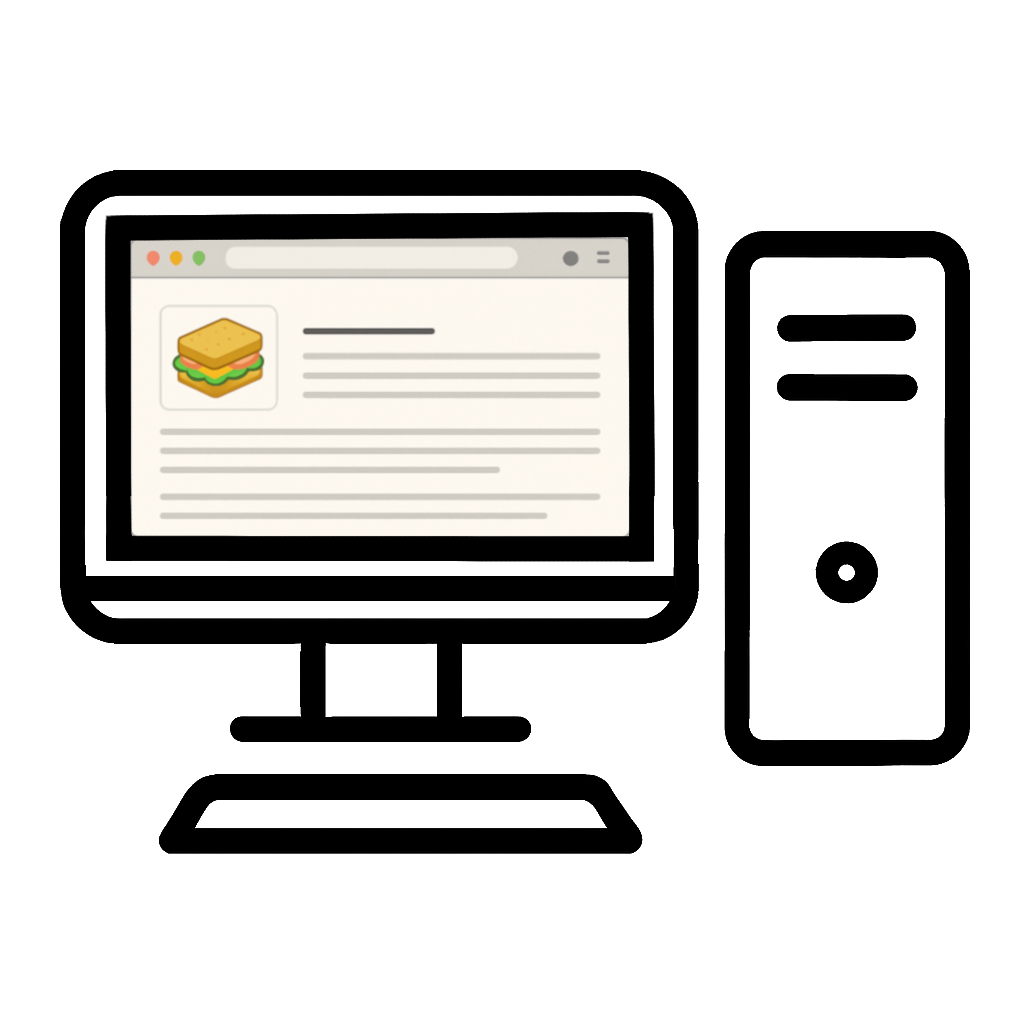
\includegraphics[width=1\textwidth]{./figures/computer_alpha_screen_2_website.png}
				\end{minipage}
			\end{adjustbox}
			\arrowx{\text{information}}
			\begin{adjustbox}{scale=1}
				\begin{minipage}{1\textwidth}
					
\includegraphics[width=0.8\textwidth]{./figures/evil_computer_scientist_alpha.png}
				\end{minipage}
			\end{adjustbox}
		\end{transformation}
		\vspace{-0.5cm}
		\begin{itemize}
			\item Information collected through web browser
			\item Privacy risk
		\end{itemize}
	\end{frame}

	\begin{frame}[fragile]{Browser-based device tracking}{Goldene image challenge}
		\begin{columns}
			\begin{column}{0.33\textwidth}
				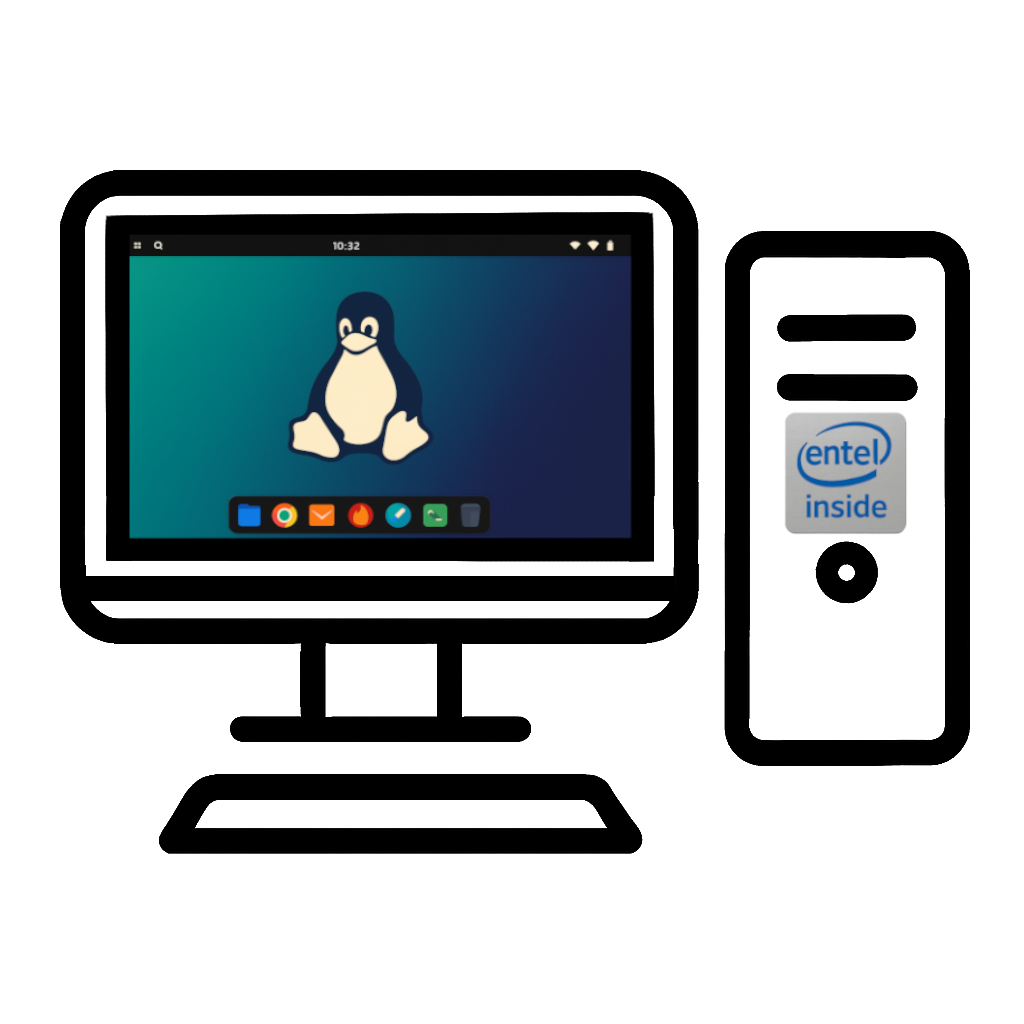
\includegraphics[width=1\textwidth]{./figures/computer_alpha_screen_2_golden.png}
			\end{column}
			\begin{column}{0.33\textwidth}
				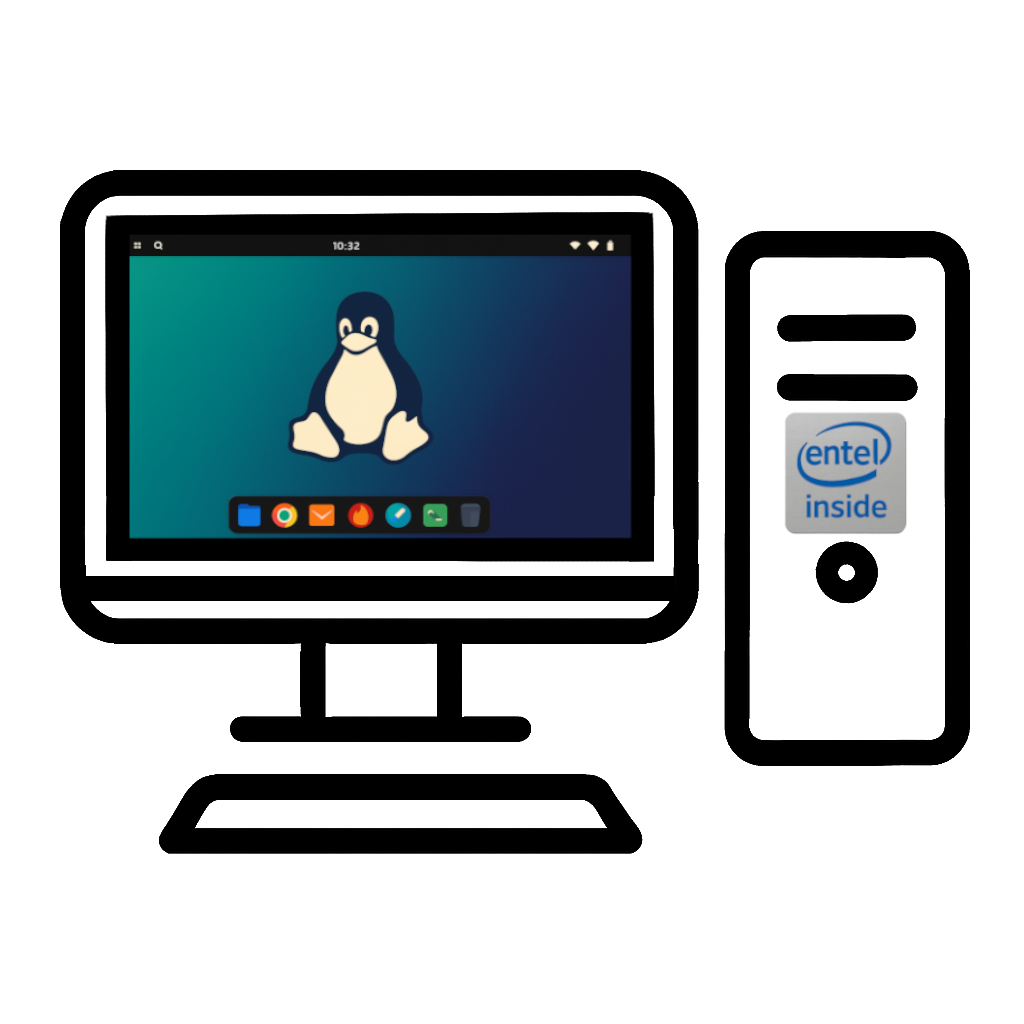
\includegraphics[width=1\textwidth]{./figures/computer_alpha_screen_2_golden.png}
			\end{column}
			\begin{column}{0.33\textwidth}
				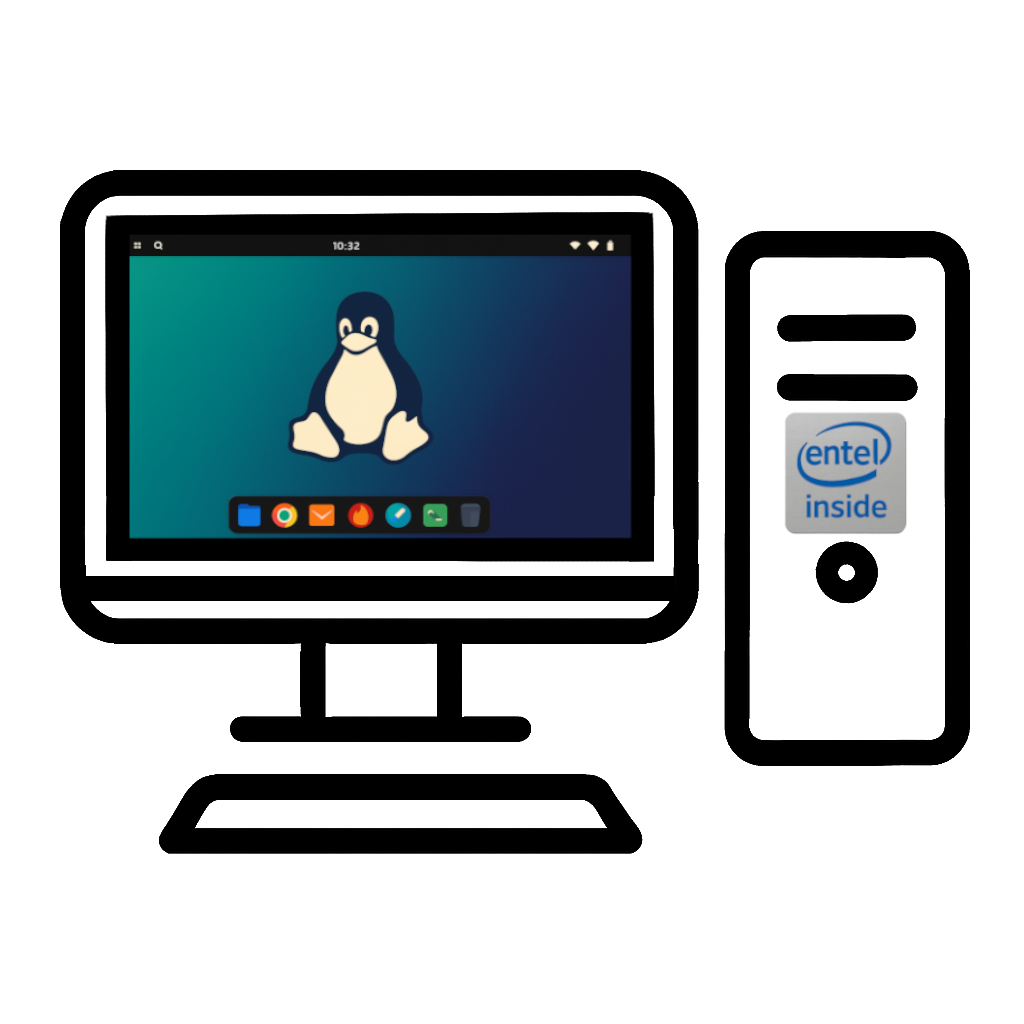
\includegraphics[width=1\textwidth]{./figures/computer_alpha_screen_2_golden.png}
			\end{column}
		\end{columns}
		\vspace{-0.5cm}
		\begin{itemize}
			\item \alert{Golden image challenge:} Distinguish identical devices with same hardware and software configuration \checkboxChecked \alert{$\Rightarrow$ device-specific key}
		\end{itemize}
	\end{frame}

	\begin{frame}[fragile]{Browser-based device tracking}{Types of techniques}
		\begin{itemize}
			\item \alert{Tagging techniques:} Insert an ID
			\begin{columns}
				\begin{column}{0.33\textwidth}
					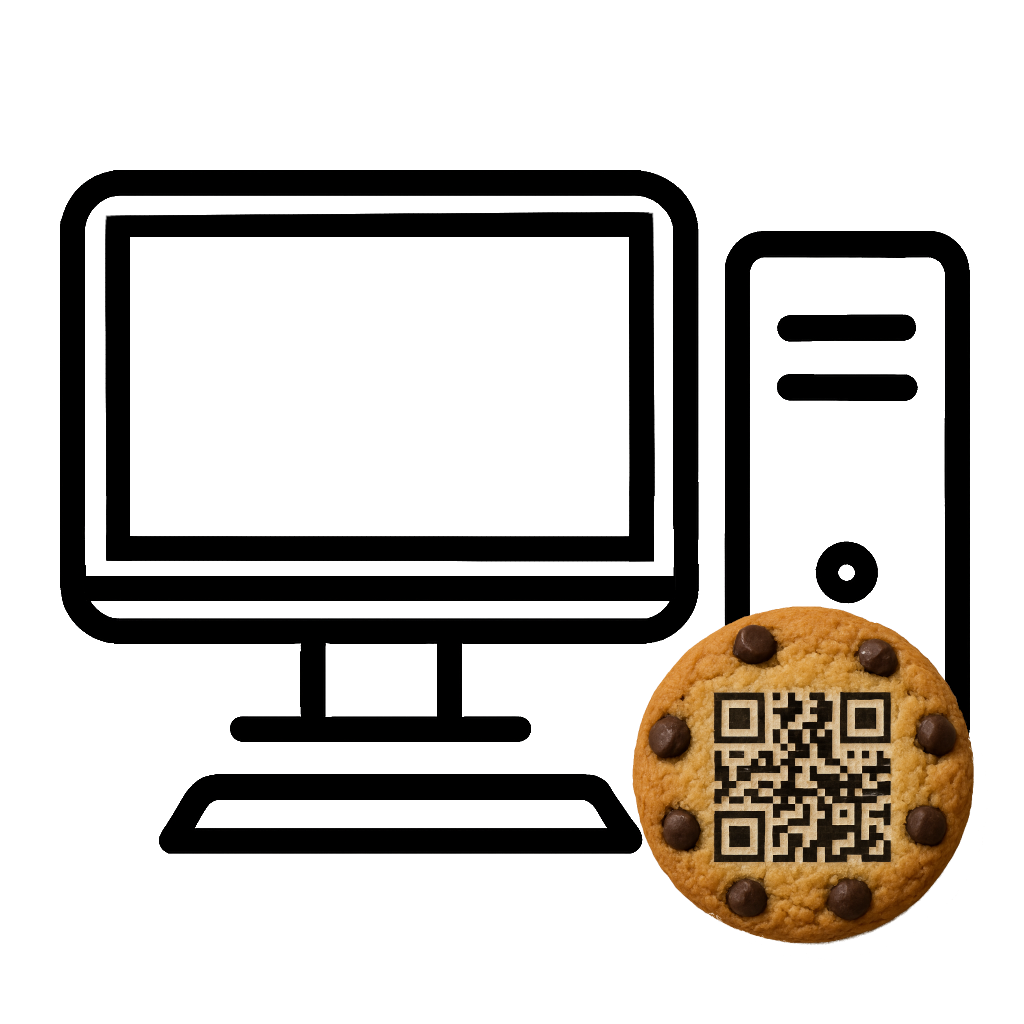
\includegraphics[width=0.5\textwidth, center]{./figures/computer_alpha_cookie_1.png}
				\end{column}
				\begin{column}{0.33\textwidth}
					
\includegraphics[width=0.5\textwidth, center]{./figures/computer_alpha_cookie_2.png}
				\end{column}
				\begin{column}{0.33\textwidth}
					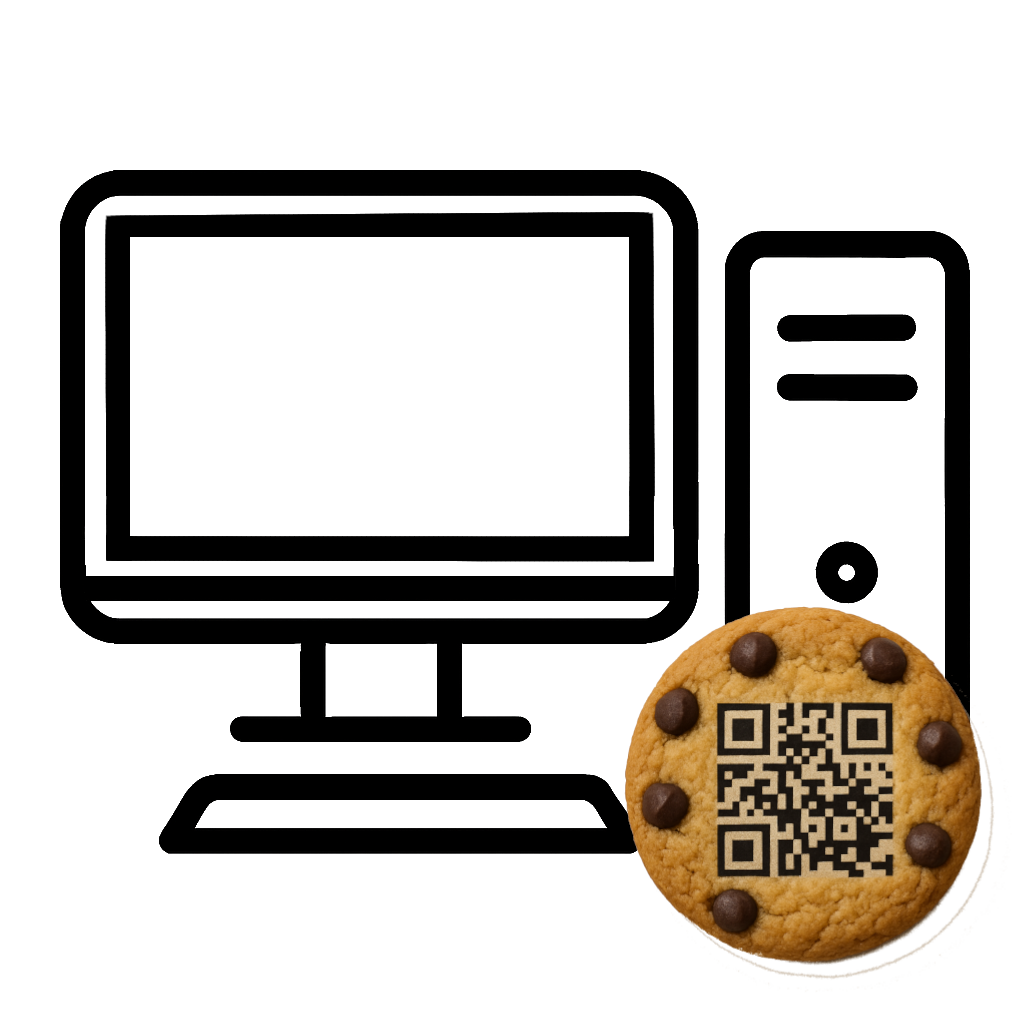
\includegraphics[width=0.5\textwidth, center]{./figures/computer_alpha_cookie_3.png}
				\end{column}
			\end{columns}
			\item \alert{Fingerprinting techniques:} Measure characteristics
			\begin{center}
				\begin{minipage}{0.7\textwidth}
					\begin{transformation}
						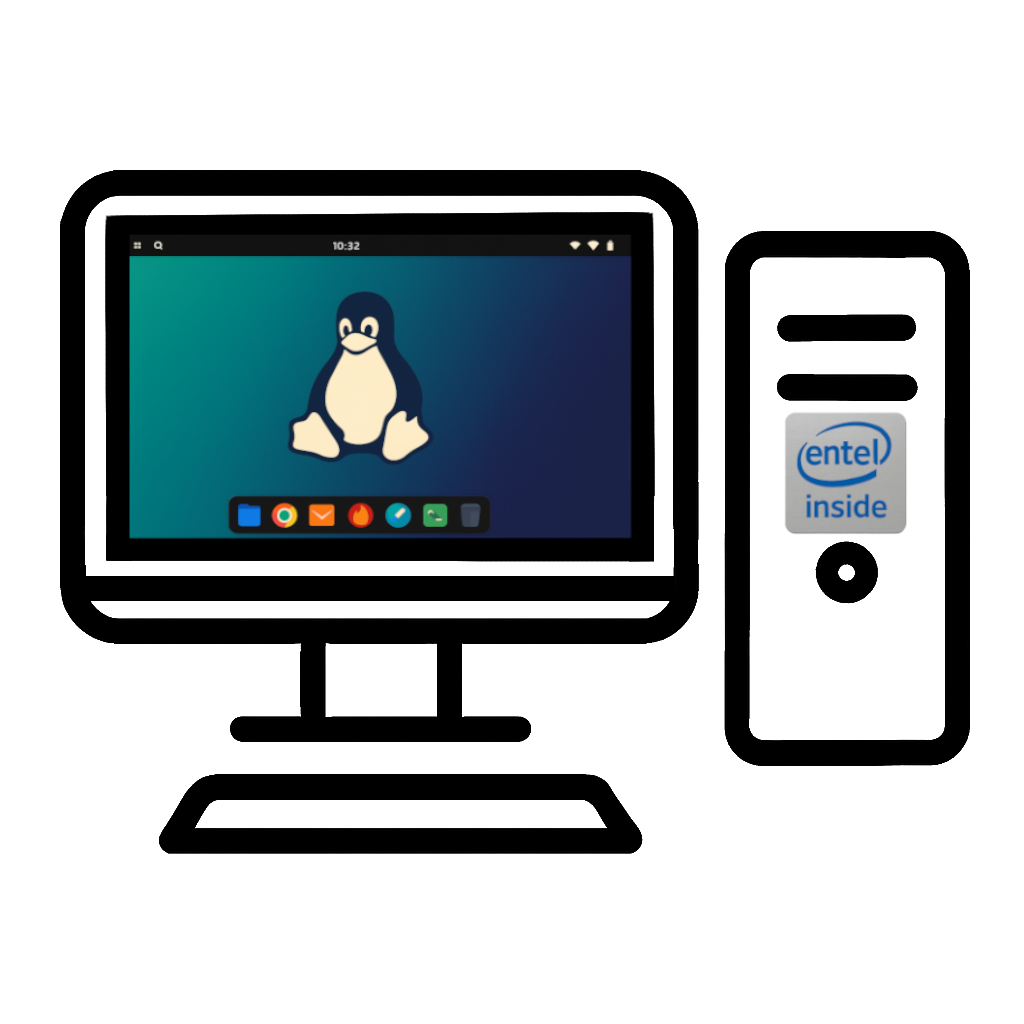
\includegraphics[width=0.7\textwidth]{./figures/computer_alpha_screen_2_golden.png}
						\arrowx{\text{generate fingerprint}}
						
\includegraphics[width=0.3\textwidth]{./figures/fingerprint.png}
					\end{transformation}
				\end{minipage}
			\end{center}
		\end{itemize}
		\begin{tikzpicture}[remember picture, overlay, shift={(current page.south west)}]
			\draw[thick, draw=PrimaryColor] (0.3cm,1.1cm) rectangle (13.2cm,4.2cm);
		\end{tikzpicture}
		% \grid
	\end{frame}

	\subsection{Source Port Selection}

	\begin{frame}[fragile]{Source Port Selection}{4-Tuple}
		\begin{itemize}
			\item \alert{4-tuple}: $(IP_{Src}, Port_{Src}, IP_{Dest}, Port_{Dest})$
			\begin{transformation}[0.2][0.6][0.2]
				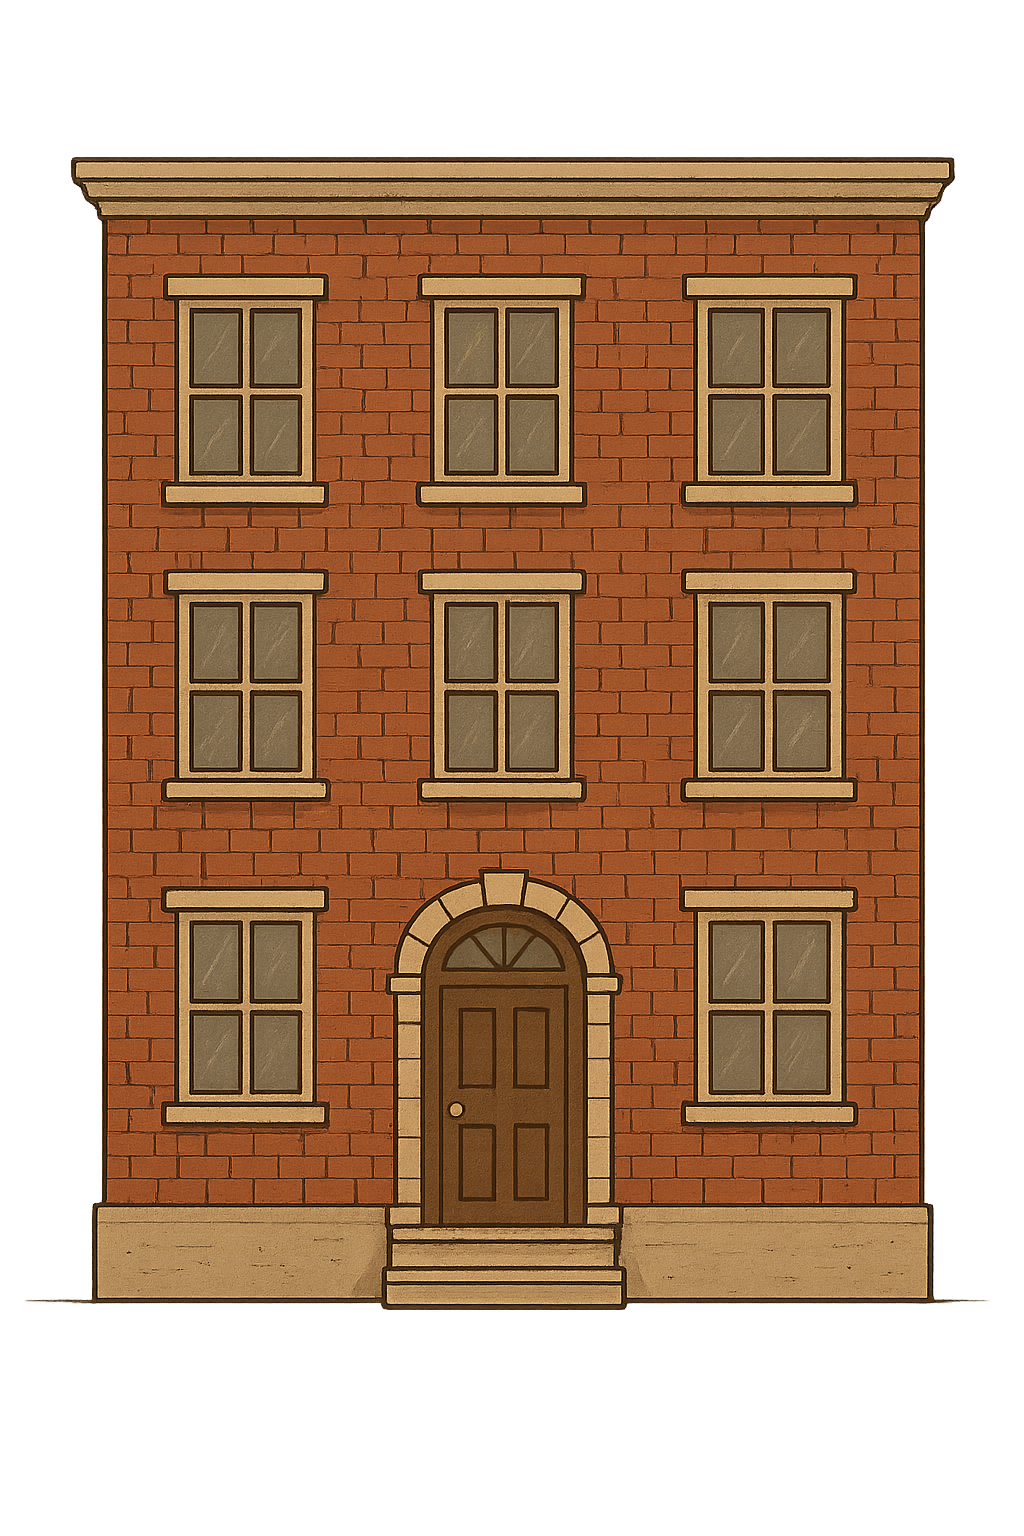
\includegraphics[width=\textwidth]{./figures/apartment1.png}
				\arrowxx{\text{(123 Maple St., Apt. 5B)}\hspace{1cm}\text{(456 Oak St., Apt. 9D)}}{\text{(192.0.2.123, 55'555)}\hspace{1cm}\text{(203.0.113.456, 49'999)}}
				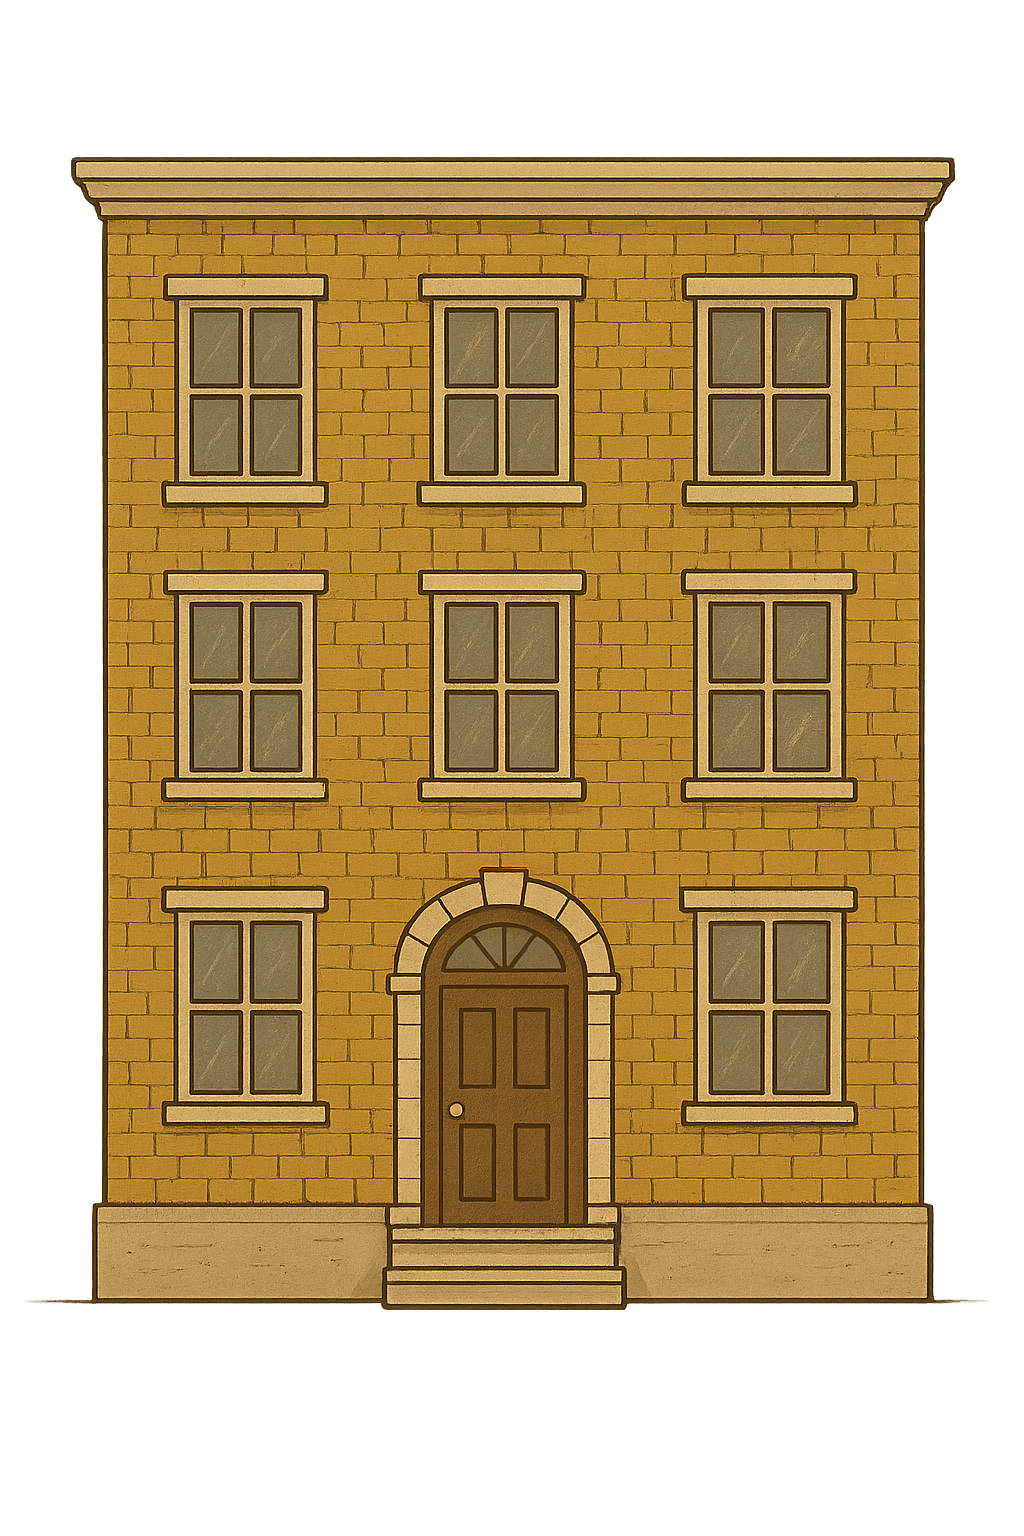
\includegraphics[width=\textwidth]{./figures/apartment2.png}
			\end{transformation}
			\vspace{-0.4cm}
			\begin{itemize}
				\scriptsize
				\item (192.0.2.123, 55'555, 203.0.113.10, 49'999)
				\item (123 Maple St., Apt. 5B, 456 Oak St., Apt. 9D)
			\end{itemize}
			\item Chooses TCP \alert{source port} $Port_{Src}$ for \alert{3-tuple}: $(IP_{Src}, IP_{Dest}, Port_{Dest})$
		\end{itemize}
	\end{frame}

	\begin{frame}[fragile]{Source Port Selection}{Goals}
		\begin{itemize}
			\item \alert{Functionality:} Reusing soure ports can cause failures
			\begin{itemize}
				\item[\alert{$\Rightarrow$}] Earlier connections might be active (\texttt{TIME\_WAIT} state)
			\end{itemize}
		\end{itemize}
		\begin{columns}
			\begin{column}[t]{0.33\textwidth}
				\vspace{2cm}

				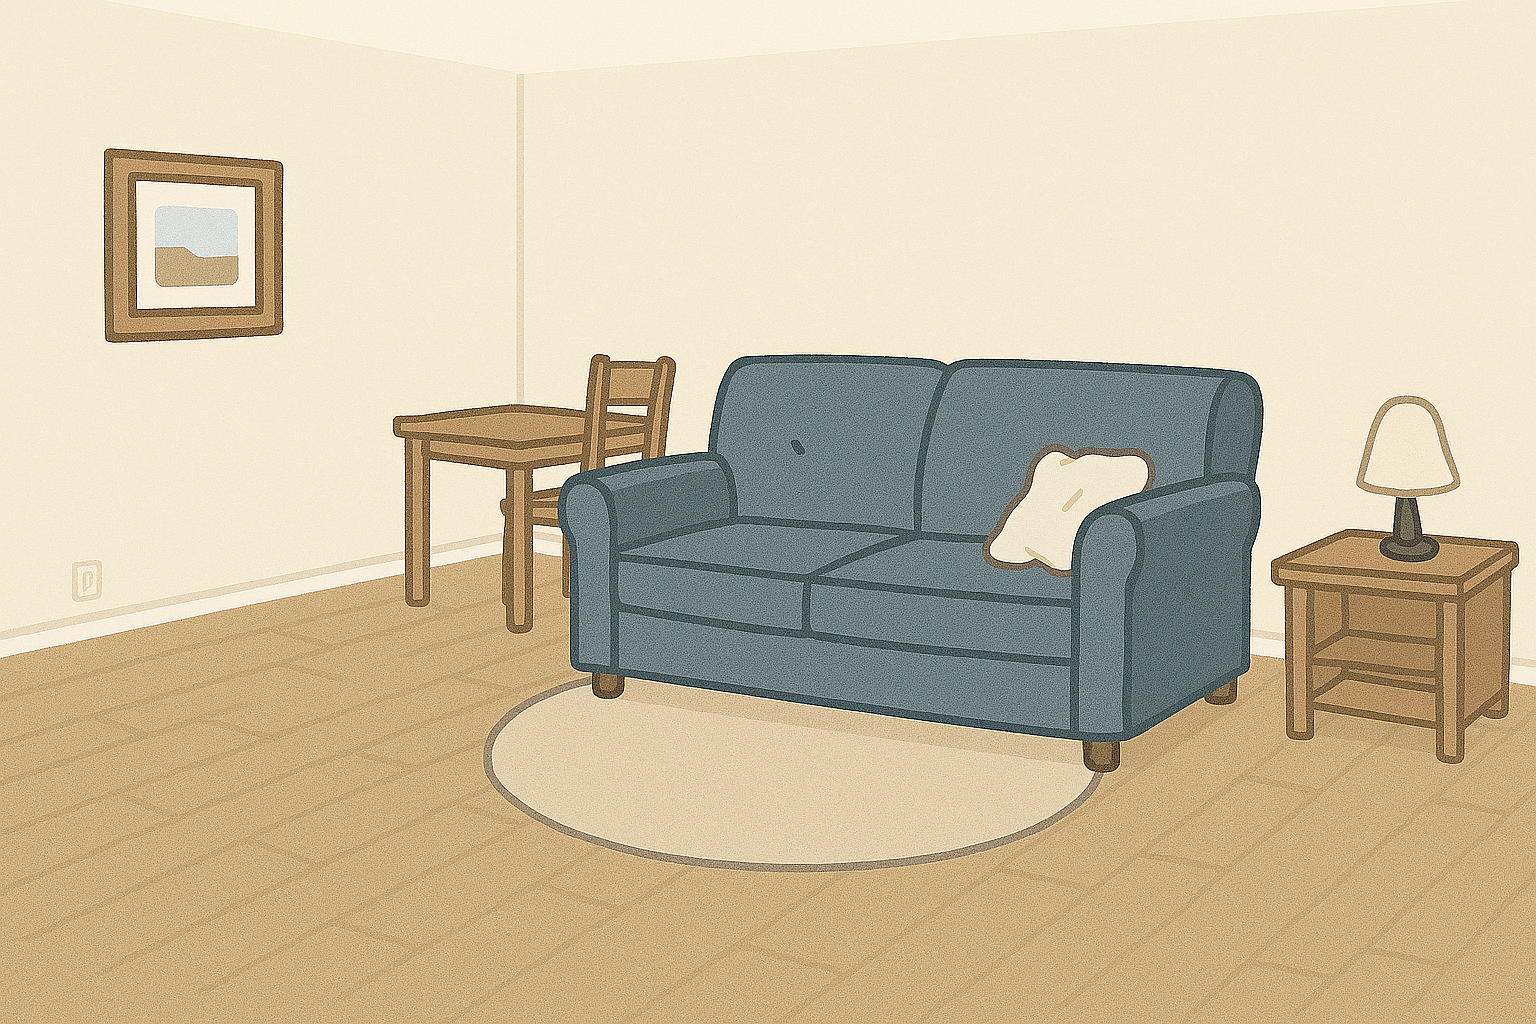
\includegraphics[width=0.8\textwidth, center]{./figures/room_cleaned.png}
			\end{column}
			\begin{column}[t]{0.33\textwidth}
				\vspace{0cm}

				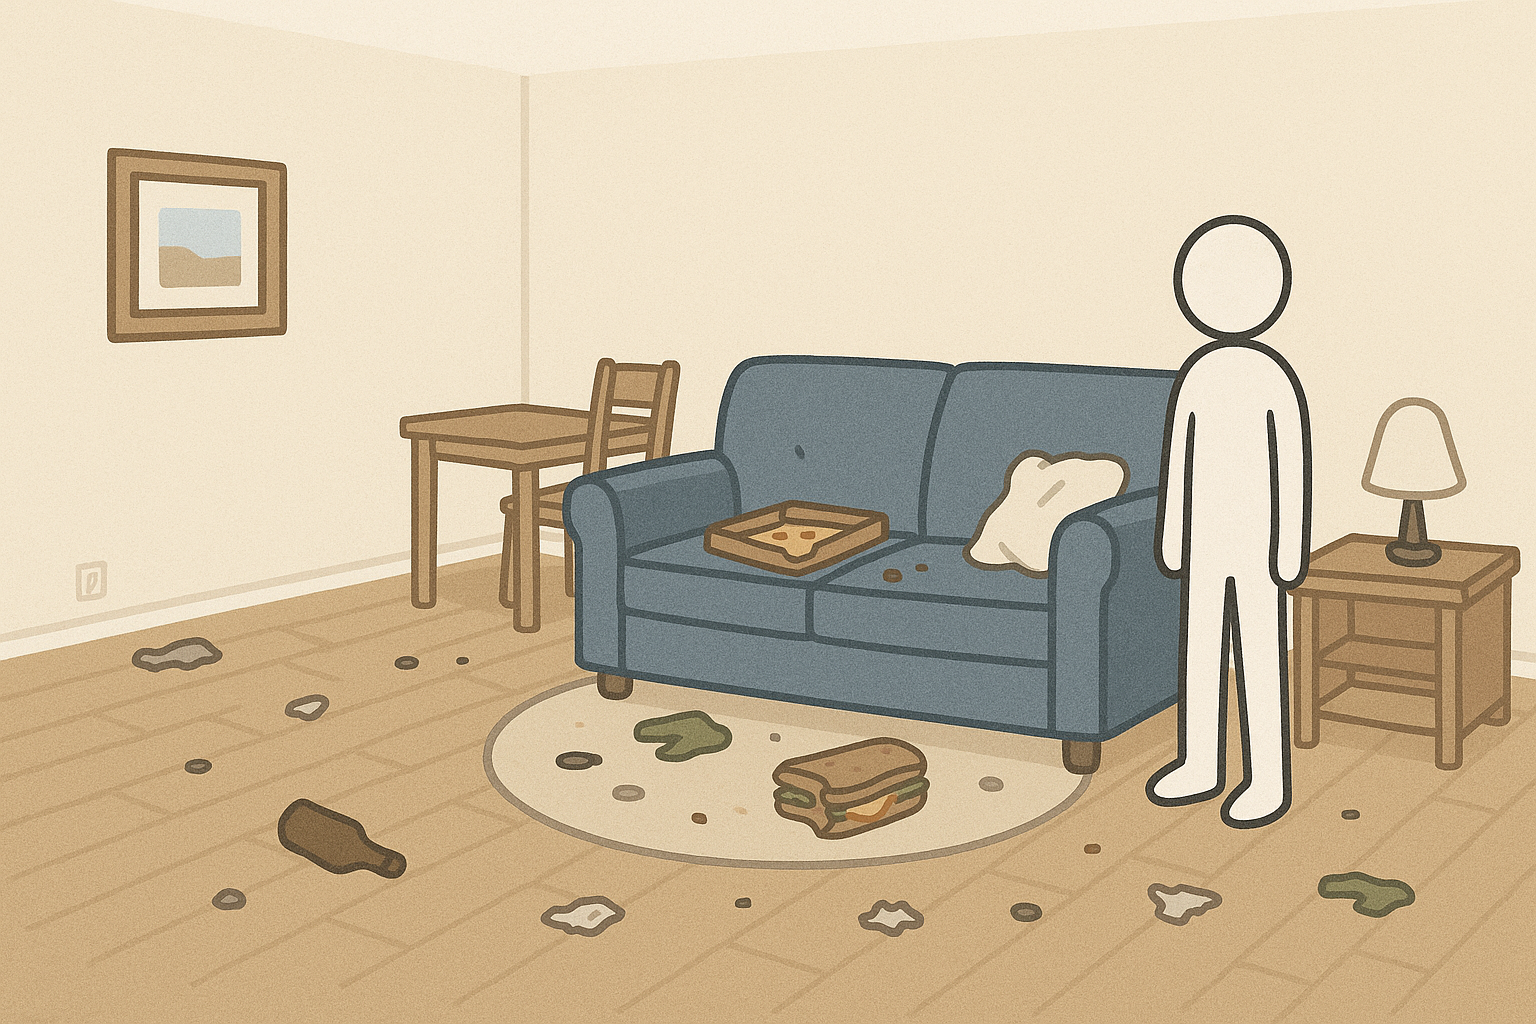
\includegraphics[width=0.8\textwidth, center]{./figures/room_not_cleaned.png}
			\end{column}
			\begin{column}[t]{0.33\textwidth}
				\vspace{0cm}

				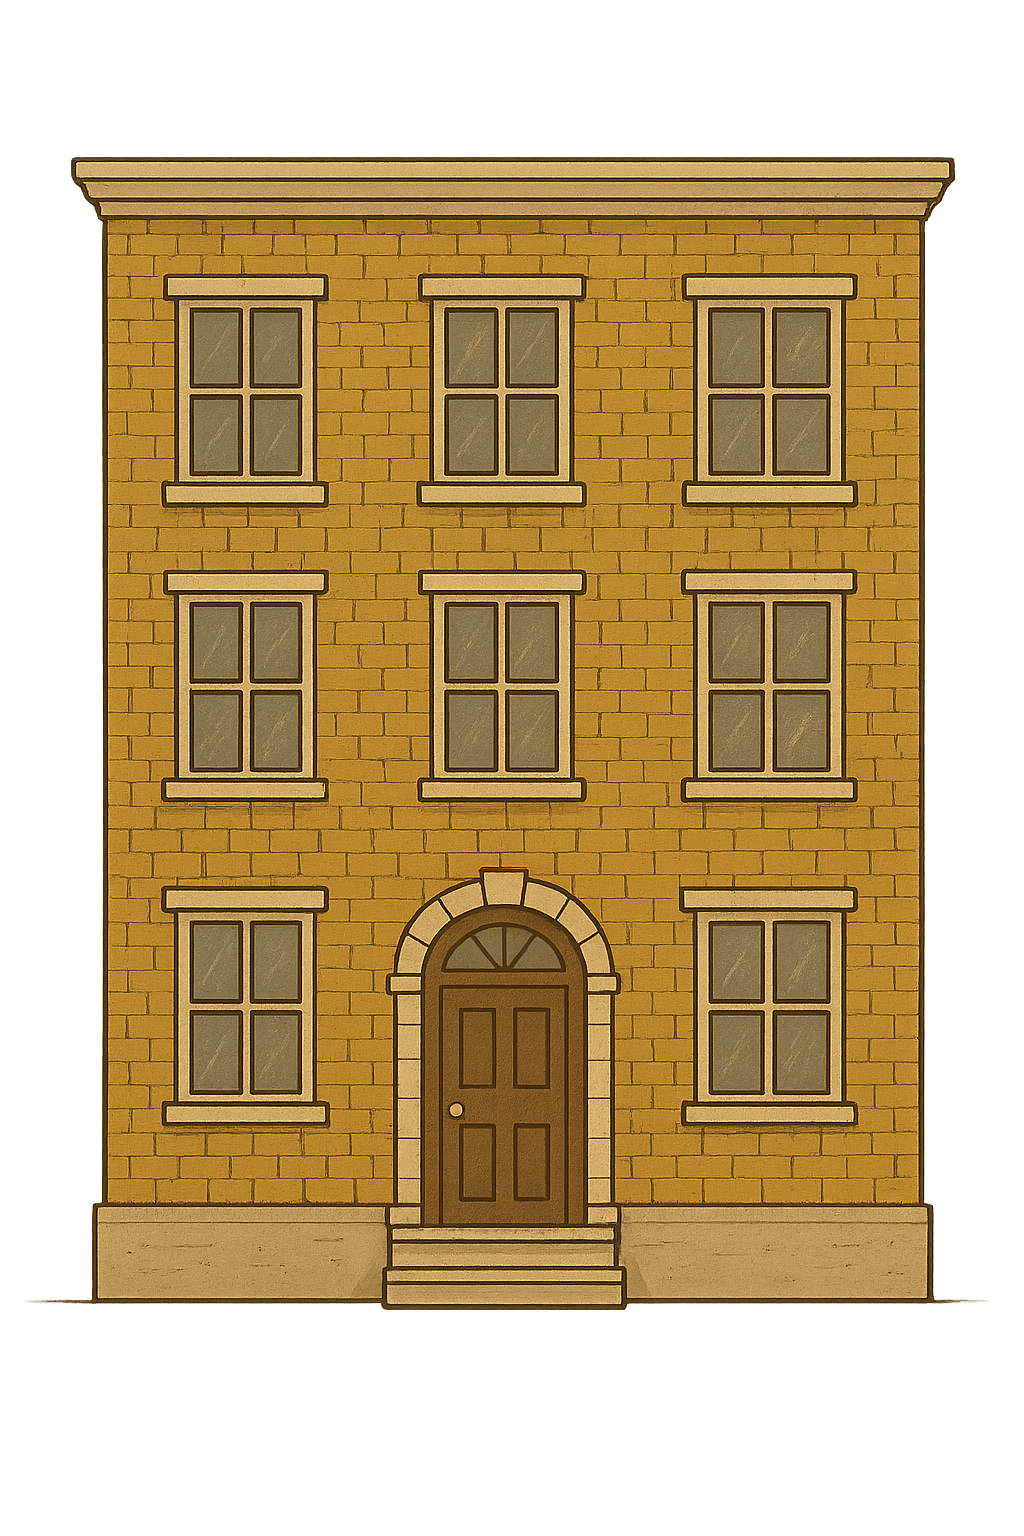
\includegraphics[width=0.8\textwidth, center]{./figures/apartment2.png}
			\end{column}
		\end{columns}
		\begin{tikzpicture}[remember picture, overlay, shift={(current page.south west)}]
			\draw[->, thick, draw=PrimaryColor] (4.35,2.3) -- (10.8,1.95);
			\draw[->, thick, draw=PrimaryColor] (9.1,4.3) -- (11.7,3.1);
		\end{tikzpicture}
		% \grid
	\end{frame}

	\begin{frame}[fragile]{Source Port Selection}{Goals}
		\begin{itemize}
			\item \alert{Security:}
			\begin{itemize}
				\item \alert{Off-path attacks} %like blind reset, data injection
				\item Determine \alert{Device activity (number TCP connections per time)} % if an attacker could, e.g., force a client to periodically establish a new TCP connection to an attacker-controlled machine (or through an attacker- observable path), the attacker could subtract consecutive source port values to obtain the number of outgoing TCP connections established globally by the target host within that time period 
			\end{itemize}
			\begin{transformation}[0.2][0.6][0.2]
				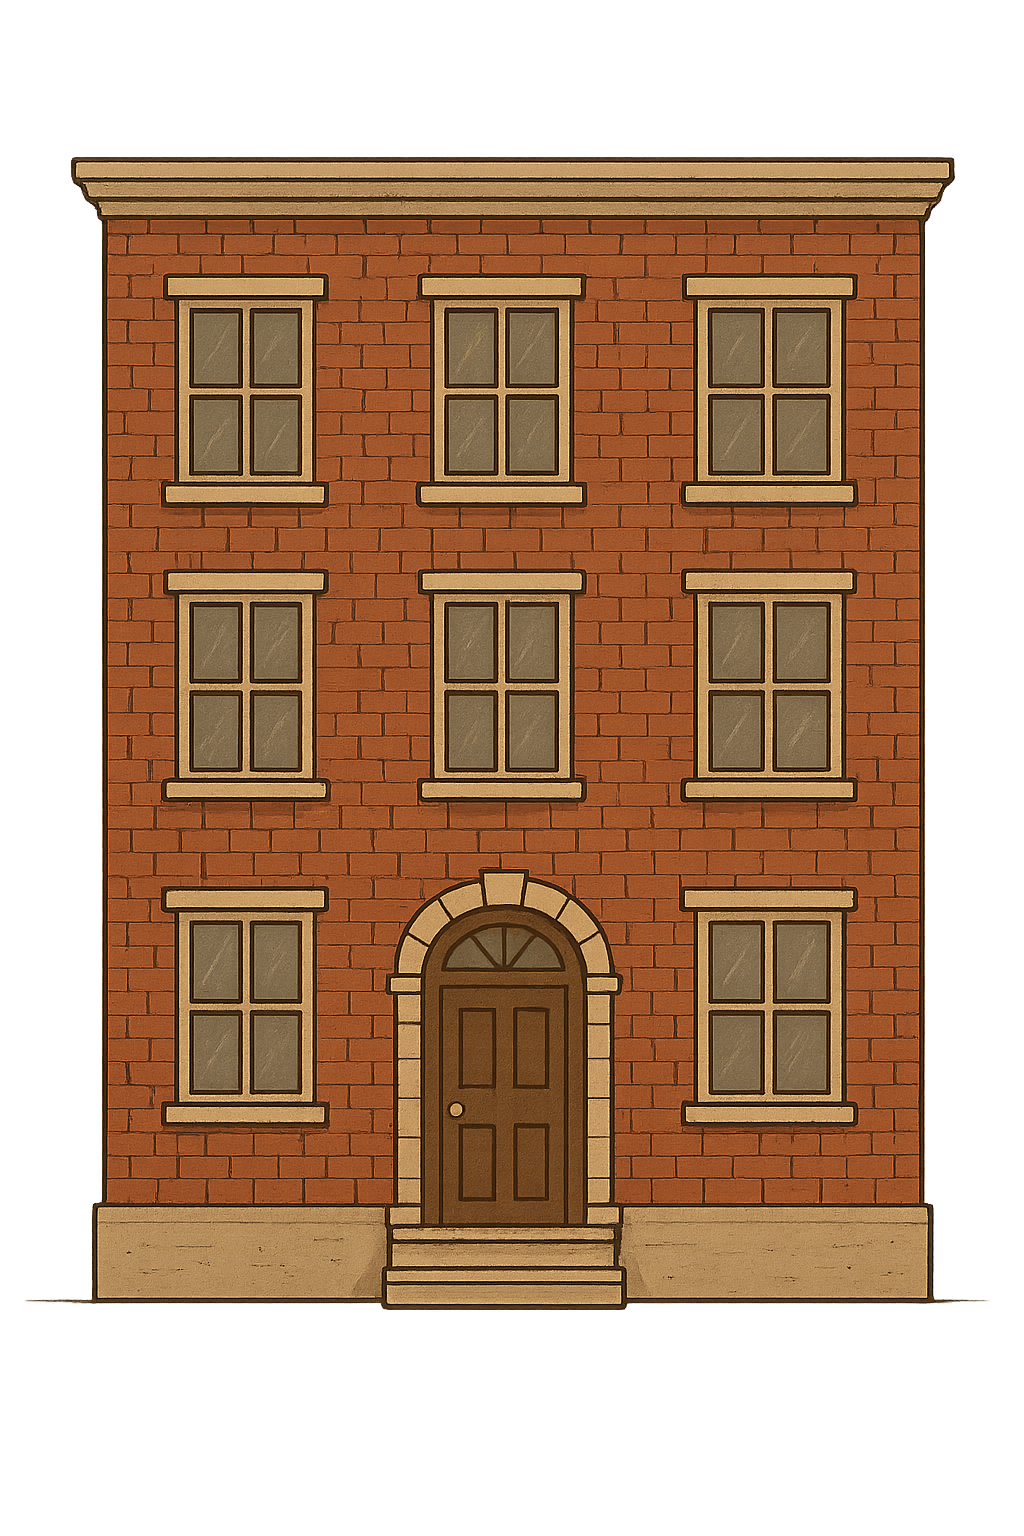
\includegraphics[width=\textwidth]{./figures/apartment1.png}
				\arrowxx{
\includegraphics[width=0.3\textwidth]{./figures/evil_computer_scientist_bicycle.png}}{\text{(123 Maple St., Apt. 5B)}\hspace{1cm}\text{(456 Oak St., Apt. 9D)}}
				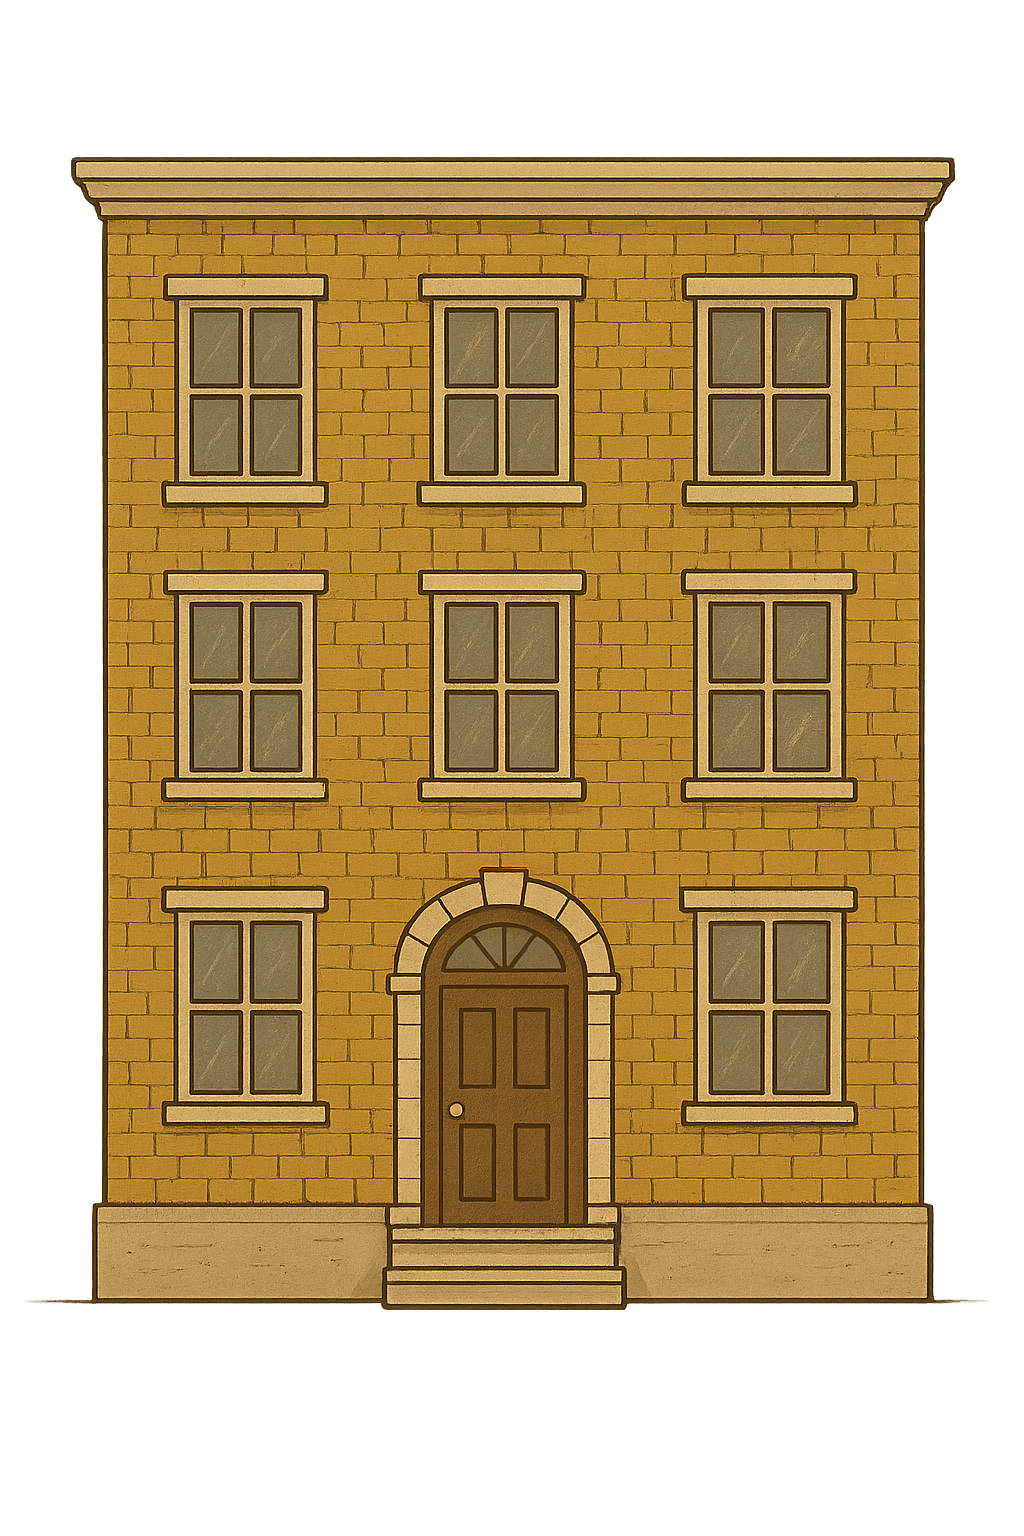
\includegraphics[width=\textwidth]{./figures/apartment2.png}
			\end{transformation}
		\end{itemize}
	\end{frame}

	\subsection{Double-Hash Port Selection Algorithm (DHPS)}

	\begin{frame}[fragile]{Double-Hash Port Selection Algorithm (DHPS)}{Algorithm Overview}
		\begin{itemize}
			\item TCP source ports divided into \alert{ranges}:

			\begin{adjustbox}{max width=0.9\textwidth}
				\begin{tblr}{
					colspec={|l|c|p{7cm}|},
					hlines,
					vlines,
					colsep=5pt,
					row{1} = {bg=PrimaryColor, fg=white, font=\bfseries},
					row{2} = {bg=PrimaryColorDimmed},
					row{3} = {bg=SecondaryColorDimmed},
					row{4} = {bg=PrimaryColorDimmed}
					}
					Port Range Type  & Typical Range & Usage                                                               \\
					Well-known ports & 0–1023        & Specific services, e.g. HTTP (80), HTTPS (443) etc.                 \\
					Registered ports & 1024–49151    & User applications or services, not ephemeral                        \\
					Ephemeral ports  & 49152–60999   & Dynamically allocated by OS for short-lived client-side connections \\
				\end{tblr}
			\end{adjustbox}
		\end{itemize}
		\begin{tikzpicture}[remember picture, overlay, shift={(current page.south west)}]
			\draw[thick, draw=PrimaryColor] (0.9cm,2.23cm) rectangle (13.2cm,3.22cm);
			\draw[->, thick, draw=PrimaryColor] (14.3,2.75) -- (13.3,2.75);
		\end{tikzpicture}
		% \grid
	\end{frame}

	\begin{frame}[fragile]{Double-Hash Port Selection Algorithm (DHPS)}{Algorithm Overview}
		\begin{itemize}
			\item \alert{Complete 3-tuple to 4-tuple} with cryptographic keyed-hash functions:
			\begin{itemize}
				\scriptsize
				\item \( F_{K_1}: \text{3-Tuples} \xrightarrow{K_1} \{0, \ldots, 2^{32}\}\)
				\item \( G_{K_2}: \text{3-Tuples} \xrightarrow{K_2} \{0, \ldots, T\}\) where $T$ is length of \alert{perturbation table}
			\end{itemize}
		\end{itemize}
		\begin{columns}
			\begin{column}{0.5\textwidth}
				\begin{itemize}
					\item Incrementation of port numbers separated into \alert{$T$ different spaces}
					\begin{itemize}
						\item[\alert{$\Rightarrow$}] Port-reuse frequency lower\cite{larsenRecommendationsTransportProtocolPort2011} % (probabilistically) 
						\item[\alert{$\Rightarrow$}] Harder to analyse device activity % if an attacker could, e.g., force a client to periodically establish a new TCP connection to an attacker-controlled machine (or through an attacker- observable path), the attacker could subtract consecutive source port values to obtain the number of outgoing TCP connections established globally by the target host within that time period
					\end{itemize}
				\end{itemize}
			\end{column}
			\begin{column}{0.5\textwidth}
				\begin{center}
					\begin{adjustbox}{max width=\textwidth}
						\tikzfig{perturbation_table} % ./figures/perturbation_table.tikz
					\end{adjustbox}
				\end{center}
			\end{column}
		\end{columns}
		% Further increasing the TABLE_LENGTH will increase the unpredictability of the resulting port number, and possibly further decrease the collision rate
	\end{frame}

	\begin{frame}[fragile]{Double-Hash Port Selection Algorithm (DHPS)}{Pseudocode}
		\begin{adjustbox}{scale=0.8}
			\begin{minipage}{0.8\textwidth}
				%!Tex Root = ../main.tex

\begin{algorithm}{\pr{DHPS Source Port Selection}}{\thetcbcounter}\label{alg:dhps_port_selection}
	\begin{pseudo}[indent-mark,kw,hl-warn=false]
		procedure \cn{SelectEphemeralPort} \\+
		\tt{num\_ephemeral} $\leftarrow \tt{max\_ephemeral} - \tt{min\_ephemeral}+\tn{1}$ \\
    \tt{offset} $\leftarrow$ $\cn{F}_{K_1}$($\tt{IP}_{SRC}$,$\tt{IP}_{DST}$,$\tt{PORT}_{DST}$) \\
    \tt{index} $\leftarrow$ $\cn{G}_{K_2}$($\tt{IP}_{SRC}$,$\tt{IP}_{DST}$,$\tt{PORT}_{DST}$) \\
		\tt{count} $\leftarrow$ \tt{num\_ephemeral} \\
		repeat \\+
		$\tt{port} $\leftarrow$ \tt{min\_ephemeral}$+\\+
		$((\tt{offset}+\tt{table[index]})$ $mod$ $\tt{num\_ephemeral})$ \\-
		$\tt{table[index]} $\leftarrow$ \tt{table[index]} +\tn{1}$ \\
		if \cn{CheckSuitablePort}(\tt{port}) then \\+
		return \tt{port} \\-
		$\tt{count} $\leftarrow$ \tt{count} - \tn{1}$ \\-
		until \tt{count} = \tn{0} \\
		return \tt{Error}\\
	\end{pseudo}
\end{algorithm}

			\end{minipage}
		\end{adjustbox}
		\begin{tikzpicture}[remember picture, overlay, shift={(current page.south west)}] % 1
			\node[anchor=north west]  at (9.3cm, 5.8cm) {%
				\includegraphics[scale=0.7]{./figures/external/dhps_source_port_calculation_2.pdf}
			};
		\end{tikzpicture}
		\begin{tikzpicture}[remember picture, overlay, shift={(current page.south west)}]
			\node[anchor=north west] at (9cm, 7.1cm) {%
				\begin{minipage}{\textwidth}
					\begin{itemize}
		         \item \alert{Source port calculation:}
						\begin{itemize}
		           \scriptsize
							\item $offset=50'000$
							\item $index=255$
						\end{itemize}
					\end{itemize}
				\end{minipage}
			};
		\end{tikzpicture}
		% \begin{tikzpicture}[remember picture, overlay, shift={(current page.south west)}] % 2
		% 	\node[anchor=north west]  at (9.4cm, 5.8cm) {%
		% 		\includegraphics[scale=0.7]{./figures/external/dhps_source_port_calculation_increment.pdf}
		% 	};
		% \end{tikzpicture}
		% \begin{tikzpicture}[remember picture, overlay, shift={(current page.south west)}]
		% 	\node[anchor=north west] at (9.3cm, 7.1cm) {%
		% 		\begin{minipage}{\textwidth}
		% 			\begin{itemize}
		% 				\item \alert{Source port calculation:}
		% 				\begin{itemize}
		% 					\scriptsize
		% 					\item $offset=50'000$
		% 					\item $index=255$
		% 				\end{itemize}
		% 			\end{itemize}
		% 		\end{minipage}
		% 	};
		% \end{tikzpicture}
		\begin{tikzpicture}[remember picture, overlay, shift={(current page.south west)}]
			% source port calculation % 1
			\draw[thick, draw=PrimaryColor] (1.5cm,5.0cm) rectangle (6.75cm,5.45cm);
			\draw[thick, draw=PrimaryColor] (1.5cm,4.6cm) rectangle (6.65cm,5.0cm);
			\draw[thick, draw=PrimaryColor] (2.1cm,3.1cm) rectangle (9.15cm,3.9cm);
			% increase of table entry % 2
			% \draw[thick, draw=PrimaryColor] (2.1cm,2.75cm) rectangle (6.85cm,3.1cm);
			% \draw[thick, draw=PrimaryColor] (2.1cm,1.95cm) rectangle (7.25cm,2.75cm);
			% loop termiation
			% \draw[thick, draw=PrimaryColor] (1.5cm,4.25cm) rectangle (4.8cm,4.6cm);
			% \draw[thick, draw=PrimaryColor] (2.1cm,1.6cm) rectangle (4.55cm,1.95cm);
			% \draw[thick, draw=PrimaryColor] (1.5cm,1.2cm) rectangle (3.75cm,1.6cm);
			% terminate with error
			% \draw[thick, draw=PrimaryColor] (1.5cm,0.75cm) rectangle (3.35cm,1.2cm);
		\end{tikzpicture}
		% \grid
	\end{frame}

	\begin{frame}[fragile]{Double-Hash Port Selection Algorithm (DHPS)}{Pseudocode}
		\begin{adjustbox}{scale=0.8}
			\begin{minipage}{0.8\textwidth}
				%!Tex Root = ../main.tex

\begin{algorithm}{\pr{DHPS Source Port Selection}}{\thetcbcounter}\label{alg:dhps_port_selection}
	\begin{pseudo}[indent-mark,kw,hl-warn=false]
		procedure \cn{SelectEphemeralPort} \\+
		\tt{num\_ephemeral} $\leftarrow \tt{max\_ephemeral} - \tt{min\_ephemeral}+\tn{1}$ \\
    \tt{offset} $\leftarrow$ $\cn{F}_{K_1}$($\tt{IP}_{SRC}$,$\tt{IP}_{DST}$,$\tt{PORT}_{DST}$) \\
    \tt{index} $\leftarrow$ $\cn{G}_{K_2}$($\tt{IP}_{SRC}$,$\tt{IP}_{DST}$,$\tt{PORT}_{DST}$) \\
		\tt{count} $\leftarrow$ \tt{num\_ephemeral} \\
		repeat \\+
		$\tt{port} $\leftarrow$ \tt{min\_ephemeral}$+\\+
		$((\tt{offset}+\tt{table[index]})$ $mod$ $\tt{num\_ephemeral})$ \\-
		$\tt{table[index]} $\leftarrow$ \tt{table[index]} +\tn{1}$ \\
		if \cn{CheckSuitablePort}(\tt{port}) then \\+
		return \tt{port} \\-
		$\tt{count} $\leftarrow$ \tt{count} - \tn{1}$ \\-
		until \tt{count} = \tn{0} \\
		return \tt{Error}\\
	\end{pseudo}
\end{algorithm}

			\end{minipage}
		\end{adjustbox}
		% \begin{tikzpicture}[remember picture, overlay, shift={(current page.south west)}] % 1
		% 	\node[anchor=north west]  at (9.3cm, 5.8cm) {%
		% 		\includegraphics[scale=0.7]{./figures/external/dhps_source_port_calculation_2.pdf}
		% 	};
		% \end{tikzpicture}
		% \begin{tikzpicture}[remember picture, overlay, shift={(current page.south west)}]
		% 	\node[anchor=north west] at (9cm, 7.1cm) {%
		% 		\begin{minipage}{\textwidth}
		% 			\begin{itemize}
		%          \item \alert{Source port calculation:}
		% 				\begin{itemize}
		%            \scriptsize
		% 					\item $offset=50'000$
		% 					\item $index=255$
		% 				\end{itemize}
		% 			\end{itemize}
		% 		\end{minipage}
		% 	};
		% \end{tikzpicture}
		\begin{tikzpicture}[remember picture, overlay, shift={(current page.south west)}] % 2
			\node[anchor=north west]  at (9.4cm, 5.8cm) {%
				\includegraphics[scale=0.7]{./figures/external/dhps_source_port_calculation_increment.pdf}
			};
		\end{tikzpicture}
		\begin{tikzpicture}[remember picture, overlay, shift={(current page.south west)}]
			\node[anchor=north west] at (9.3cm, 7.1cm) {%
				\begin{minipage}{\textwidth}
					\begin{itemize}
						\item \alert{Source port calculation:}
						\begin{itemize}
							\scriptsize
							\item $offset=50'000$
							\item $index=255$
						\end{itemize}
					\end{itemize}
				\end{minipage}
			};
		\end{tikzpicture}
		\begin{tikzpicture}[remember picture, overlay, shift={(current page.south west)}]
			% source port calculation % 1
			% \draw[thick, draw=PrimaryColor] (1.5cm,5.0cm) rectangle (6.75cm,5.45cm);
			% \draw[thick, draw=PrimaryColor] (1.5cm,4.6cm) rectangle (6.65cm,5.0cm);
			% \draw[thick, draw=PrimaryColor] (2.1cm,3.1cm) rectangle (9.15cm,3.9cm);
			% increase of table entry % 2
			\draw[thick, draw=PrimaryColor] (2.1cm,2.75cm) rectangle (6.85cm,3.1cm);
			\draw[thick, draw=PrimaryColor] (2.1cm,1.95cm) rectangle (7.25cm,2.75cm);
			% loop termiation
			% \draw[thick, draw=PrimaryColor] (1.5cm,4.25cm) rectangle (4.8cm,4.6cm);
			% \draw[thick, draw=PrimaryColor] (2.1cm,1.6cm) rectangle (4.55cm,1.95cm);
			% \draw[thick, draw=PrimaryColor] (1.5cm,1.2cm) rectangle (3.75cm,1.6cm);
			% terminate with error
			% \draw[thick, draw=PrimaryColor] (1.5cm,0.75cm) rectangle (3.35cm,1.2cm);
		\end{tikzpicture}
		% \grid
	\end{frame}

	\begin{frame}[fragile]{Double-Hash Port Selection Algorithm (DHPS)}{Pseudocode}
		\begin{adjustbox}{scale=0.8}
			\begin{minipage}{0.8\textwidth}
				%!Tex Root = ../main.tex

\begin{algorithm}{\pr{DHPS Source Port Selection}}{\thetcbcounter}\label{alg:dhps_port_selection}
	\begin{pseudo}[indent-mark,kw,hl-warn=false]
		procedure \cn{SelectEphemeralPort} \\+
		\tt{num\_ephemeral} $\leftarrow \tt{max\_ephemeral} - \tt{min\_ephemeral}+\tn{1}$ \\
    \tt{offset} $\leftarrow$ $\cn{F}_{K_1}$($\tt{IP}_{SRC}$,$\tt{IP}_{DST}$,$\tt{PORT}_{DST}$) \\
    \tt{index} $\leftarrow$ $\cn{G}_{K_2}$($\tt{IP}_{SRC}$,$\tt{IP}_{DST}$,$\tt{PORT}_{DST}$) \\
		\tt{count} $\leftarrow$ \tt{num\_ephemeral} \\
		repeat \\+
		$\tt{port} $\leftarrow$ \tt{min\_ephemeral}$+\\+
		$((\tt{offset}+\tt{table[index]})$ $mod$ $\tt{num\_ephemeral})$ \\-
		$\tt{table[index]} $\leftarrow$ \tt{table[index]} +\tn{1}$ \\
		if \cn{CheckSuitablePort}(\tt{port}) then \\+
		return \tt{port} \\-
		$\tt{count} $\leftarrow$ \tt{count} - \tn{1}$ \\-
		until \tt{count} = \tn{0} \\
		return \tt{Error}\\
	\end{pseudo}
\end{algorithm}

			\end{minipage}
		\end{adjustbox}
		% \begin{tikzpicture}[remember picture, overlay, shift={(current page.south west)}] % 1
		% 	\node[anchor=north west]  at (9.3cm, 5.8cm) {%
		% 		\includegraphics[scale=0.7]{./figures/external/dhps_source_port_calculation_2.pdf}
		% 	};
		% \end{tikzpicture}
		% \begin{tikzpicture}[remember picture, overlay, shift={(current page.south west)}]
		% 	\node[anchor=north west] at (9cm, 7.1cm) {%
		% 		\begin{minipage}{\textwidth}
		% 			\begin{itemize}
		%          \item \alert{Source port calculation:}
		% 				\begin{itemize}
		%            \scriptsize
		% 					\item $offset=50'000$
		% 					\item $index=255$
		% 				\end{itemize}
		% 			\end{itemize}
		% 		\end{minipage}
		% 	};
		% \end{tikzpicture}
		\begin{tikzpicture}[remember picture, overlay, shift={(current page.south west)}] % 2
			\node[anchor=north west]  at (9.4cm, 5.8cm) {%
				\includegraphics[scale=0.7]{./figures/external/dhps_source_port_calculation_increment.pdf}
			};
		\end{tikzpicture}
		\begin{tikzpicture}[remember picture, overlay, shift={(current page.south west)}]
			\node[anchor=north west] at (9.3cm, 7.1cm) {%
				\begin{minipage}{\textwidth}
					\begin{itemize}
						\item \alert{Source port calculation:}
						\begin{itemize}
							\scriptsize
							\item $offset=50'000$
							\item $index=255$
						\end{itemize}
					\end{itemize}
				\end{minipage}
			};
		\end{tikzpicture}
		\begin{tikzpicture}[remember picture, overlay, shift={(current page.south west)}]
			% source port calculation % 1
			% \draw[thick, draw=PrimaryColor] (1.5cm,5.0cm) rectangle (6.75cm,5.45cm);
			% \draw[thick, draw=PrimaryColor] (1.5cm,4.6cm) rectangle (6.65cm,5.0cm);
			% \draw[thick, draw=PrimaryColor] (2.1cm,3.1cm) rectangle (9.15cm,3.9cm);
			% increase of table entry % 2
			% \draw[thick, draw=PrimaryColor] (2.1cm,2.75cm) rectangle (6.85cm,3.1cm);
			% \draw[thick, draw=PrimaryColor] (2.1cm,1.95cm) rectangle (7.25cm,2.75cm);
			% loop termiation
			\draw[thick, draw=PrimaryColor] (1.5cm,4.25cm) rectangle (4.8cm,4.6cm);
			\draw[thick, draw=PrimaryColor] (2.1cm,1.6cm) rectangle (4.55cm,1.95cm);
			\draw[thick, draw=PrimaryColor] (1.5cm,1.2cm) rectangle (3.75cm,1.6cm);
			% terminate with error
			% \draw[thick, draw=PrimaryColor] (1.5cm,0.75cm) rectangle (3.35cm,1.2cm);
		\end{tikzpicture}
		% \grid
	\end{frame}

	\begin{frame}[fragile]{Double-Hash Port Selection Algorithm (DHPS)}{Pseudocode}
		\begin{adjustbox}{scale=0.8}
			\begin{minipage}{0.8\textwidth}
				%!Tex Root = ../main.tex

\begin{algorithm}{\pr{DHPS Source Port Selection}}{\thetcbcounter}\label{alg:dhps_port_selection}
	\begin{pseudo}[indent-mark,kw,hl-warn=false]
		procedure \cn{SelectEphemeralPort} \\+
		\tt{num\_ephemeral} $\leftarrow \tt{max\_ephemeral} - \tt{min\_ephemeral}+\tn{1}$ \\
    \tt{offset} $\leftarrow$ $\cn{F}_{K_1}$($\tt{IP}_{SRC}$,$\tt{IP}_{DST}$,$\tt{PORT}_{DST}$) \\
    \tt{index} $\leftarrow$ $\cn{G}_{K_2}$($\tt{IP}_{SRC}$,$\tt{IP}_{DST}$,$\tt{PORT}_{DST}$) \\
		\tt{count} $\leftarrow$ \tt{num\_ephemeral} \\
		repeat \\+
		$\tt{port} $\leftarrow$ \tt{min\_ephemeral}$+\\+
		$((\tt{offset}+\tt{table[index]})$ $mod$ $\tt{num\_ephemeral})$ \\-
		$\tt{table[index]} $\leftarrow$ \tt{table[index]} +\tn{1}$ \\
		if \cn{CheckSuitablePort}(\tt{port}) then \\+
		return \tt{port} \\-
		$\tt{count} $\leftarrow$ \tt{count} - \tn{1}$ \\-
		until \tt{count} = \tn{0} \\
		return \tt{Error}\\
	\end{pseudo}
\end{algorithm}

			\end{minipage}
		\end{adjustbox}
		% \begin{tikzpicture}[remember picture, overlay, shift={(current page.south west)}] % 1
		% 	\node[anchor=north west]  at (9.3cm, 5.8cm) {%
		% 		\includegraphics[scale=0.7]{./figures/external/dhps_source_port_calculation_2.pdf}
		% 	};
		% \end{tikzpicture}
		% \begin{tikzpicture}[remember picture, overlay, shift={(current page.south west)}]
		% 	\node[anchor=north west] at (9cm, 7.1cm) {%
		% 		\begin{minipage}{\textwidth}
		% 			\begin{itemize}
		%          \item \alert{Source port calculation:}
		% 				\begin{itemize}
		%            \scriptsize
		% 					\item $offset=50'000$
		% 					\item $index=255$
		% 				\end{itemize}
		% 			\end{itemize}
		% 		\end{minipage}
		% 	};
		% \end{tikzpicture}
		\begin{tikzpicture}[remember picture, overlay, shift={(current page.south west)}] % 2
			\node[anchor=north west]  at (9.4cm, 5.8cm) {%
				\includegraphics[scale=0.7]{./figures/external/dhps_source_port_calculation_increment.pdf}
			};
		\end{tikzpicture}
		\begin{tikzpicture}[remember picture, overlay, shift={(current page.south west)}]
			\node[anchor=north west] at (9.3cm, 7.1cm) {%
				\begin{minipage}{\textwidth}
					\begin{itemize}
						\item \alert{Source port calculation:}
						\begin{itemize}
							\scriptsize
							\item $offset=50'000$
							\item $index=255$
						\end{itemize}
					\end{itemize}
				\end{minipage}
			};
		\end{tikzpicture}
		\begin{tikzpicture}[remember picture, overlay, shift={(current page.south west)}]
			% source port calculation % 1
			% \draw[thick, draw=PrimaryColor] (1.5cm,5.0cm) rectangle (6.75cm,5.45cm);
			% \draw[thick, draw=PrimaryColor] (1.5cm,4.6cm) rectangle (6.65cm,5.0cm);
			% \draw[thick, draw=PrimaryColor] (2.1cm,3.1cm) rectangle (9.15cm,3.9cm);
			% increase of table entry % 2
			% \draw[thick, draw=PrimaryColor] (2.1cm,2.75cm) rectangle (6.85cm,3.1cm);
			% \draw[thick, draw=PrimaryColor] (2.1cm,1.95cm) rectangle (7.25cm,2.75cm);
			% loop termiation
			% \draw[thick, draw=PrimaryColor] (1.5cm,4.25cm) rectangle (4.8cm,4.6cm);
			% \draw[thick, draw=PrimaryColor] (2.1cm,1.6cm) rectangle (4.55cm,1.95cm);
			% \draw[thick, draw=PrimaryColor] (1.5cm,1.2cm) rectangle (3.75cm,1.6cm);
			% terminate with error
			\draw[thick, draw=PrimaryColor] (1.5cm,0.75cm) rectangle (3.35cm,1.2cm);
		\end{tikzpicture}
		% \grid
	\end{frame}
\else
\fi

\ifattack
	\setsectionname{Attack}

	\begin{withoutheadline}
		\section{Attack}
	\end{withoutheadline}

	\subsection{Attack Overview}

	\begin{frame}[fragile]{Attack Overview}{Parties}
		\centering
		\begin{adjustbox}{max width=\textwidth}
			\tikzfig{sequence_diagram_attack} % ./figures/sequence_diagram_attack.tikz
		\end{adjustbox}
	\end{frame}

	\begin{frame}[fragile]{Attack Overview}{2 Types of 3-tuples}
		\begin{itemize}
			\item \aalert{Attacker 3-tuples}:

			\tikzfig{attacker_3-tuple} % ./figures/attacker_3-tuple.tikz
			\item \aalert{Loopback 3-tuples}:

			\tikzfig{loopback_3-tuple} % ./figures/loopback_3-tuple.tikz
		\end{itemize}
		\begin{tikzpicture}[remember picture, overlay, shift={(current page.south west)}]
			\draw[thick, draw=PrimaryColor] (0.3cm,0.9cm) rectangle (13.7cm,3.7cm);
		\end{tikzpicture}
	\end{frame}

	\subsection{Device ID}

	\begin{frame}[fragile]{Devide ID}{Collisions}
		\begin{itemize}
			\item Structure formed by \alert{collisions of loopback 3-tuples} via $G_{K_2}$:
		\end{itemize}
		\begin{columns}
			\begin{column}{0.6\textwidth}
				% \ctikzfig{perturbation_table_collision} % ./figures/perturbation_table_collision.tikz
				\vspace{0.5cm}
				\includegraphics[width=\textwidth]{./figures/external/perturbation_table_collision.pdf} % ./figures/external/perturbation_table_collision.tikz
			\end{column}
			\begin{column}{0.4\textwidth}
				\begin{itemize}
					% \item \raisebox{-0.2\height}{
\includegraphics[width=0.1\textwidth]{./figures/hash_collision.png}}'s depend on $K_2$
					\item Collisions depend on $K_2$
					\item $K_2$ randomly generated at \raisebox{-0.2\height}{
\includegraphics[width=0.08\textwidth]{./figures/system_restart.png}}
					\begin{itemize}
						\item[\alert{$\Rightarrow$}] Persists across \raisebox{-0.2\height}{
\includegraphics[width=0.08\textwidth]{./figures/browsere_sessions.png}} and \raisebox{-0.2\height}{
\includegraphics[width=0.08\textwidth]{./figures/network_changes.png}}
						\item[\alert{$\Rightarrow$}] Also \raisebox{-0.2\height}{
\includegraphics[scale=0.0175]{/home/areo/Documents/Studium/Semester_4_Master/Seminar/presentation/figures/device_id.png}} persists
					\end{itemize}
				\end{itemize}

				% \begin{center}
				% 	\vspace{-0.1cm}
				% 	\color{PrimaryColor}\rule{0.9\textwidth}{0.25mm}
				% \end{center}
				%
				% \begin{itemize}
				% 	\item \raisebox{-0.2\height}{
\includegraphics[scale=0.02]{/home/areo/Documents/Studium/Semester_4_Master/Seminar/presentation/figures/analyse_patterns.png}} because of:
				%      \vspace{-0.4cm}
				% 	\begin{adjustbox}{max width=0.8\textwidth}
				% 		\begin{minipage}{\textwidth}
				% 			\[
				% 				\texttt{table[index]} \leftarrow \texttt{table[index]} + 1
				% 			\]
				% 		\end{minipage}
				% 	\end{adjustbox}
				%      \vspace{0.8cm}
				%      \begin{itemize}
				%        \item \alert{predictable!}
				%      \end{itemize}
				% \end{itemize}
			\end{column}
		\end{columns}
		\begin{tikzpicture}[remember picture, overlay, shift={(current page.south west)}]
			\draw[thick, draw=PrimaryColor] (1.05cm,2.35cm) rectangle ++(0.37cm,0.37cm);
			\draw[thick, draw=PrimaryColor] (1.5cm,1.95cm) rectangle ++(0.37cm,0.37cm);
			% arrows
			% \draw[->, thick, draw=PrimaryColor] (6.4,4.3) -- (9.2,2.8);
		\end{tikzpicture}
		% \grid
	\end{frame}

	\begin{frame}[fragile]{Devide ID}{Independant pairs}
		\begin{itemize}
			\item Consists of set of all such colliding \alert{independant} pairs:
		\end{itemize}
		\vspace{0.5cm}
		\begin{columns}
			\begin{column}{0.6\textwidth}
				\begin{adjustbox}{max width=\textwidth}
					\tikzfig{independant_pairs} % ./figures/independant_pairs.tikz
				\end{adjustbox}
			\end{column}
			\begin{column}{0.4\textwidth}
				\begin{itemize}
					\item \raisebox{-0.2\height}{
\includegraphics[width=0.08\textwidth]{./figures/iterations.png}}: 6
					\item \raisebox{-0.2\height}{
\includegraphics[width=0.08\textwidth]{./figures/hash_collision.png}}: 3, evidence how $K_2$ maps into \alert{perturbation table} cells% \raisebox{-0.2\height}{
\includegraphics[width=0.08\textwidth]{./figures/perturbation_table.png}} % each captures a distinct piece of evidence about how the secret key $K_2$ maps destination ports into perturbation table cells
				\end{itemize}

				\begin{center}
					\vspace{-0.1cm}
					\color{PrimaryColor}\rule{0.9\textwidth}{0.25mm}
				\end{center}

				\begin{itemize}
					\item \alert{Why?}
					\begin{itemize}
						\item $\binom{3}{2}$ pairs of $\{T_3, T_2, T_5\}$
						\begin{itemize}
							\item $3-1$ are independant
						\end{itemize}
						\item $\{(T_3, T_2), (T_3, T_5)\}$ imply $(T_2, T_5)$
					\end{itemize}
				\end{itemize}
			\end{column}
		\end{columns}
		\begin{tikzpicture}[remember picture, overlay, shift={(current page.south west)}]
			\draw[thick, draw=PrimaryColor] (0.7cm,5.1cm) rectangle (8.1cm,6cm);
			\draw[thick, draw=PrimaryColor] (9.2cm,5cm) rectangle (10.2cm,5.6cm);
			\node[anchor=south west] at (10.5cm,5.3cm) {%
				\begin{minipage}{\textwidth}
					\alert{$=$ Device ID}
				\end{minipage}
			};
		\end{tikzpicture}
		% \grid
	\end{frame}

	\begin{frame}[fragile]{Device ID}{Why loopback 3-tuples?}
		\begin{itemize}
			\item \alert{Attacker 3-tuples} not consistent across \raisebox{-0.2\height}{
\includegraphics[scale=0.06]{/home/areo/Documents/Studium/Semester_4_Master/Seminar/presentation/figures/networks.png}} % networks % loopback 3-tuples with loopback addresses such as 127.x.x.x are internal to the device and remain stable across networks
			\item \alert{Loopback 3-tuples} don't have this problem % loopback 3-tuples with loopback addresses such as 127.x.x.x are internal to the device and remain stable across networks
		\end{itemize}
		\ctikzfig{attacker_3-tuple_id} % ./figures/attacker_3-tuple_id.tikz
		\begin{itemize}
			\item[\alert{$\Rightarrow$}] \alert{Loopback 3-tuples} used for generating \raisebox{-0.2\height}{
\includegraphics[scale=0.0175]{/home/areo/Documents/Studium/Semester_4_Master/Seminar/presentation/figures/device_id.png}}
		\end{itemize}
	\end{frame}

	\subsection{Sandwiching Technique}

	\begin{frame}[fragile]{Sandwiching Technique}{Cannot directly observe collisions}
		\begin{columns}
			\begin{column}[t]{0.4\textwidth}
				\vspace{0cm}

				\begin{itemize}
					\item no access to \alert{kernel internals} % like \alert{perturbation table}
				\end{itemize}
				\vspace{0.3cm}

				\ctikzfig{read_tcp_syn} % ./figures/read_tcp_syn.tikz
			\end{column}
			\begin{column}[t]{0.6\textwidth}
				\vspace{0cm}

				\includegraphics[width=0.6\textwidth]{./figures/external/cannot_see_collisions.pdf} % ./figures/external/cannot_see_collisions.tikz
				\begin{itemize}
					\item \alert{side effect}: predictable increment
					\[
						\texttt{table[index]} \leftarrow \texttt{table[index]} + 1
					\]
					\item analyse source port increments via \raisebox{-0.2\height}{
\includegraphics[scale=0.015]{/home/areo/Documents/Studium/Semester_4_Master/Seminar/presentation/figures/sandwich_alpha.png}}
					\item[\alert{$\Rightarrow$}] derive \raisebox{-0.2\height}{
\includegraphics[scale=0.0175]{/home/areo/Documents/Studium/Semester_4_Master/Seminar/presentation/figures/device_id.png}}
				\end{itemize}

			\end{column}
		\end{columns}
	\end{frame}

	\begin{frame}[fragile]{Sandwiching Technique}{General principle}
		\begin{center}
			\begin{adjustbox}{max height=0.8\textheight, max width=0.8\textwidth}
				\begin{tblr}{
					colspec={|c|Q[l]|},
					row{1}={bg=PrimaryColor,fg=white,font=\bfseries},
					row{2}={bg=PrimaryColorDimmed},
					row{3}={bg=SecondaryColorDimmed},
					row{4}={bg=PrimaryColorDimmed},
					hlines
					}
					\textbf{Step} & \textbf{Calculation} \\

					Wrapper       &
					\(
					\begin{aligned}
						 & i = G_{K_2}(\text{IP}_{\text{Src},X}, \text{IP}_{\text{Dst},X}, \text{Port}_{\text{Dst},X})                                   \\
						 & \text{offset}_X = F_{K_1}(\text{IP}_{\text{Src},X}, \text{IP}_{\text{Dst},X}, \text{Port}_{\text{Dst},X})                     \\
						 & \text{Port}_{\text{Src},1} = \text{min\_ephemeral} + \bigl(\text{offset}_X + \text{table}[i]\bigr)\bmod \text{num\_ephemeral} \\
						 & \text{table}[i] = \text{table}[i] + 1
					\end{aligned}
					\)                                   \\

					Filling       &
					\(
					\begin{aligned}
						 & j = G_{K_2}(\text{IP}_{\text{Src},Y}, \text{IP}_{\text{Dst},Y}, \text{Port}_{\text{Dst},Y})                                   \\
						 & \text{offset}_Y = F_{K_1}(\text{IP}_{\text{Src},Y}, \text{IP}_{\text{Dst},Y}, \text{Port}_{\text{Dst},Y})                     \\
						 & \text{Port}_{\text{Src},2} = \text{min\_ephemeral} + \bigl(\text{offset}_Y + \text{table}[j]\bigr)\bmod \text{num\_ephemeral} \\
						 & \text{table}[j] = \text{table}[j] + 1
					\end{aligned}
					\)                                   \\

					Wrapper       &
					\(
					\begin{aligned}
						 & i = G_{K_2}(\text{IP}_{\text{Src},X}, \text{IP}_{\text{Dst},X}, \text{Port}_{\text{Dst},X})                                    \\
						 & \text{offset}_X = F_{K_1}(\text{IP}_{\text{Src},X}, \text{IP}_{\text{Dst},X}, \text{Port}_{\text{Dst},X})                      \\
						 & \text{Port}_{\text{Src},3} = \text{min\_ephemeral} + \bigl(\text{offset}_X + \text{table}[i] \bigr)\bmod \text{num\_ephemeral} \\
						 & \text{table}[i] = \text{table}[i] + 1
					\end{aligned}
					\)                                   \\
				\end{tblr}
			\end{adjustbox}
		\end{center}
		\begin{tikzpicture}[remember picture, overlay, shift={(current page.south west)}]
			\draw[thick, draw=PrimaryColor] (4.5cm,6.1cm) rectangle (7.8cm,6.6cm);
			\draw[thick, draw=PrimaryColor] (4.5cm,2.3cm) rectangle (7.8cm,2.7cm);
			  \fill[fill=PrimaryColorDimmed] (3.3cm,4.75cm) rectangle (12.6cm,6.1cm);
			  \fill[fill=SecondaryColorDimmed] (3.3cm,2.8cm) rectangle (12.6cm,4.2cm);
			  \fill[fill=PrimaryColorDimmed] (3.3cm,0.9cm) rectangle (12.6cm,2.3cm);

			% \fill[fill=PrimaryColorDimmed] (3.3cm,4.75cm) rectangle (12.6cm,5.7cm);
			% \fill[fill=SecondaryColorDimmed] (3.3cm,2.8cm) rectangle (12.6cm,3.7cm);
			% \fill[fill=PrimaryColorDimmed] (3.3cm,0.9cm) rectangle (12.6cm,1.8cm);
			%
			% \fill[fill=PrimaryColorDimmed] (3.3cm,4.75cm) rectangle (12.6cm,5.2cm);
			% \fill[fill=SecondaryColorDimmed] (3.3cm,2.8cm) rectangle (12.6cm,3.2cm);
			% \fill[fill=PrimaryColorDimmed] (3.3cm,0.9cm) rectangle (12.6cm,1.3cm);

			% \draw[thick, draw=PrimaryColor] (8.65cm,3.3cm) rectangle (9.6cm,3.7cm);
			% \draw[thick, draw=PrimaryColor] (8.65cm,1.35cm) rectangle (9.6cm,1.75cm);
			% \fill[white, opacity=0.95] (1cm,4.68cm) rectangle (14cm,7.2cm);
			% \node[anchor=south west] at (2cm,5.8cm) {%
			% 	\begin{adjustbox}{max width=0.7\textwidth}
			% 		$\displaystyle
			% 			table[j] =
			% 			\begin{cases}
			% 				rand(j)\, + 0, & \text{if } i \neq j,\ \text{meaning perturbation table cell } i \text{ was not used,} \\
			% 				rand(j)\, + 1, & \text{if } i = j,\ \text{meaning perturbation table cell } i \text{ was used}
			% 			\end{cases}
			% 		$
			% 	\end{adjustbox}
			% };
			% \node[anchor=south west] at (2cm,4.7cm) {%
			% 	\begin{adjustbox}{max width=0.7\textwidth}
			% 		$\displaystyle
			% 			table[i] =
			% 			\begin{cases}
			% 				rand(i)\, + 1, & \text{if } i \neq j,\ \text{meaning perturbation table cell } i \text{ was not used,} \\
			% 				rand(i)\, + 2, & \text{if } i = j,\ \text{meaning perturbation table cell } i \text{ was used}
			% 			\end{cases}
			% 		$
			% 	\end{adjustbox}
			% };

		% 	\fill[white, opacity=0.95] (1cm,2.76cm) rectangle (14cm,4.67cm);
		% 	\node[anchor=south west] at (2.1cm,2.9cm) {%
		% 		\begin{minipage}{\textwidth}
		% 			\begin{itemize}
		% 				\item[] Collision between 3-tuples \( X \) and \( Y \)
		% 				\item[\alert{$\Leftrightarrow$}] $G_{K_2}$ maps 3-tuples \( X \) and \( Y \) to same perturbation table cell
		% 				\item[\alert{$\Leftrightarrow$}] \(\text{Port}_{\text{Src},3}\) is greater than \(\text{Port}_{\text{Src},1} + 1\)
		% 			\end{itemize}
		% 		\end{minipage}
		% 	};
		% 	\draw[thick, draw=PrimaryColor] (3.3cm,1.3cm) rectangle (4.5cm,1.8cm);
		% 	\draw[thick, draw=PrimaryColor] (3.3cm,5.2cm) rectangle (4.5cm,5.6cm);
		\end{tikzpicture}
		% \grid
	\end{frame}

	\begin{frame}[fragile]{Sandwiching Technique}{General principle}
		\begin{center}
			\begin{adjustbox}{max height=0.8\textheight, max width=0.8\textwidth}
				\begin{tblr}{
					colspec={|c|Q[l]|},
					row{1}={bg=PrimaryColor,fg=white,font=\bfseries},
					row{2}={bg=PrimaryColorDimmed},
					row{3}={bg=SecondaryColorDimmed},
					row{4}={bg=PrimaryColorDimmed},
					hlines
					}
					\textbf{Step} & \textbf{Calculation} \\

					Wrapper       &
					\(
					\begin{aligned}
						 & i = G_{K_2}(\text{IP}_{\text{Src},X}, \text{IP}_{\text{Dst},X}, \text{Port}_{\text{Dst},X})                                   \\
						 & \text{offset}_X = F_{K_1}(\text{IP}_{\text{Src},X}, \text{IP}_{\text{Dst},X}, \text{Port}_{\text{Dst},X})                     \\
						 & \text{Port}_{\text{Src},1} = \text{min\_ephemeral} + \bigl(\text{offset}_X + \text{table}[i]\bigr)\bmod \text{num\_ephemeral} \\
						 & \text{table}[i] = \text{table}[i] + 1
					\end{aligned}
					\)                                   \\

					Filling       &
					\(
					\begin{aligned}
						 & j = G_{K_2}(\text{IP}_{\text{Src},Y}, \text{IP}_{\text{Dst},Y}, \text{Port}_{\text{Dst},Y})                                   \\
						 & \text{offset}_Y = F_{K_1}(\text{IP}_{\text{Src},Y}, \text{IP}_{\text{Dst},Y}, \text{Port}_{\text{Dst},Y})                     \\
						 & \text{Port}_{\text{Src},2} = \text{min\_ephemeral} + \bigl(\text{offset}_Y + \text{table}[j]\bigr)\bmod \text{num\_ephemeral} \\
						 & \text{table}[j] = \text{table}[j] + 1
					\end{aligned}
					\)                                   \\

					Wrapper       &
					\(
					\begin{aligned}
						 & i = G_{K_2}(\text{IP}_{\text{Src},X}, \text{IP}_{\text{Dst},X}, \text{Port}_{\text{Dst},X})                                    \\
						 & \text{offset}_X = F_{K_1}(\text{IP}_{\text{Src},X}, \text{IP}_{\text{Dst},X}, \text{Port}_{\text{Dst},X})                      \\
						 & \text{Port}_{\text{Src},3} = \text{min\_ephemeral} + \bigl(\text{offset}_X + \text{table}[i] \bigr)\bmod \text{num\_ephemeral} \\
						 & \text{table}[i] = \text{table}[i] + 1
					\end{aligned}
					\)                                   \\
				\end{tblr}
			\end{adjustbox}
		\end{center}
		\begin{tikzpicture}[remember picture, overlay, shift={(current page.south west)}]
			% \draw[thick, draw=PrimaryColor] (4.5cm,6.1cm) rectangle (7.8cm,6.6cm);
			% \draw[thick, draw=PrimaryColor] (4.5cm,2.3cm) rectangle (7.8cm,2.7cm);
			  % \fill[fill=PrimaryColorDimmed] (3.3cm,4.75cm) rectangle (12.6cm,6.1cm);
			  % \fill[fill=SecondaryColorDimmed] (3.3cm,2.8cm) rectangle (12.6cm,4.2cm);
			  % \fill[fill=PrimaryColorDimmed] (3.3cm,0.9cm) rectangle (12.6cm,2.3cm);

			\fill[fill=PrimaryColorDimmed] (3.3cm,4.75cm) rectangle (12.6cm,5.7cm);
			\fill[fill=SecondaryColorDimmed] (3.3cm,2.8cm) rectangle (12.6cm,3.7cm);
			\fill[fill=PrimaryColorDimmed] (3.3cm,0.9cm) rectangle (12.6cm,1.8cm);

			% \fill[fill=PrimaryColorDimmed] (3.3cm,4.75cm) rectangle (12.6cm,5.2cm);
			% \fill[fill=SecondaryColorDimmed] (3.3cm,2.8cm) rectangle (12.6cm,3.2cm);
			% \fill[fill=PrimaryColorDimmed] (3.3cm,0.9cm) rectangle (12.6cm,1.3cm);

			% \draw[thick, draw=PrimaryColor] (8.65cm,3.3cm) rectangle (9.6cm,3.7cm);
			% \draw[thick, draw=PrimaryColor] (8.65cm,1.35cm) rectangle (9.6cm,1.75cm);
			% \fill[white, opacity=0.95] (1cm,4.68cm) rectangle (14cm,7.2cm);
			% \node[anchor=south west] at (2cm,5.8cm) {%
			% 	\begin{adjustbox}{max width=0.7\textwidth}
			% 		$\displaystyle
			% 			table[j] =
			% 			\begin{cases}
			% 				rand(j)\, + 0, & \text{if } i \neq j,\ \text{meaning perturbation table cell } i \text{ was not used,} \\
			% 				rand(j)\, + 1, & \text{if } i = j,\ \text{meaning perturbation table cell } i \text{ was used}
			% 			\end{cases}
			% 		$
			% 	\end{adjustbox}
			% };
			% \node[anchor=south west] at (2cm,4.7cm) {%
			% 	\begin{adjustbox}{max width=0.7\textwidth}
			% 		$\displaystyle
			% 			table[i] =
			% 			\begin{cases}
			% 				rand(i)\, + 1, & \text{if } i \neq j,\ \text{meaning perturbation table cell } i \text{ was not used,} \\
			% 				rand(i)\, + 2, & \text{if } i = j,\ \text{meaning perturbation table cell } i \text{ was used}
			% 			\end{cases}
			% 		$
			% 	\end{adjustbox}
			% };

		% 	\fill[white, opacity=0.95] (1cm,2.76cm) rectangle (14cm,4.67cm);
		% 	\node[anchor=south west] at (2.1cm,2.9cm) {%
		% 		\begin{minipage}{\textwidth}
		% 			\begin{itemize}
		% 				\item[] Collision between 3-tuples \( X \) and \( Y \)
		% 				\item[\alert{$\Leftrightarrow$}] $G_{K_2}$ maps 3-tuples \( X \) and \( Y \) to same perturbation table cell
		% 				\item[\alert{$\Leftrightarrow$}] \(\text{Port}_{\text{Src},3}\) is greater than \(\text{Port}_{\text{Src},1} + 1\)
		% 			\end{itemize}
		% 		\end{minipage}
		% 	};
		% 	\draw[thick, draw=PrimaryColor] (3.3cm,1.3cm) rectangle (4.5cm,1.8cm);
		% 	\draw[thick, draw=PrimaryColor] (3.3cm,5.2cm) rectangle (4.5cm,5.6cm);
		\end{tikzpicture}
		% \grid
	\end{frame}

	\begin{frame}[fragile]{Sandwiching Technique}{General principle}
		\begin{center}
			\begin{adjustbox}{max height=0.8\textheight, max width=0.8\textwidth}
				\begin{tblr}{
					colspec={|c|Q[l]|},
					row{1}={bg=PrimaryColor,fg=white,font=\bfseries},
					row{2}={bg=PrimaryColorDimmed},
					row{3}={bg=SecondaryColorDimmed},
					row{4}={bg=PrimaryColorDimmed},
					hlines
					}
					\textbf{Step} & \textbf{Calculation} \\

					Wrapper       &
					\(
					\begin{aligned}
						 & i = G_{K_2}(\text{IP}_{\text{Src},X}, \text{IP}_{\text{Dst},X}, \text{Port}_{\text{Dst},X})                                   \\
						 & \text{offset}_X = F_{K_1}(\text{IP}_{\text{Src},X}, \text{IP}_{\text{Dst},X}, \text{Port}_{\text{Dst},X})                     \\
						 & \text{Port}_{\text{Src},1} = \text{min\_ephemeral} + \bigl(\text{offset}_X + \text{table}[i]\bigr)\bmod \text{num\_ephemeral} \\
						 & \text{table}[i] = \text{table}[i] + 1
					\end{aligned}
					\)                                   \\

					Filling       &
					\(
					\begin{aligned}
						 & j = G_{K_2}(\text{IP}_{\text{Src},Y}, \text{IP}_{\text{Dst},Y}, \text{Port}_{\text{Dst},Y})                                   \\
						 & \text{offset}_Y = F_{K_1}(\text{IP}_{\text{Src},Y}, \text{IP}_{\text{Dst},Y}, \text{Port}_{\text{Dst},Y})                     \\
						 & \text{Port}_{\text{Src},2} = \text{min\_ephemeral} + \bigl(\text{offset}_Y + \text{table}[j]\bigr)\bmod \text{num\_ephemeral} \\
						 & \text{table}[j] = \text{table}[j] + 1
					\end{aligned}
					\)                                   \\

					Wrapper       &
					\(
					\begin{aligned}
						 & i = G_{K_2}(\text{IP}_{\text{Src},X}, \text{IP}_{\text{Dst},X}, \text{Port}_{\text{Dst},X})                                    \\
						 & \text{offset}_X = F_{K_1}(\text{IP}_{\text{Src},X}, \text{IP}_{\text{Dst},X}, \text{Port}_{\text{Dst},X})                      \\
						 & \text{Port}_{\text{Src},3} = \text{min\_ephemeral} + \bigl(\text{offset}_X + \text{table}[i] \bigr)\bmod \text{num\_ephemeral} \\
						 & \text{table}[i] = \text{table}[i] + 1
					\end{aligned}
					\)                                   \\
				\end{tblr}
			\end{adjustbox}
		\end{center}
		\begin{tikzpicture}[remember picture, overlay, shift={(current page.south west)}]
			% \draw[thick, draw=PrimaryColor] (4.5cm,6.1cm) rectangle (7.8cm,6.6cm);
			% \draw[thick, draw=PrimaryColor] (4.5cm,2.3cm) rectangle (7.8cm,2.7cm);
			  % \fill[fill=PrimaryColorDimmed] (3.3cm,4.75cm) rectangle (12.6cm,6.1cm);
			  % \fill[fill=SecondaryColorDimmed] (3.3cm,2.8cm) rectangle (12.6cm,4.2cm);
			  % \fill[fill=PrimaryColorDimmed] (3.3cm,0.9cm) rectangle (12.6cm,2.3cm);

			% \fill[fill=PrimaryColorDimmed] (3.3cm,4.75cm) rectangle (12.6cm,5.7cm);
			% \fill[fill=SecondaryColorDimmed] (3.3cm,2.8cm) rectangle (12.6cm,3.7cm);
			% \fill[fill=PrimaryColorDimmed] (3.3cm,0.9cm) rectangle (12.6cm,1.8cm);

			\fill[fill=PrimaryColorDimmed] (3.3cm,4.75cm) rectangle (12.6cm,5.2cm);
			\fill[fill=SecondaryColorDimmed] (3.3cm,2.8cm) rectangle (12.6cm,3.2cm);
			\fill[fill=PrimaryColorDimmed] (3.3cm,0.9cm) rectangle (12.6cm,1.3cm);

			% \draw[thick, draw=PrimaryColor] (8.65cm,3.3cm) rectangle (9.6cm,3.7cm);
			% \draw[thick, draw=PrimaryColor] (8.65cm,1.35cm) rectangle (9.6cm,1.75cm);
			% \fill[white, opacity=0.95] (1cm,4.68cm) rectangle (14cm,7.2cm);
			% \node[anchor=south west] at (2cm,5.8cm) {%
			% 	\begin{adjustbox}{max width=0.7\textwidth}
			% 		$\displaystyle
			% 			table[j] =
			% 			\begin{cases}
			% 				rand(j)\, + 0, & \text{if } i \neq j,\ \text{meaning perturbation table cell } i \text{ was not used,} \\
			% 				rand(j)\, + 1, & \text{if } i = j,\ \text{meaning perturbation table cell } i \text{ was used}
			% 			\end{cases}
			% 		$
			% 	\end{adjustbox}
			% };
			% \node[anchor=south west] at (2cm,4.7cm) {%
			% 	\begin{adjustbox}{max width=0.7\textwidth}
			% 		$\displaystyle
			% 			table[i] =
			% 			\begin{cases}
			% 				rand(i)\, + 1, & \text{if } i \neq j,\ \text{meaning perturbation table cell } i \text{ was not used,} \\
			% 				rand(i)\, + 2, & \text{if } i = j,\ \text{meaning perturbation table cell } i \text{ was used}
			% 			\end{cases}
			% 		$
			% 	\end{adjustbox}
			% };

		% 	\fill[white, opacity=0.95] (1cm,2.76cm) rectangle (14cm,4.67cm);
		% 	\node[anchor=south west] at (2.1cm,2.9cm) {%
		% 		\begin{minipage}{\textwidth}
		% 			\begin{itemize}
		% 				\item[] Collision between 3-tuples \( X \) and \( Y \)
		% 				\item[\alert{$\Leftrightarrow$}] $G_{K_2}$ maps 3-tuples \( X \) and \( Y \) to same perturbation table cell
		% 				\item[\alert{$\Leftrightarrow$}] \(\text{Port}_{\text{Src},3}\) is greater than \(\text{Port}_{\text{Src},1} + 1\)
		% 			\end{itemize}
		% 		\end{minipage}
		% 	};
		% 	\draw[thick, draw=PrimaryColor] (3.3cm,1.3cm) rectangle (4.5cm,1.8cm);
		% 	\draw[thick, draw=PrimaryColor] (3.3cm,5.2cm) rectangle (4.5cm,5.6cm);
		\end{tikzpicture}
		% \grid
	\end{frame}

	\begin{frame}[fragile]{Sandwiching Technique}{General principle}
		\begin{center}
			\begin{adjustbox}{max height=0.8\textheight, max width=0.8\textwidth}
				\begin{tblr}{
					colspec={|c|Q[l]|},
					row{1}={bg=PrimaryColor,fg=white,font=\bfseries},
					row{2}={bg=PrimaryColorDimmed},
					row{3}={bg=SecondaryColorDimmed},
					row{4}={bg=PrimaryColorDimmed},
					hlines
					}
					\textbf{Step} & \textbf{Calculation} \\

					Wrapper       &
					\(
					\begin{aligned}
						 & i = G_{K_2}(\text{IP}_{\text{Src},X}, \text{IP}_{\text{Dst},X}, \text{Port}_{\text{Dst},X})                                   \\
						 & \text{offset}_X = F_{K_1}(\text{IP}_{\text{Src},X}, \text{IP}_{\text{Dst},X}, \text{Port}_{\text{Dst},X})                     \\
						 & \text{Port}_{\text{Src},1} = \text{min\_ephemeral} + \bigl(\text{offset}_X + \text{table}[i]\bigr)\bmod \text{num\_ephemeral} \\
						 & \text{table}[i] = \text{table}[i] + 1
					\end{aligned}
					\)                                   \\

					Filling       &
					\(
					\begin{aligned}
						 & j = G_{K_2}(\text{IP}_{\text{Src},Y}, \text{IP}_{\text{Dst},Y}, \text{Port}_{\text{Dst},Y})                                   \\
						 & \text{offset}_Y = F_{K_1}(\text{IP}_{\text{Src},Y}, \text{IP}_{\text{Dst},Y}, \text{Port}_{\text{Dst},Y})                     \\
						 & \text{Port}_{\text{Src},2} = \text{min\_ephemeral} + \bigl(\text{offset}_Y + \text{table}[j]\bigr)\bmod \text{num\_ephemeral} \\
						 & \text{table}[j] = \text{table}[j] + 1
					\end{aligned}
					\)                                   \\

					Wrapper       &
					\(
					\begin{aligned}
						 & i = G_{K_2}(\text{IP}_{\text{Src},X}, \text{IP}_{\text{Dst},X}, \text{Port}_{\text{Dst},X})                                    \\
						 & \text{offset}_X = F_{K_1}(\text{IP}_{\text{Src},X}, \text{IP}_{\text{Dst},X}, \text{Port}_{\text{Dst},X})                      \\
						 & \text{Port}_{\text{Src},3} = \text{min\_ephemeral} + \bigl(\text{offset}_X + \text{table}[i] \bigr)\bmod \text{num\_ephemeral} \\
						 & \text{table}[i] = \text{table}[i] + 1
					\end{aligned}
					\)                                   \\
				\end{tblr}
			\end{adjustbox}
		\end{center}
		\begin{tikzpicture}[remember picture, overlay, shift={(current page.south west)}]
			% \draw[thick, draw=PrimaryColor] (4.5cm,6.1cm) rectangle (7.8cm,6.6cm);
			% \draw[thick, draw=PrimaryColor] (4.5cm,2.3cm) rectangle (7.8cm,2.7cm);
			%   \fill[fill=PrimaryColorDimmed] (3.3cm,4.75cm) rectangle (12.6cm,6.1cm);
			%   \fill[fill=SecondaryColorDimmed] (3.3cm,2.8cm) rectangle (12.6cm,4.2cm);
			%   \fill[fill=PrimaryColorDimmed] (3.3cm,0.9cm) rectangle (12.6cm,2.3cm);
			%
			% \fill[fill=PrimaryColorDimmed] (3.3cm,4.75cm) rectangle (12.6cm,5.7cm);
			% \fill[fill=SecondaryColorDimmed] (3.3cm,2.8cm) rectangle (12.6cm,3.7cm);
			% \fill[fill=PrimaryColorDimmed] (3.3cm,0.9cm) rectangle (12.6cm,1.8cm);
			%
			% \fill[fill=PrimaryColorDimmed] (3.3cm,4.75cm) rectangle (12.6cm,5.2cm);
			% \fill[fill=SecondaryColorDimmed] (3.3cm,2.8cm) rectangle (12.6cm,3.2cm);
			% \fill[fill=PrimaryColorDimmed] (3.3cm,0.9cm) rectangle (12.6cm,1.3cm);

			\draw[thick, draw=PrimaryColor] (8.65cm,3.3cm) rectangle (9.6cm,3.7cm);
			\draw[thick, draw=PrimaryColor] (8.65cm,1.35cm) rectangle (9.6cm,1.75cm);
			\fill[white, opacity=0.95] (1cm,4.68cm) rectangle (14cm,7.2cm);
			\node[anchor=south west] at (2cm,5.8cm) {%
				\begin{adjustbox}{max width=0.7\textwidth}
					$\displaystyle
						table[j] =
						\begin{cases}
							rand(j)\, + 0, & \text{if } i \neq j,\ \text{meaning perturbation table cell } i \text{ was not used,} \\
							rand(j)\, + 1, & \text{if } i = j,\ \text{meaning perturbation table cell } i \text{ was used}
						\end{cases}
					$
				\end{adjustbox}
			};
			\node[anchor=south west] at (2cm,4.7cm) {%
				\begin{adjustbox}{max width=0.7\textwidth}
					$\displaystyle
						table[i] =
						\begin{cases}
							rand(i)\, + 1, & \text{if } i \neq j,\ \text{meaning perturbation table cell } i \text{ was not used,} \\
							rand(i)\, + 2, & \text{if } i = j,\ \text{meaning perturbation table cell } i \text{ was used}
						\end{cases}
					$
				\end{adjustbox}
			};

			% \fill[white, opacity=0.95] (1cm,2.76cm) rectangle (14cm,4.67cm);
			% \node[anchor=south west] at (2.1cm,2.9cm) {%
			% 	\begin{minipage}{\textwidth}
			% 		\begin{itemize}
			% 			\item[] Collision between 3-tuples \( X \) and \( Y \)
			% 			\item[\alert{$\Leftrightarrow$}] $G_{K_2}$ maps 3-tuples \( X \) and \( Y \) to same perturbation table cell
			% 			\item[\alert{$\Leftrightarrow$}] \(\text{Port}_{\text{Src},3}\) is greater than \(\text{Port}_{\text{Src},1} + 1\)
			% 		\end{itemize}
			% 	\end{minipage}
			% };
			% \draw[thick, draw=PrimaryColor] (3.3cm,1.3cm) rectangle (4.5cm,1.8cm);
			% \draw[thick, draw=PrimaryColor] (3.3cm,5.2cm) rectangle (4.5cm,5.6cm);
		\end{tikzpicture}
		% \grid
	\end{frame}

	\begin{frame}[fragile]{Sandwiching Technique}{General principle}
		\begin{center}
			\begin{adjustbox}{max height=0.8\textheight, max width=0.8\textwidth}
				\begin{tblr}{
					colspec={|c|Q[l]|},
					row{1}={bg=PrimaryColor,fg=white,font=\bfseries},
					row{2}={bg=PrimaryColorDimmed},
					row{3}={bg=SecondaryColorDimmed},
					row{4}={bg=PrimaryColorDimmed},
					hlines
					}
					\textbf{Step} & \textbf{Calculation} \\

					Wrapper       &
					\(
					\begin{aligned}
						 & i = G_{K_2}(\text{IP}_{\text{Src},X}, \text{IP}_{\text{Dst},X}, \text{Port}_{\text{Dst},X})                                   \\
						 & \text{offset}_X = F_{K_1}(\text{IP}_{\text{Src},X}, \text{IP}_{\text{Dst},X}, \text{Port}_{\text{Dst},X})                     \\
						 & \text{Port}_{\text{Src},1} = \text{min\_ephemeral} + \bigl(\text{offset}_X + \text{table}[i]\bigr)\bmod \text{num\_ephemeral} \\
						 & \text{table}[i] = \text{table}[i] + 1
					\end{aligned}
					\)                                   \\

					Filling       &
					\(
					\begin{aligned}
						 & j = G_{K_2}(\text{IP}_{\text{Src},Y}, \text{IP}_{\text{Dst},Y}, \text{Port}_{\text{Dst},Y})                                   \\
						 & \text{offset}_Y = F_{K_1}(\text{IP}_{\text{Src},Y}, \text{IP}_{\text{Dst},Y}, \text{Port}_{\text{Dst},Y})                     \\
						 & \text{Port}_{\text{Src},2} = \text{min\_ephemeral} + \bigl(\text{offset}_Y + \text{table}[j]\bigr)\bmod \text{num\_ephemeral} \\
						 & \text{table}[j] = \text{table}[j] + 1
					\end{aligned}
					\)                                   \\

					Wrapper       &
					\(
					\begin{aligned}
						 & i = G_{K_2}(\text{IP}_{\text{Src},X}, \text{IP}_{\text{Dst},X}, \text{Port}_{\text{Dst},X})                                    \\
						 & \text{offset}_X = F_{K_1}(\text{IP}_{\text{Src},X}, \text{IP}_{\text{Dst},X}, \text{Port}_{\text{Dst},X})                      \\
						 & \text{Port}_{\text{Src},3} = \text{min\_ephemeral} + \bigl(\text{offset}_X + \text{table}[i] \bigr)\bmod \text{num\_ephemeral} \\
						 & \text{table}[i] = \text{table}[i] + 1
					\end{aligned}
					\)                                   \\
				\end{tblr}
			\end{adjustbox}
		\end{center}
		\begin{tikzpicture}[remember picture, overlay, shift={(current page.south west)}]
			% \draw[thick, draw=PrimaryColor] (4.5cm,6.1cm) rectangle (7.8cm,6.6cm);
			% \draw[thick, draw=PrimaryColor] (4.5cm,2.3cm) rectangle (7.8cm,2.7cm);
			%   \fill[fill=PrimaryColorDimmed] (3.3cm,4.75cm) rectangle (12.6cm,6.1cm);
			%   \fill[fill=SecondaryColorDimmed] (3.3cm,2.8cm) rectangle (12.6cm,4.2cm);
			%   \fill[fill=PrimaryColorDimmed] (3.3cm,0.9cm) rectangle (12.6cm,2.3cm);

			% \fill[fill=PrimaryColorDimmed] (3.3cm,4.75cm) rectangle (12.6cm,5.7cm);
			% \fill[fill=SecondaryColorDimmed] (3.3cm,2.8cm) rectangle (12.6cm,3.7cm);
			% \fill[fill=PrimaryColorDimmed] (3.3cm,0.9cm) rectangle (12.6cm,1.8cm);

			% \fill[fill=PrimaryColorDimmed] (3.3cm,4.75cm) rectangle (12.6cm,5.2cm);
			% \fill[fill=SecondaryColorDimmed] (3.3cm,2.8cm) rectangle (12.6cm,3.2cm);
			% \fill[fill=PrimaryColorDimmed] (3.3cm,0.9cm) rectangle (12.6cm,1.3cm);
			%
			% \draw[thick, draw=PrimaryColor] (8.65cm,3.3cm) rectangle (9.6cm,3.7cm);
			% \draw[thick, draw=PrimaryColor] (8.65cm,1.35cm) rectangle (9.6cm,1.75cm);
			% \fill[white, opacity=0.95] (1cm,4.68cm) rectangle (14cm,7.2cm);
			% \node[anchor=south west] at (2cm,5.8cm) {%
			% 	\begin{adjustbox}{max width=0.7\textwidth}
			% 		$\displaystyle
			% 			table[j] =
			% 			\begin{cases}
			% 				rand(j)\, + 0, & \text{if } i \neq j,\ \text{meaning perturbation table cell } i \text{ was not used,} \\
			% 				rand(j)\, + 1, & \text{if } i = j,\ \text{meaning perturbation table cell } i \text{ was used}
			% 			\end{cases}
			% 		$
			% 	\end{adjustbox}
			% };
			% \node[anchor=south west] at (2cm,4.7cm) {%
			% 	\begin{adjustbox}{max width=0.7\textwidth}
			% 		$\displaystyle
			% 			table[i] =
			% 			\begin{cases}
			% 				rand(i)\, + 1, & \text{if } i \neq j,\ \text{meaning perturbation table cell } i \text{ was not used,} \\
			% 				rand(i)\, + 2, & \text{if } i = j,\ \text{meaning perturbation table cell } i \text{ was used}
			% 			\end{cases}
			% 		$
			% 	\end{adjustbox}
			% };

			\fill[white, opacity=0.95] (1cm,2.76cm) rectangle (14cm,4.67cm);
			\node[anchor=south west] at (2.1cm,2.9cm) {%
				\begin{minipage}{\textwidth}
					\begin{itemize}
						\item[] Collision between 3-tuples \( X \) and \( Y \)
						\item[\alert{$\Leftrightarrow$}] $G_{K_2}$ maps 3-tuples \( X \) and \( Y \) to same perturbation table cell
						\item[\alert{$\Leftrightarrow$}] \(\text{Port}_{\text{Src},3}\) is greater than \(\text{Port}_{\text{Src},1} + 1\)
					\end{itemize}
				\end{minipage}
			};
			\draw[thick, draw=PrimaryColor] (3.3cm,1.3cm) rectangle (4.5cm,1.8cm);
			\draw[thick, draw=PrimaryColor] (3.3cm,5.2cm) rectangle (4.5cm,5.6cm);
		\end{tikzpicture}
		% \grid
	\end{frame}

	\begin{frame}[fragile, t]{Sandwiching Technique}{To consider in practise}
		\begin{itemize}
			\item \alert{Background noise}

			\includegraphics[width=0.95\textwidth]{./figures/external/noise.pdf} % ./figures/external/noise.tikz
			\item \alert{Multiple 3-tuples used in steps}

			% \includegraphics[width=0.95\textwidth]{./figures/external/multiple_3-tuples_used_in_steps.pdf} % ./figures/external/multiple_3-tuples_used_in_steps.tikz
			\item \alert{Limitations for loopback 3-tuples}

			% \includegraphics[width=0.95\textwidth]{./figures/external/4-tuple_not_visible_from_browser.pdf} % ./figures/external/attacker_to_loopback_transitivity.tex
		\end{itemize}
		% \grid
	\end{frame}

	\begin{frame}[fragile, t]{Sandwiching Technique}{To consider in practise}
		\begin{itemize}
			\item \alert{Background noise}

			% \includegraphics[width=0.95\textwidth]{./figures/external/noise.pdf} % ./figures/external/noise.tikz
			\item \alert{Multiple 3-tuples used in steps}

			\includegraphics[width=0.95\textwidth]{./figures/external/multiple_3-tuples_used_in_steps.pdf} % ./figures/external/multiple_3-tuples_used_in_steps.tikz
			\item \alert{Limitations for loopback 3-tuples}

			% \includegraphics[width=0.95\textwidth]{./figures/external/4-tuple_not_visible_from_browser.pdf} % ./figures/external/attacker_to_loopback_transitivity.tex
		\end{itemize}
		% \grid
	\end{frame}

	\begin{frame}[fragile, t]{Sandwiching Technique}{To consider in practise}
		\begin{itemize}
			\item \alert{Background noise}

			% \includegraphics[width=0.95\textwidth]{./figures/external/noise.pdf} % ./figures/external/noise.tikz
			\item \alert{Multiple 3-tuples used in steps}

			% \includegraphics[width=0.95\textwidth]{./figures/external/multiple_3-tuples_used_in_steps.pdf} % ./figures/external/multiple_3-tuples_used_in_steps.tikz
			\item \alert{Limitations for loopback 3-tuples}

			\includegraphics[width=0.95\textwidth]{./figures/external/4-tuple_not_visible_from_browser.pdf} % ./figures/external/attacker_to_loopback_transitivity.tex
		\end{itemize}
		% \grid
	\end{frame}
\else
\fi

\ifattackphaseone
	\subsection{Phase 1}

	\begin{frame}[fragile]{Phase 1}{Reason for Phase 1}
		\begin{adjustbox}{max width=\textwidth}
			\tikzfig{reason_for_phase_1} % ./figures/reason_for_phase_1.tikz
		\end{adjustbox}
		\begin{itemize}
			\item Every cell should be testable for collisions
			\item[\alert{$\Rightarrow$}] Set of \alert{unique attacker 3-tuples} that collectively cover all cells
		\end{itemize}
	\end{frame}

	\begin{frame}[fragile]{Phase 1}{Overview}
		\vspace{0.2cm}

		\includegraphics[width=0.95\textwidth]{./figures/external/phase1_overview.pdf}
		% \grid
	\end{frame}

	\begin{frame}[fragile]{Phase 1}{Condition for unique attacker 3-tuple}
		\vspace{0.5cm}

		\begin{adjustbox}{max width=\textwidth}
			\tikzfig{phase1} % ./figures/phase1.tikz
		\end{adjustbox}
		% \begin{tikzpicture}[remember picture, overlay, shift={(current page.south west)}]
		% 	\fill[white, opacity=0.95] (0cm,0cm) rectangle (14.4cm,2.2cm);
		% 	\node[anchor=south west] at (2cm,1cm) {%
		% 		\begin{minipage}{10cm}
		% 			\begin{equation*}
		% 				P'(x) - P(x) = 1
		% 				\quad \text{when sandwiching } S' \text{ as filling}
		% 			\end{equation*}
		% 		\end{minipage}
		% 	};
		% 	\draw[->, thick, draw=PrimaryColor] (13.23,2.85) -- (5.9,1.5);
		% \end{tikzpicture}
		% \grid
	\end{frame}

	\begin{frame}[fragile]{Phase 1}{Condition for unique attacker 3-tuple}
		\vspace{0.5cm}

		\begin{adjustbox}{max width=\textwidth}
			\tikzfig{phase1} % ./figures/phase1.tikz
		\end{adjustbox}
		\begin{tikzpicture}[remember picture, overlay, shift={(current page.south west)}]
			\fill[white, opacity=0.95] (0cm,0cm) rectangle (14.4cm,2.2cm);
			\node[anchor=south west] at (2cm,1cm) {%
				\begin{minipage}{10cm}
					\begin{equation*}
						P'(x) - P(x) = 1
						\quad \text{when sandwiching } S' \text{ as filling}
					\end{equation*}
				\end{minipage}
			};
			\draw[->, thick, draw=PrimaryColor] (13.23,2.85) -- (5.9,1.5);
		\end{tikzpicture}
		% \grid
	\end{frame}

	\begin{frame}[fragile]{Phase 1}{Influence of noise}
		\vspace{0.5cm}

		\begin{adjustbox}{max width=\textwidth}
			\tikzfig{phase1_noise} % ./figures/phase1.tikz
		\end{adjustbox}
		% \begin{tikzpicture}[remember picture, overlay, shift={(current page.south west)}]
		% 	\fill[white, opacity=0.95] (0cm,0cm) rectangle (14.4cm,2.2cm);
		% 	\node[anchor=south west] at (1cm,1cm) {%
		% 		\begin{minipage}{\textwidth}
		% 			\begin{itemize}
		% 				\item Noise can \alert{hide} a unique attacker 3-tuple, but it \alert{can’t fabricate} one
		% 			\end{itemize}
		% 		\end{minipage}
		% 	};
		% 	\draw[->, thick, draw=PrimaryColor] (13.23,2.85) -- (3.9,1.5);
		% \end{tikzpicture}
		% \grid
	\end{frame}

	\begin{frame}[fragile]{Phase 1}{Influence of noise}
		\vspace{0.5cm}

		\begin{adjustbox}{max width=\textwidth}
			\tikzfig{phase1_noise} % ./figures/phase1.tikz
		\end{adjustbox}
		\begin{tikzpicture}[remember picture, overlay, shift={(current page.south west)}]
			\fill[white, opacity=0.95] (0cm,0cm) rectangle (14.4cm,2.2cm);
			\node[anchor=south west] at (1cm,1cm) {%
				\begin{minipage}{\textwidth}
					\begin{itemize}
						\item Noise can \alert{hide} a unique attacker 3-tuple, but it \alert{can’t fabricate} one
					\end{itemize}
				\end{minipage}
			};
			\draw[->, thick, draw=PrimaryColor] (13.23,2.85) -- (3.9,1.5);
		\end{tikzpicture}
		% \grid
	\end{frame}

	\begin{frame}[fragile]{Phase 1}{Pseudocode}
		\begin{adjustbox}{scale=0.7}
			\begin{minipage}{0.84\textwidth}
				%!Tex Root = ../main.tex

\begin{algorithm}{\pr{Finding Attacker 3-Tuple per Cell (Phase 1)}}{\thetcbcounter}
	\begin{pseudo}[indent-mark,kw,hl-warn=false]
    procedure \cn{SendBurst}(\tt{X})\\+
    for all \tt{x} $\in$ \tt{X} do\\+
\cn{AttemptConnectTCP}(\tt{x})\\--
procedure \cn{GetSourcePorts}(\tt{U})\\+
\cn{SendBurst}(\tt{U})\\
\tt{R} $\leftarrow$ \cn{ReceiveAttackerTupleToPortMap}()\\
\cmt{// R = $\{(\tt{IP}_{SRC}$,$\tt{IP}_{DST}$,$\tt{PORT}_{DST}$) $\mapsto \tt{PORT}_{SRC}\}$}\\
\cmt{// (obtained from the tracking server)}\\
return \tt{R}\\-
procedure \cn{Phase1}\\+
\tt{S'} $\leftarrow\emptyset$\\
while $|\tt{S'}| < \tt{T}$ do\\+
$\tt{S}_i$ $\leftarrow$ \cn{GetNewExternalDestinations}()\\
\cmt{// $\forall_{j<i}(\tt{S}_i \cap \tt{S}_j = \emptyset)$}\\
\tt{P} $\leftarrow$ \cn{GetSroucePorts}($\tt{S}_i$) \cmt{// 1st burst}\\
\cn{SendBurst}(S') \cmt{// 2nd burst}\\
\tt{P'} $\leftarrow$ \cn{GetSourcePorts}($\tt{S}_i$) \cmt{// 3rd burst}\\
\tt{S'} $\leftarrow \tt{S'} \cup \{x\,|\,\tt{P'}(x)−\tt{P}(x)=1\}$\\
\cmt{// $\tt{V}_i = \{\tt{x}\,|\,\tt{P'}(x)-\tt{P}(x) = 1\}$}\\-
return \tt{S'}
	\end{pseudo}
\end{algorithm}

			\end{minipage}
		\end{adjustbox}
		\begin{tikzpicture}[remember picture, overlay, shift={(current page.south west)}]
			% sandwich
			\draw[thick, draw=PrimaryColor] (1.9cm,2.55) rectangle (7cm,2.85cm);
			\draw[thick, draw=PrimaryColor] (1.9cm,1.55cm) rectangle (6.9cm,2.55cm);

			% % condition, new set of found unique attacker 3-tuples
			% \draw[thick, draw=PrimaryColor] (1.9cm,1.2) rectangle (5.8cm,1.55cm);
			% \draw[->, thick, draw=PrimaryColor] (5.9cm,1.4cm) -- (8.5cm,3.6cm);
			%
			% % while loop
			% \draw[thick, draw=PrimaryColor] (1.35cm,2.85) rectangle (3.4cm,3.25cm);
			% \draw[thick, draw=PrimaryColor] (1.35cm,0.9) rectangle (2.55cm,1.2cm);
		\end{tikzpicture}
		\begin{tikzpicture}[remember picture, overlay, shift={(current page.south west)}]
			\node[anchor=north west, text width=5.5cm] at (8.5cm, 7cm) {%
				\scriptsize
				\begin{itemize}
					\item $S$: New \alert{candidate attacker 3-tuples}
					\item $S'$: \alert{Unique attacker 3-tuples} found so far ($\emptyset$ at the beginning)%, maximal $T$ attacker 3-tuples) % quiz question!!!
					\item $P, P'$: Function for all new candiate attacker 3-tuples in 1st ($P$) and 2nd wrapper ($P'$) a TCP-SYN mapping $(IP_{Src}, IP_{Dest}, Port_{Dest})\mapsto Port_{Src}$
					\item $x$: \alert{Candidate attacker 3-tuple}
				\end{itemize}
			};
		\end{tikzpicture}
		% \grid
	\end{frame}

	\begin{frame}[fragile]{Phase 1}{Pseudocode}
		\begin{adjustbox}{scale=0.7}
			\begin{minipage}{0.84\textwidth}
				%!Tex Root = ../main.tex

\begin{algorithm}{\pr{Finding Attacker 3-Tuple per Cell (Phase 1)}}{\thetcbcounter}
	\begin{pseudo}[indent-mark,kw,hl-warn=false]
    procedure \cn{SendBurst}(\tt{X})\\+
    for all \tt{x} $\in$ \tt{X} do\\+
\cn{AttemptConnectTCP}(\tt{x})\\--
procedure \cn{GetSourcePorts}(\tt{U})\\+
\cn{SendBurst}(\tt{U})\\
\tt{R} $\leftarrow$ \cn{ReceiveAttackerTupleToPortMap}()\\
\cmt{// R = $\{(\tt{IP}_{SRC}$,$\tt{IP}_{DST}$,$\tt{PORT}_{DST}$) $\mapsto \tt{PORT}_{SRC}\}$}\\
\cmt{// (obtained from the tracking server)}\\
return \tt{R}\\-
procedure \cn{Phase1}\\+
\tt{S'} $\leftarrow\emptyset$\\
while $|\tt{S'}| < \tt{T}$ do\\+
$\tt{S}_i$ $\leftarrow$ \cn{GetNewExternalDestinations}()\\
\cmt{// $\forall_{j<i}(\tt{S}_i \cap \tt{S}_j = \emptyset)$}\\
\tt{P} $\leftarrow$ \cn{GetSroucePorts}($\tt{S}_i$) \cmt{// 1st burst}\\
\cn{SendBurst}(S') \cmt{// 2nd burst}\\
\tt{P'} $\leftarrow$ \cn{GetSourcePorts}($\tt{S}_i$) \cmt{// 3rd burst}\\
\tt{S'} $\leftarrow \tt{S'} \cup \{x\,|\,\tt{P'}(x)−\tt{P}(x)=1\}$\\
\cmt{// $\tt{V}_i = \{\tt{x}\,|\,\tt{P'}(x)-\tt{P}(x) = 1\}$}\\-
return \tt{S'}
	\end{pseudo}
\end{algorithm}

			\end{minipage}
		\end{adjustbox}
		\begin{tikzpicture}[remember picture, overlay, shift={(current page.south west)}]
			% sandwich
			% \draw[thick, draw=PrimaryColor] (1.9cm,2.55) rectangle (7cm,2.85cm);
			% \draw[thick, draw=PrimaryColor] (1.9cm,1.55cm) rectangle (6.9cm,2.55cm);

			% condition, new set of found unique attacker 3-tuples
			\draw[thick, draw=PrimaryColor] (1.9cm,1.2) rectangle (5.8cm,1.55cm);
			\draw[->, thick, draw=PrimaryColor] (5.9cm,1.4cm) -- (8.5cm,3.6cm);

			% while loop
			% \draw[thick, draw=PrimaryColor] (1.35cm,2.85) rectangle (3.4cm,3.25cm);
			% \draw[thick, draw=PrimaryColor] (1.35cm,0.9) rectangle (2.55cm,1.2cm);
		\end{tikzpicture}
		\begin{tikzpicture}[remember picture, overlay, shift={(current page.south west)}]
			\node[anchor=north west, text width=5.5cm] at (8.5cm, 7cm) {%
				\scriptsize
				\begin{itemize}
					\item $S$: New \alert{candidate attacker 3-tuples}
					\item $S'$: \alert{Unique attacker 3-tuples} found so far ($\emptyset$ at the beginning)%, maximal $T$ attacker 3-tuples) % quiz question!!!
					\item $P, P'$: Function for all new candiate attacker 3-tuples in 1st ($P$) and 2nd wrapper ($P'$) a TCP-SYN mapping $(IP_{Src}, IP_{Dest}, Port_{Dest})\mapsto Port_{Src}$
					\item $x$: \alert{Candidate attacker 3-tuple}
				\end{itemize}

				\begin{center}
					\vspace{-0.1cm}
					\color{PrimaryColor}\rule{0.9\textwidth}{0.25mm}
				\end{center}

				\begin{itemize}
					\item 3-tuples only incremeted by 1
					\begin{itemize}
						\item[$\Rightarrow$] Does \alert{not collide} with \alert{unique attacer 3-tuples} found so far, else increment $>1$
						\item[$\Rightarrow$] \alert{First} to map to a certain table cell
					\end{itemize}
				\end{itemize}

				% 1st iteration S'is empty
			};
		\end{tikzpicture}
		% \grid
	\end{frame}

	\begin{frame}[fragile]{Phase 1}{Pseudocode}
		\begin{adjustbox}{scale=0.7}
			\begin{minipage}{0.84\textwidth}
				%!Tex Root = ../main.tex

\begin{algorithm}{\pr{Finding Attacker 3-Tuple per Cell (Phase 1)}}{\thetcbcounter}
	\begin{pseudo}[indent-mark,kw,hl-warn=false]
    procedure \cn{SendBurst}(\tt{X})\\+
    for all \tt{x} $\in$ \tt{X} do\\+
\cn{AttemptConnectTCP}(\tt{x})\\--
procedure \cn{GetSourcePorts}(\tt{U})\\+
\cn{SendBurst}(\tt{U})\\
\tt{R} $\leftarrow$ \cn{ReceiveAttackerTupleToPortMap}()\\
\cmt{// R = $\{(\tt{IP}_{SRC}$,$\tt{IP}_{DST}$,$\tt{PORT}_{DST}$) $\mapsto \tt{PORT}_{SRC}\}$}\\
\cmt{// (obtained from the tracking server)}\\
return \tt{R}\\-
procedure \cn{Phase1}\\+
\tt{S'} $\leftarrow\emptyset$\\
while $|\tt{S'}| < \tt{T}$ do\\+
$\tt{S}_i$ $\leftarrow$ \cn{GetNewExternalDestinations}()\\
\cmt{// $\forall_{j<i}(\tt{S}_i \cap \tt{S}_j = \emptyset)$}\\
\tt{P} $\leftarrow$ \cn{GetSroucePorts}($\tt{S}_i$) \cmt{// 1st burst}\\
\cn{SendBurst}(S') \cmt{// 2nd burst}\\
\tt{P'} $\leftarrow$ \cn{GetSourcePorts}($\tt{S}_i$) \cmt{// 3rd burst}\\
\tt{S'} $\leftarrow \tt{S'} \cup \{x\,|\,\tt{P'}(x)−\tt{P}(x)=1\}$\\
\cmt{// $\tt{V}_i = \{\tt{x}\,|\,\tt{P'}(x)-\tt{P}(x) = 1\}$}\\-
return \tt{S'}
	\end{pseudo}
\end{algorithm}

			\end{minipage}
		\end{adjustbox}
		\begin{tikzpicture}[remember picture, overlay, shift={(current page.south west)}]
			% sandwich
			% \draw[thick, draw=PrimaryColor] (1.9cm,2.55) rectangle (7cm,2.85cm);
			% \draw[thick, draw=PrimaryColor] (1.9cm,1.55cm) rectangle (6.9cm,2.55cm);

			% condition, new set of found unique attacker 3-tuples
			% \draw[thick, draw=PrimaryColor] (1.9cm,1.2) rectangle (5.8cm,1.55cm);
			% \draw[->, thick, draw=PrimaryColor] (5.9cm,1.4cm) -- (8.5cm,3.6cm);

			% while loop
			\draw[thick, draw=PrimaryColor] (1.35cm,2.85) rectangle (3.4cm,3.25cm);
			\draw[thick, draw=PrimaryColor] (1.35cm,0.9) rectangle (2.55cm,1.2cm);
		\end{tikzpicture}
		\begin{tikzpicture}[remember picture, overlay, shift={(current page.south west)}]
			\node[anchor=north west, text width=5.5cm] at (8.5cm, 7cm) {%
				\scriptsize
				\begin{itemize}
					\item $S$: New \alert{candidate attacker 3-tuples}
					\item $S'$: \alert{Unique attacker 3-tuples} found so far ($\emptyset$ at the beginning)%, maximal $T$ attacker 3-tuples) % quiz question!!!
					\item $P, P'$: Function for all new candiate attacker 3-tuples in 1st ($P$) and 2nd wrapper ($P'$) a TCP-SYN mapping $(IP_{Src}, IP_{Dest}, Port_{Dest})\mapsto Port_{Src}$
					\item $x$: \alert{Candidate attacker 3-tuple}
				\end{itemize}

				\begin{center}
					\vspace{-0.1cm}
					\color{PrimaryColor}\rule{0.9\textwidth}{0.25mm}
				\end{center}

				\begin{itemize}
					\item 3-tuples only incremeted by 1
					\begin{itemize}
						\item[$\Rightarrow$] Does \alert{not collide} with \alert{unique attacer 3-tuples} found so far, else increment $>1$
						\item[$\Rightarrow$] \alert{First} to map to a certain table cell
					\end{itemize}
				\end{itemize}

				% 1st iteration S'is empty
			};
		\end{tikzpicture}
		% \grid
	\end{frame}
\else
\fi

\ifattackphasetwo
	\subsection{Phase 2}

	\begin{frame}[fragile]{Phase 2}{Overview}
		\vspace{0.2cm}

		\includegraphics[width=\textwidth]{./figures/external/phase2_overview.pdf}
		% \grid
	\end{frame}

	\begin{frame}[fragile]{Phase 2}{Condition for collision between attacker 3-tuple and loopback 3-tuple}
		\vspace{0.5cm}

		\begin{adjustbox}{max width=\textwidth}
			\tikzfig{phase2} % ./figures/phase2.tikz
		\end{adjustbox}
		% \begin{tikzpicture}[remember picture, overlay, shift={(current page.south west)}]
		% 	\fill[white, opacity=0.95] (0cm,0cm) rectangle (14.4cm,2.2cm);
		% 	\node[anchor=south west] at (2cm,1cm) {%
		% 		\begin{minipage}{10cm}
		% 			\begin{equation*}
		% 				P'(w) - P(w) > 1
		% 				\quad \text{when sandwiching } L_i \text{ as filling}
		% 			\end{equation*}
		% 		\end{minipage}
		% 	};
		% 	\draw[->, thick, draw=PrimaryColor] (13.23,2.85) -- (6.2,1.5);
		% \end{tikzpicture}
		% \grid
	\end{frame}

	\begin{frame}[fragile]{Phase 2}{Condition for collision between attacker 3-tuple and loopback 3-tuple}
		\vspace{0.5cm}

		\begin{adjustbox}{max width=\textwidth}
			\tikzfig{phase2} % ./figures/phase2.tikz
		\end{adjustbox}
		\begin{tikzpicture}[remember picture, overlay, shift={(current page.south west)}]
			\fill[white, opacity=0.95] (0cm,0cm) rectangle (14.4cm,2.2cm);
			\node[anchor=south west] at (2cm,1cm) {%
				\begin{minipage}{10cm}
					\begin{equation*}
						P'(w) - P(w) > 1
						\quad \text{when sandwiching } L_i \text{ as filling}
					\end{equation*}
				\end{minipage}
			};
			\draw[->, thick, draw=PrimaryColor] (13.23,2.85) -- (6.2,1.5);
		\end{tikzpicture}
		% \grid
	\end{frame}

	\begin{frame}[fragile]{Phase 2}{Influence of noise}
		\vspace{0.5cm}

		\begin{adjustbox}{max width=\textwidth}
			\tikzfig{phase2_noise} % ./figures/phase2.tikz
		\end{adjustbox}
		% \begin{tikzpicture}[remember picture, overlay, shift={(current page.south west)}]
		% 	\fill[white, opacity=0.95] (0cm,0cm) rectangle (14.4cm,2.2cm);
		% 	\node[anchor=south west] at (2cm,0.8cm) {%
		% 		\begin{minipage}{\textwidth}
		% 			\begin{itemize}
		% 				\item \alert{Repeated connection attempts} to same loopback 3-tuple% to produce a detectable increment in its perturbation table cell
		% 				\item[\alert{$\Rightarrow$}] Any increments caused by noise are \alert{outweighed}
		% 			\end{itemize}
		% 		\end{minipage}
		% 	};
		% 	\draw[thick, draw=PrimaryColor] (1.1cm,2.8cm) rectangle (1.6cm,3.6cm);
		% 	\draw[->, thick, draw=PrimaryColor] (1.7,2.9) -- (2.6,1.8);
		% 	\draw[->, thick, draw=PrimaryColor] (13.23,2.85) -- (10.3,1.3);
		% \end{tikzpicture}
		% \grid
	\end{frame}

	\begin{frame}[fragile]{Phase 2}{Influence of noise}
		\vspace{0.5cm}

		\begin{adjustbox}{max width=\textwidth}
			\tikzfig{phase2_noise} % ./figures/phase2.tikz
		\end{adjustbox}
		\begin{tikzpicture}[remember picture, overlay, shift={(current page.south west)}]
			\fill[white, opacity=0.95] (0cm,0cm) rectangle (14.4cm,2.2cm);
			\node[anchor=south west] at (2cm,0.8cm) {%
				\begin{minipage}{\textwidth}
					\begin{itemize}
						\item \alert{Repeated connection attempts} to same loopback 3-tuple% to produce a detectable increment in its perturbation table cell
						\item[\alert{$\Rightarrow$}] Any increments caused by noise are \alert{outweighed}
					\end{itemize}
				\end{minipage}
			};
			\draw[thick, draw=PrimaryColor] (1.1cm,2.8cm) rectangle (1.6cm,3.6cm);
			\draw[->, thick, draw=PrimaryColor] (1.7,2.9) -- (2.6,1.8);
			\draw[->, thick, draw=PrimaryColor] (13.23,2.85) -- (10.3,1.3);
		\end{tikzpicture}
		% \grid
	\end{frame}

	\begin{frame}[fragile]{Phase 2}{Overview}
		\vspace{0.5cm}

		\begin{adjustbox}{max width=\textwidth}
			\tikzfig{phase2_noise} % ./figures/phase2.tikz
		\end{adjustbox}
		% \begin{tikzpicture}[remember picture, overlay, shift={(current page.south west)}]
		% 	\fill[white, opacity=0.95] (0cm,0cm) rectangle (14.4cm,2.2cm);
		% 	\node[anchor=south west] at (2cm,1cm) {%
		% 		\begin{minipage}{10cm}
		% 			\begin{equation*}
		% 				P'(w) - P(w) > \varepsilon
		% 				\quad \text{when sandwiching } L_i \text{ as filling}
		% 			\end{equation*}
		% 		\end{minipage}
		% 	};
		% 	\draw[->, thick, draw=PrimaryColor] (13.23,2.85) -- (6.2,1.5);
		% \end{tikzpicture}
		% \grid
	\end{frame}

	\begin{frame}[fragile]{Phase 2}{Overview}
		\vspace{0.5cm}

		\begin{adjustbox}{max width=\textwidth}
			\tikzfig{phase2_noise} % ./figures/phase2.tikz
		\end{adjustbox}
		\begin{tikzpicture}[remember picture, overlay, shift={(current page.south west)}]
			\fill[white, opacity=0.95] (0cm,0cm) rectangle (14.4cm,2.2cm);
			\node[anchor=south west] at (2cm,1cm) {%
				\begin{minipage}{10cm}
					\begin{equation*}
						P'(w) - P(w) > \varepsilon
						\quad \text{when sandwiching } L_i \text{ as filling}
					\end{equation*}
				\end{minipage}
			};
			\draw[->, thick, draw=PrimaryColor] (13.23,2.85) -- (6.2,1.5);
		\end{tikzpicture}
		% \grid
	\end{frame}

	\begin{frame}[fragile]{Phase 2}{Pseudocode}
		\begin{adjustbox}{scale=0.7}
			\begin{minipage}{0.7\textwidth}
				%!Tex Root = ../main.tex

\begin{algorithm}{\pr{Finding a Device ID (Phase 2)}}{\thetcbcounter}\label{alg:phase2}
	\begin{pseudo}[indent-mark,kw,hl-warn=false]
procedure \cn{Phase2}\\+
$\tt{C} \leftarrow \emptyset; \tt{n} \leftarrow 0; \tt{i} \leftarrow 0$\\
repeat\\+
$\tt{i} \leftarrow \tt{i}+1$\\
$\tt{C} \leftarrow \cn{GetSourcePorts}(\tt{S'})$ \cmt{// 1st burst}\\
\cn{AttemptConnectTCP}\tn{(}$\{\tt{L}_i\}$\tn{)} \cmt{// 2nd burst}\\
$\tt{C'} \leftarrow \cn{GetSourcePorts}\tn{(}\tt{S'})$ \cmt{// 3rd burst}\\
$\tt{w} \leftarrow \text{\iota}w(\tt{C'}(w) - \tt{C}(w) > \tn{\varepsilon})$\\
if \cn{Defined}\tn{(}$\tt{B}_w$\tn{)} then \cmt{// A collision was found}\\+
$\tt{p} \leftarrow p \cup \{(\tt{L}_i,\tt{B}[w])\}$\\
$\tt{n} \leftarrow n+1$\\-
else\\+
$\tt{B}[w] \leftarrow L_i$\\--
until $\tt{n} \ge \tt{n}^*[i]$ \cmt{// This is equiv. to $P^N_T(i, n) \le p^*$}\\
return \tn{(}\tt{p},\tt{i}\tn{)}\\-
	\end{pseudo}
\end{algorithm}

			\end{minipage}
		\end{adjustbox}
		\begin{tikzpicture}[remember picture, overlay, shift={(current page.south west)}]
			% sandwich
			\draw[thick, draw=PrimaryColor] (1.9cm,4.75cm) rectangle (3.2cm,5.1cm);
			\draw[thick, draw=PrimaryColor] (1.9cm,3.75cm) rectangle (7.25cm,4.75cm);
			% condition
			% \draw[thick, draw=PrimaryColor] (1.9cm,3.4cm) rectangle (5cm,3.75cm);
			% \draw[->, thick, draw=PrimaryColor] (5.2cm,3.6cm) -- (7.6cm,4.1cm);
			% if
			% \draw[thick, draw=PrimaryColor] (1.9cm,1.75cm) rectangle (7.4cm,3.4cm);
			% \draw[thick, draw=PrimaryColor] (2.4cm,2.45cm) rectangle (4.95cm,3.1cm);
			% \draw[thick, draw=PrimaryColor] (2.4cm,1.75cm) rectangle (3.75cm,2.1cm);
			% \draw[->, thick, draw=PrimaryColor] (3.8cm,1.9cm) -- (7.6cm,1.6cm);
			% while loop
			% \draw[thick, draw=PrimaryColor] (1.3cm,1.4cm) rectangle (6.85cm,1.75cm);
			% \draw[thick, draw=PrimaryColor] (1.3cm,1cm) rectangle (2.9cm,1.4cm);
		\end{tikzpicture}
		\begin{tikzpicture}[remember picture, overlay, shift={(current page.south west)}]
			\node[anchor=north west, text width=6.5cm] at (7.5cm, 7.4cm) {%
				\scriptsize
				\begin{itemize}
					\item i: Number of iterations
					\item n: Number of independent pairs / collisions of loopback 3-tuples
					\item $L_i$: Single loopback 3-tuple
					\item S': Unique attacker 3-tuples from Phase 1
					\item w: The one unique attacker 3-tuple
				\end{itemize}
			};
		\end{tikzpicture}
		% \grid
	\end{frame}

	\begin{frame}[fragile]{Phase 2}{Pseudocode}
		\begin{adjustbox}{scale=0.7}
			\begin{minipage}{0.7\textwidth}
				%!Tex Root = ../main.tex

\begin{algorithm}{\pr{Finding a Device ID (Phase 2)}}{\thetcbcounter}\label{alg:phase2}
	\begin{pseudo}[indent-mark,kw,hl-warn=false]
procedure \cn{Phase2}\\+
$\tt{C} \leftarrow \emptyset; \tt{n} \leftarrow 0; \tt{i} \leftarrow 0$\\
repeat\\+
$\tt{i} \leftarrow \tt{i}+1$\\
$\tt{C} \leftarrow \cn{GetSourcePorts}(\tt{S'})$ \cmt{// 1st burst}\\
\cn{AttemptConnectTCP}\tn{(}$\{\tt{L}_i\}$\tn{)} \cmt{// 2nd burst}\\
$\tt{C'} \leftarrow \cn{GetSourcePorts}\tn{(}\tt{S'})$ \cmt{// 3rd burst}\\
$\tt{w} \leftarrow \text{\iota}w(\tt{C'}(w) - \tt{C}(w) > \tn{\varepsilon})$\\
if \cn{Defined}\tn{(}$\tt{B}_w$\tn{)} then \cmt{// A collision was found}\\+
$\tt{p} \leftarrow p \cup \{(\tt{L}_i,\tt{B}[w])\}$\\
$\tt{n} \leftarrow n+1$\\-
else\\+
$\tt{B}[w] \leftarrow L_i$\\--
until $\tt{n} \ge \tt{n}^*[i]$ \cmt{// This is equiv. to $P^N_T(i, n) \le p^*$}\\
return \tn{(}\tt{p},\tt{i}\tn{)}\\-
	\end{pseudo}
\end{algorithm}

			\end{minipage}
		\end{adjustbox}
		\begin{tikzpicture}[remember picture, overlay, shift={(current page.south west)}]
			% sandwich
			% \draw[thick, draw=PrimaryColor] (1.9cm,4.75cm) rectangle (3.2cm,5.1cm);
			% \draw[thick, draw=PrimaryColor] (1.9cm,3.75cm) rectangle (7.25cm,4.75cm);
			% condition
			\draw[thick, draw=PrimaryColor] (1.9cm,3.4cm) rectangle (5cm,3.75cm);
			\draw[->, thick, draw=PrimaryColor] (5.2cm,3.6cm) -- (7.6cm,4.1cm);
			\draw[->, thick, draw=PrimaryColor] (5.2cm,3.6cm) -- (7.6cm,5.0cm);
			% if
			% \draw[thick, draw=PrimaryColor] (1.9cm,1.75cm) rectangle (7.4cm,3.4cm);
			% \draw[thick, draw=PrimaryColor] (2.4cm,2.45cm) rectangle (4.95cm,3.1cm);
			% \draw[thick, draw=PrimaryColor] (2.4cm,1.75cm) rectangle (3.75cm,2.1cm);
			% \draw[->, thick, draw=PrimaryColor] (3.8cm,1.9cm) -- (7.6cm,1.6cm);
			% while loop
			% \draw[thick, draw=PrimaryColor] (1.3cm,1.4cm) rectangle (6.85cm,1.75cm);
			% \draw[thick, draw=PrimaryColor] (1.3cm,1cm) rectangle (2.9cm,1.4cm);
		\end{tikzpicture}
		\begin{tikzpicture}[remember picture, overlay, shift={(current page.south west)}]
			\node[anchor=north west, text width=6.5cm] at (7.5cm, 7.4cm) {%
				\scriptsize
				\begin{itemize}
					\item i: Number of iterations
					\item n: Number of independent pairs / collisions of loopback 3-tuples
					\item $L_i$: Single loopback 3-tuple
					\item S': Unique attacker 3-tuples from Phase 1
					\item w: The one unique attacker 3-tuple
					\item $\iota w$: \alert{Definite Description Operator}, means \enquote{the unique w} attacker 3-tuple %satisfying the condition
				\end{itemize}

				\begin{center}
					\vspace{-0.1cm}
					\color{PrimaryColor}\rule{0.9\textwidth}{0.25mm}
				\end{center}

				\begin{itemize}
					\item \alert{Only one loopback 3-tuple} send repeatedly
					\begin{itemize}
						\item[\alert{$\Rightarrow$}] \alert{Only one attacker 3-tuple} has significant increment
						\item[\alert{$\Rightarrow$}] \alert{Collision} between \alert{attacker 3-tuple} and \alert{loopback 3-tuple}
					\end{itemize}
					\item Foreach table cell there's an attacker 3-tuple
					\begin{itemize}
						\item[\alert{$\Rightarrow$}] Always collision with attacker 3-tuple
					\end{itemize}
				\end{itemize}
			};
		\end{tikzpicture}
		% \grid
	\end{frame}

	\begin{frame}[fragile]{Phase 2}{Pseudocode}
		\begin{adjustbox}{scale=0.7}
			\begin{minipage}{0.7\textwidth}
				%!Tex Root = ../main.tex

\begin{algorithm}{\pr{Finding a Device ID (Phase 2)}}{\thetcbcounter}\label{alg:phase2}
	\begin{pseudo}[indent-mark,kw,hl-warn=false]
procedure \cn{Phase2}\\+
$\tt{C} \leftarrow \emptyset; \tt{n} \leftarrow 0; \tt{i} \leftarrow 0$\\
repeat\\+
$\tt{i} \leftarrow \tt{i}+1$\\
$\tt{C} \leftarrow \cn{GetSourcePorts}(\tt{S'})$ \cmt{// 1st burst}\\
\cn{AttemptConnectTCP}\tn{(}$\{\tt{L}_i\}$\tn{)} \cmt{// 2nd burst}\\
$\tt{C'} \leftarrow \cn{GetSourcePorts}\tn{(}\tt{S'})$ \cmt{// 3rd burst}\\
$\tt{w} \leftarrow \text{\iota}w(\tt{C'}(w) - \tt{C}(w) > \tn{\varepsilon})$\\
if \cn{Defined}\tn{(}$\tt{B}_w$\tn{)} then \cmt{// A collision was found}\\+
$\tt{p} \leftarrow p \cup \{(\tt{L}_i,\tt{B}[w])\}$\\
$\tt{n} \leftarrow n+1$\\-
else\\+
$\tt{B}[w] \leftarrow L_i$\\--
until $\tt{n} \ge \tt{n}^*[i]$ \cmt{// This is equiv. to $P^N_T(i, n) \le p^*$}\\
return \tn{(}\tt{p},\tt{i}\tn{)}\\-
	\end{pseudo}
\end{algorithm}

			\end{minipage}
		\end{adjustbox}
		\begin{tikzpicture}[remember picture, overlay, shift={(current page.south west)}]
			% sandwich
			% \draw[thick, draw=PrimaryColor] (1.9cm,4.75cm) rectangle (3.2cm,5.1cm);
			% \draw[thick, draw=PrimaryColor] (1.9cm,3.75cm) rectangle (7.25cm,4.75cm);
			% condition
			% \draw[thick, draw=PrimaryColor] (1.9cm,3.4cm) rectangle (5cm,3.75cm);
			% \draw[->, thick, draw=PrimaryColor] (5.2cm,3.6cm) -- (7.6cm,4.1cm);
			% if
			\draw[thick, draw=PrimaryColor] (1.9cm,1.75cm) rectangle (7.4cm,3.4cm);
			\draw[thick, draw=PrimaryColor] (2.4cm,2.45cm) rectangle (4.95cm,3.1cm);
			\draw[thick, draw=PrimaryColor] (2.4cm,1.75cm) rectangle (3.75cm,2.1cm);
			\draw[->, thick, draw=PrimaryColor] (3.8cm,1.9cm) -- (7.6cm,1.6cm);
			% while loop
			% \draw[thick, draw=PrimaryColor] (1.3cm,1.4cm) rectangle (6.85cm,1.75cm);
			% \draw[thick, draw=PrimaryColor] (1.3cm,1cm) rectangle (2.9cm,1.4cm);
		\end{tikzpicture}
		\begin{tikzpicture}[remember picture, overlay, shift={(current page.south west)}]
			\node[anchor=north west, text width=6.5cm] at (7.5cm, 7.4cm) {%
				\scriptsize
				\begin{itemize}
					\item i: Number of iterations
					\item n: Number of independent pairs / collisions of loopback 3-tuples
					\item $L_i$: Single loopback 3-tuple
					\item S': Unique attacker 3-tuples from Phase 1
					\item w: The one unique attacker 3-tuple
					\item $\iota w$: \alert{Definite Description Operator}, means \enquote{the unique w} attacker 3-tuple %satisfying the condition
				\end{itemize}

				\begin{center}
					\vspace{-0.1cm}
					\color{PrimaryColor}\rule{0.9\textwidth}{0.25mm}
				\end{center}

				\begin{itemize}
					\item \alert{Only one loopback 3-tuple} send repeatedly
					\begin{itemize}
						\item[\alert{$\Rightarrow$}] \alert{Only one attacker 3-tuple} has significant increment
						\item[\alert{$\Rightarrow$}] \alert{Collision} between \alert{attacker 3-tuple} and \alert{loopback 3-tuple}
					\end{itemize}
					\item Foreach table cell there's an attacker 3-tuple
					\begin{itemize}
						\item[\alert{$\Rightarrow$}] Always collision with attacker 3-tuple
					\end{itemize}
				\end{itemize}

				\begin{center}
					\vspace{-0.1cm}
					\color{PrimaryColor}\rule{0.9\textwidth}{0.25mm}
				\end{center}

				\begin{itemize}
					\item $B[w]$: \alert{dictionary}, keys = unique attacker 3-tuples, values = first loopback 3-tuple
					\item $\{T_3, T_2, T_5\}$ \alert{$\Rightarrow$} $\{(T_3, T_2), (T_3, T_5)\}$ % independant pairs 
				\end{itemize}
			};
		\end{tikzpicture}
		% \grid
	\end{frame}

	\begin{frame}[fragile]{Phase 2}{Pseudocode}
		\begin{adjustbox}{scale=0.7}
			\begin{minipage}{0.7\textwidth}
				%!Tex Root = ../main.tex

\begin{algorithm}{\pr{Finding a Device ID (Phase 2)}}{\thetcbcounter}\label{alg:phase2}
	\begin{pseudo}[indent-mark,kw,hl-warn=false]
procedure \cn{Phase2}\\+
$\tt{C} \leftarrow \emptyset; \tt{n} \leftarrow 0; \tt{i} \leftarrow 0$\\
repeat\\+
$\tt{i} \leftarrow \tt{i}+1$\\
$\tt{C} \leftarrow \cn{GetSourcePorts}(\tt{S'})$ \cmt{// 1st burst}\\
\cn{AttemptConnectTCP}\tn{(}$\{\tt{L}_i\}$\tn{)} \cmt{// 2nd burst}\\
$\tt{C'} \leftarrow \cn{GetSourcePorts}\tn{(}\tt{S'})$ \cmt{// 3rd burst}\\
$\tt{w} \leftarrow \text{\iota}w(\tt{C'}(w) - \tt{C}(w) > \tn{\varepsilon})$\\
if \cn{Defined}\tn{(}$\tt{B}_w$\tn{)} then \cmt{// A collision was found}\\+
$\tt{p} \leftarrow p \cup \{(\tt{L}_i,\tt{B}[w])\}$\\
$\tt{n} \leftarrow n+1$\\-
else\\+
$\tt{B}[w] \leftarrow L_i$\\--
until $\tt{n} \ge \tt{n}^*[i]$ \cmt{// This is equiv. to $P^N_T(i, n) \le p^*$}\\
return \tn{(}\tt{p},\tt{i}\tn{)}\\-
	\end{pseudo}
\end{algorithm}

			\end{minipage}
		\end{adjustbox}
		\begin{tikzpicture}[remember picture, overlay, shift={(current page.south west)}]
			% sandwich
			% \draw[thick, draw=PrimaryColor] (1.9cm,4.75cm) rectangle (3.2cm,5.1cm);
			% \draw[thick, draw=PrimaryColor] (1.9cm,3.75cm) rectangle (7.25cm,4.75cm);
			% condition
			% \draw[thick, draw=PrimaryColor] (1.9cm,3.4cm) rectangle (5cm,3.75cm);
			% \draw[->, thick, draw=PrimaryColor] (5.2cm,3.6cm) -- (7.6cm,4.1cm);
			% if
			% \draw[thick, draw=PrimaryColor] (1.9cm,1.75cm) rectangle (7.4cm,3.4cm);
			% \draw[thick, draw=PrimaryColor] (2.4cm,2.45cm) rectangle (4.95cm,3.1cm);
			% \draw[thick, draw=PrimaryColor] (2.4cm,1.75cm) rectangle (3.75cm,2.1cm);
			% \draw[->, thick, draw=PrimaryColor] (3.8cm,1.9cm) -- (7.6cm,1.6cm);
			% while loop
			\draw[thick, draw=PrimaryColor] (1.3cm,1.4cm) rectangle (6.85cm,1.75cm);
			\draw[thick, draw=PrimaryColor] (1.3cm,1cm) rectangle (2.9cm,1.4cm);
		\end{tikzpicture}
		\begin{tikzpicture}[remember picture, overlay, shift={(current page.south west)}]
			\node[anchor=north west, text width=6.5cm] at (7.5cm, 7.4cm) {%
				\scriptsize
				\begin{itemize}
					\item i: Number of iterations
					\item n: Number of independent pairs / collisions of loopback 3-tuples
					\item $L_i$: Single loopback 3-tuple
					\item S': Unique attacker 3-tuples from Phase 1
					\item w: The one unique attacker 3-tuple
					\item $\iota w$: \alert{Definite Description Operator}, means \enquote{the unique w} attacker 3-tuple %satisfying the condition
				\end{itemize}

				\begin{center}
					\vspace{-0.1cm}
					\color{PrimaryColor}\rule{0.9\textwidth}{0.25mm}
				\end{center}

				\begin{itemize}
					\item \alert{Only one loopback 3-tuple} send repeatedly
					\begin{itemize}
						\item[\alert{$\Rightarrow$}] \alert{Only one attacker 3-tuple} has significant increment
						\item[\alert{$\Rightarrow$}] \alert{Collision} between \alert{attacker 3-tuple} and \alert{loopback 3-tuple}
					\end{itemize}
					\item Foreach table cell there's an attacker 3-tuple
					\begin{itemize}
						\item[\alert{$\Rightarrow$}] Always collision with attacker 3-tuple
					\end{itemize}
				\end{itemize}

				\begin{center}
					\vspace{-0.1cm}
					\color{PrimaryColor}\rule{0.9\textwidth}{0.25mm}
				\end{center}

				\begin{itemize}
					\item $B[w]$: \alert{dictionary}, keys = unique attacker 3-tuples, values = first loopback 3-tuple
					\item $\{T_3, T_2, T_5\}$ \alert{$\Rightarrow$} $\{(T_3, T_2), (T_3, T_5)\}$ % independant pairs 
				\end{itemize}
			};
		\end{tikzpicture}
		% \grid
	\end{frame}

	\begin{frame}[fragile]{Phase 2}{Termination condition}
		\vspace{0.2cm}

		\includegraphics[width=0.95\textwidth]{./figures/external/termination_formula_explained.pdf}
		% \begin{itemize}
		%   \item balls in buckets problem, but buckets cannot be mapped between devices, can only see which balls fall into same bucket
		%   \item probability does not depend on the structure (how many balls go into each of the buckets), it only depends on the total number of independent collisions, n
		% \end{itemize}
	\end{frame}

	\begin{frame}[fragile]{Phase 2}{Termination condition}
		\begin{columns}
			\begin{column}{0.5\textwidth}
				\includegraphics[width=\textwidth]{./figures/external/independant_pairs_2.pdf}
			\end{column}
			\begin{column}{0.5\textwidth}
				\begin{itemize}
					% \item balls in buckets problem, but buckets cannot be mapped between devices, can only see which balls fall into same bucket
					\item Can only see which balls fall into same bucket
					% \item probability does not depend on the structure (how many balls go into each of the buckets), it only depends on the total number of independent collisions, n
					\item Probability \alert{only} depends on \alert{total number of independent collisions}
				\end{itemize}
			\end{column}
		\end{columns}
		\begin{itemize}
			\item \alert{Correlations}:
			\begin{itemize}
				\item {\thickuparrow} $i$ \alert{$\Rightarrow$} $P^i_D(n)$ {\thickdownarrow}\, \alert{$\Rightarrow$} $P^i_D(n) < p^*$ potentially closer to being satisfied % closer to termination
				\vspace{-0.4cm}

				\includegraphics[width=0.95\textwidth]{./figures/external/increase_i.pdf} % ./figures/external/increase_i.tikz
				\item {\thickuparrow} $n$ \alert{$\Rightarrow$} $P^i_D(n)$ {\thickdownarrow}\, \alert{$\Rightarrow$} $P^i_D(n) < p^*$ potentially closer to being satisfied % closer to termination
				\vspace{-0.4cm}

				\includegraphics[width=0.95\textwidth]{./figures/external/increase_n.pdf} % ./figures/external/increase_n.tikz
			\end{itemize}
		\end{itemize}
	\end{frame}

	\begin{frame}[fragile]{Phase 2}{Termination condition}
		% \begin{center}
		% 	\tikzfig{termination_table} % ./figures/termination_table.tikz
		% \end{center}
		\begin{columns}
			\begin{column}[t]{0.6\textwidth}
				\vspace{0cm}

				\includegraphics[width=\textwidth]{./figures/external/termination_table.pdf} % ./figures/external/termination_table.tikz

			\end{column}
			\begin{column}[t]{0.4\textwidth}
				\vspace{0cm}

				\begin{itemize}
					\item Precompute table \(n^*[i] = \min \left\{ n \;\middle|\; P_D^i(n) < p^* \right\}\)
					\item \(n \ge n^*[i]\) replaces \(P_D^i(n) < p^*\)
					\item[\alert{$\Rightarrow$}] Avoid repeated computation
				\end{itemize}
				\vspace{0.2cm}
				\centering

				\begin{tblr}{
						colspec = {|c|c|},
						hlines,
						vlines,
						row{1} = {bg=PrimaryColor, fg=white, font=\bfseries},  % Header row: bold, white text, colored background
						row{2-Z} = {bg=SecondaryColorDimmed},                  % Other rows: dimmed background
					}
					i-range & n$^*$[i] \\
					4--5    & 4        \\
					6--11   & 3        \\
					12--12  & 2        \\
					13--13  & 1        \\
					14      & 0        \\
				\end{tblr}
			\end{column}
		\end{columns}
	\end{frame}
\else
\fi

\ifcountermeasures
	\setsectionname{Countermeasures}

	\begin{withoutheadline}
	\section{Countermeasures}
	\end{withoutheadline}

	\subsection{Countermeasures Overview}

	\begin{frame}[fragile]{Countermeasures Overview}{Root cause}
		\includegraphics[width=\textwidth]{./figures/external/root_cause.pdf} % ./figures/external/root_cause.tikz
		\begin{itemize}
			\item shared perturbation table \alert{$\Rightarrow$} device-specific hash collisions %between TCP connection attempts 
			\item predictable increment
		\end{itemize}
	\end{frame}

	\begin{frame}[fragile]{Countermeasures Overview}{Ideal solution}
		\includegraphics[width=\textwidth]{./figures/external/ideal_solution.pdf} % ./figures/external/ideal_solution.tikz
		\begin{itemize}
			\item separate perturbation table for each network context
			\item[\alert{$\Rightarrow$}] high memory cost % impractical due to the high memory cost
		\end{itemize}
	\end{frame}

	\begin{frame}[fragile]{Countermeasures Overview}{General countermeasures}
		\begin{itemize}
			\item make detecting hash collisions \,{\thickuparrow}\,\raisebox{-0.2\height}{\includegraphics[width=0.03\textwidth]{./figures/weight.png}} and \,{\thickdownarrow}\,\raisebox{-0.2\height}{\includegraphics[width=0.04\textwidth]{./figures/dices.png}}
			\begin{itemize}
				\item \alert{make it more time intensive}:

				\tikzfig{make_it_more_time_intensive} % ./figures/make_it_more_time_intensive.tikz
				\item \alert{limit time}:
				\vspace{-0.2cm}

				\tikzfig{limit_time} % ./figures/limit_time.tikz
			\end{itemize}
		\end{itemize}
	\end{frame}

	\begin{frame}[fragile]{Countermeasures Overview}{Implemented changes}
		\begin{itemize}
			\item \alert{Periodic re-keying}: Every $10$ seconds

			\includegraphics[width=0.95\textwidth]{./figures/external/periodic_re-keying.pdf} % ./figures/external/periodic_re-keying.tikz
			\item \alert{Increase table size $T$}: From $256$ to $64\,\text{KiB}$

			% \includegraphics[width=0.95\textwidth]{./figures/external/increasing_table_size.pdf} % ./figures/external/increrasing_table_size.tikz
			\item \alert{Introduce more noise}: Each increment randomly between 1 and 8

			% \includegraphics[width=0.95\textwidth]{./figures/external/introduce_more_noise.pdf} % ./figures/external/introduce_more_noise.tikz
		\end{itemize}
	\end{frame}

	\begin{frame}[fragile]{Countermeasures Overview}{Implemented changes}
		\begin{itemize}
			\item \alert{Periodic re-keying}: Every $10$ seconds

			% \includegraphics[width=0.95\textwidth]{./figures/external/periodic_re-keying.pdf} % ./figures/external/periodic_re-keying.tikz
			\item \alert{Increase table size $T$}: From $256$ to $64\,\text{KiB}$

			\includegraphics[width=0.95\textwidth]{./figures/external/increasing_table_size.pdf} % ./figures/external/increrasing_table_size.tikz
			\item \alert{Introduce more noise}: Each increment randomly between 1 and 8

			% \includegraphics[width=0.95\textwidth]{./figures/external/introduce_more_noise.pdf} % ./figures/external/introduce_more_noise.tikz
		\end{itemize}
	\end{frame}

	\begin{frame}[fragile]{Countermeasures Overview}{Implemented changes}
		\begin{itemize}
			\item \alert{Periodic re-keying}: Every $10$ seconds

			% \includegraphics[width=0.95\textwidth]{./figures/external/periodic_re-keying.pdf} % ./figures/external/periodic_re-keying.tikz
			\item \alert{Increase table size $T$}: From $256$ to $64\,\text{KiB}$

			% \includegraphics[width=0.95\textwidth]{./figures/external/increasing_table_size.pdf} % ./figures/external/increrasing_table_size.tikz
			\item \alert{Introduce more noise}: Each increment randomly between 1 and 8

			\includegraphics[width=0.95\textwidth]{./figures/external/introduce_more_noise.pdf} % ./figures/external/introduce_more_noise.tikz
		\end{itemize}
	\end{frame}

	\begin{withoutheadline}
	\begin{frame}[fragile]{Countermeasures}{}
    \includegraphics[height=0.8\paperheight, center]{./figures/computer_scientist_shocked.png}
	\end{frame}
	\end{withoutheadline}
\else
\fi

\ifquestions
	\setsectionname{Questions?}
	\begin{withoutheadline}
	\section*{Questions?}
	\end{withoutheadline}

	\begin{frame}{Thanks for your attention!}{Questions?}
    \includegraphics[height=0.7\paperheight, center]{./figures/computer_scientist_in_jail.png}
	\end{frame}
\else
\fi

\ifappendix
	\setsectionname{Appendix}
	\begin{withoutheadline}
	\section{Appendix}
	\end{withoutheadline}

	\begin{frame}[fragile]{Appendix}{Phase 2 termination condition script}
    \begin{itemize}
      \item \url{https://github.com/matthejue/Seminar-Device-Tracking/blob/main/phase2_termination_condition.py}
    \end{itemize}
	\end{frame}
\else
\fi

\ifliterature
	\setsectionname{Literature}
	\begin{withoutheadline}
	\section{Literature}
	\end{withoutheadline}

	\begin{frame}[allowframebreaks]{Literature}
		% print publications
		% \printbibliography[category=myarticles,heading=subbibliography]
		\printbibliography
		\begin{itemize}
			\item All other images have been generated with ChatGPT and DALL-E 3
		\end{itemize}
	\end{frame}
	%
	% \begin{frame}[allowframebreaks]{Websites}
	% 	\printbibliography[type=online,heading=subbibliography]
	% \end{frame}
	%
	% \begin{frame}[allowframebreaks]{Images}
	% 	\printbibliography[type=artwork,heading=subbibliography]
	% 	\printbibliography[category=myimages,heading=subbibliography]
	% \end{frame}

	% \begin{frame}[allowframebreaks]{Literature} % {Online}
	%   \nocite{palswimAnswerCreateCustom2019}\nocite{tinoAnswerHowGet2020}\nocite{CallingTextMateOther}
	%   % \printbibliography[type=online,heading=subbibliography,title={Online}]
	%   \printbibliography[heading=none]
	% \end{frame}

	% \begin{frame}{Sonstiges}
	%   \printbibliography[nottype=book, nottype=article, nottype=online, nottype=unpublished,heading=subbibliography,title={Sonstige Quellen}]
	% \end{frame}
\else
\fi
\end{document}
